\chapter{
  A mathematical framework
  (V2.0)
 }

 \draftnote{purple}{To do}{Insert chapter table of contents}

%%%%%%%%%%%%%%%%%%%%%%%%%%%%%%%%%%%%%%%%%%%%%%
\section{Overview}

\newthought{In this chapter}, we describe a mathematical framework of the structure for the transformations of a world from the perspective of an agent; we consider an \emph{agent} to be an entity that can interact with our world and learn its structure.
We want our framework to be as general as possible, so we model a world as a multidigraph consisting of the states of the world (\emph{world states}) and the transformations between those world states.





\draftnote{blue}{To do}{
We then construct the arrows of this multidigraph from an underlying multigraph of atomic transformations between world states.
Then we will introduce our agent into our framework and how we treat the agent's representations.
We describe the actions of an agent as collections of transformations between world states and explore some of the properties of these actions.
In future chapters, we will use our framework to explore the types of structure that can be present in the transformations in the representation of our agent for an agent learning a representation for different worlds.
}

\draftnote{blue}{To do}{
We argue that graph algebras...
}

%%%%%%%%%%%%%%%%%%%%%%%%%%%%%%%%%%%%%%%%%%%%%%
\section{Motivation}
\draftnote{blue}{Include}{
\begin{enumerate}
    \item Why is creating a mathematical framework useful ?
    \begin{itemize}
        \item Give examples in Physics, Chemistry, Biology, and AI of mathematical frameworks leading to a deeper understanding/novel discoveries.
        \item Note how we're interested in general learning algorithms not necessarily deep learning - put in intro ?
    \end{itemize}
    \item Why is creating a mathematical framework for studying the representations of agents useful ?
\end{enumerate}
}

\draftnote{blue}{Include in intro}{
\begin{enumerate}
    \item This thesis develops a novel mathematical foundation for....
\end{enumerate}
}

%%%%%%%%%%%%%%%%%%%%%%%%%%%%%%%%%%%%%%%%%%%%%%%%%%%%%%%%%
\section{Worlds, world states, and their transformations}\label{sec:A mathematical treatment of worlds and their transformations}

%%%%%%%%%%%%%%%%%%%%%%%%%%%%%%%%%%%%%%%%%%%%%%
\subsection{What is the most general form of a world?}
\newthought{A world consists} of \emph{world states}, which are how the world is at a snapshot in time, and a way to move between world states when the world changes; we call a change of a world from one world state to another a \emph{transformation}.

Mathematically, we can represent the collection of world states as a set $W$ of objects, the collection of transformations as a set $D$ of objects that connect world states; individual world states in $W$ and individual transformations in $D$ are distinguishable in some way\footnote{
We are building up to using our framework to consider the transformation structure of the world from the perspective of an agent. So when we say \emph{distinguishable in some way} we mean that there is some way for our agent to distinguish between the world states or the transformations.
}.
We connect transformations with their associated world states using a source map
\begin{equation}
	s: D \to W,
\end{equation}
which sends each transformation to the world state it originates at, and a target map
\begin{equation}
	t: D \to W,
\end{equation}
which sends each transformation to the world state it ends at.
Note that we haven't enforced any structure on the world states or the transformations except that each transformation connects two world states.

\begin{notation}
	We denote a transformation $d \in D$ with a source of $w$ and a target of $w'$ as $d: w \to w'$.
\end{notation}

These source and target maps allow us to represent a world as a type of graph $\mathscr{W}$ with arrows (the transformations in $D$) connecting vertices (the world states $W$).
Since it is possible to have a world where more than one transformation has the same source and the same target, our graph $\mathscr{W}$ must be a \emph{multigraph}.
Since it is possible to have a world where there is a transformation from a world state $w$ to a world state $w'$, but not have a transformation from $w'$ back to $w$\footnote{In other words, a world with an irreversible change.}, our multigraph $\mathscr{W}$ must be \emph{directed}.
A multigraph that is directed is called a \emph{multidigraph}.

\begin{postulate}
	The most abstract mathematical representation of a world is a multidigraph that consists of a collection $W$ of world states as vertices, a collection $D$ of transformations as arrows, a source map $s$ that maps each arrow to the world state it is leaving, and a target map $t$ that maps each arrow to the world state it is entering.
\end{postulate}

\begin{notation}
    We denote a world $\mathscr{W}$ with a set $W$ of world states, a set $D$ of transformations, a source map $s$ and a target map $t$ by
    \begin{equation}
        \mathscr{W} = (W, D, s, t).
    \end{equation}
\end{notation}

%%%%%%%%%%%%%%%%%%%%%%%%%%%%%%%%%%%%%%%%%%%%%%
\subsection{Constructing worlds from atomic transformations}

\begin{postulate}
	All transformations are made up of sequences of \emph{atomic transformations}, which cannot be broken down into smaller transformations.
\end{postulate}

We will construct our world $\mathscr{W}$ from atomic transformations\footnote{
Note that, in a similar same way as for distinguishable world states, when we use our framework to describe the representation of an agent, these atomic transformations can be thought of as the transformations giving the smallest change to an aspect of a world state that is detectable by the agent.
}, but first we will establish some properties of atomic transformations.

\begin{notation}
    We use a $\hat{ }$ symbol to explicitly denote that something is atomic, contains atomic things, or that an operator acts exclusively on atomic things.
\end{notation}

Let $\hat{D}$ be the set of atomic transformations.
We define atomic source and target maps
\begin{equation}
	\hat{s}: \hat{D} \to W \quad\quad \hat{t}: \hat{D} \to W
\end{equation}
such that for any atomic transformation $\hat{d} \in \hat{D}$
\begin{equation}
	\hat{d}: w \to w' \implies \hat{s}(d) = w \text{ and } \hat{t}(d) = w'.
\end{equation}

Using $W$, $\hat{D}$, $\hat{s}$, and $\hat{t}$ we can construct another multidigraph $\hat{\mathscr{W}}$, which we call the \emph{atomic multidigraph of the world}
\begin{equation}
	\hat{\mathscr{W}} = (W, \hat{D}, \hat{s}, \hat{t}).
\end{equation}

Our set $D$ of all transformations of $\mathscr{W}$ is the set of all finite directed walks in $\mathscr{W}$\footnote{
    The atomic transformations are in $D$ as directed walks of length 1.

    $D$ is countably infinite if $\hat{\mathscr{W}}$ contains directed cycles, since walks can traverse cycles repeatedly to generate walks of arbitrary length.
    If $\hat{\mathscr{W}}$ is acyclic (contains no directed cycles), then $D$ is finite.
    If we had defined $D$ as the set of all directed walks (not just finite directed walks), then $D$ would have been uncountably infinite.
}.
This means that a transformation $d \in D$ is a sequence of atomic transformations\footnote{
	Composition of transformations is read from right to left.
}
\begin{equation}
	d = \hat{d}_{n} \hat{\circ} \hat{d}_{n-1} \hat{\circ} ... \hat{\circ} \hat{d}_{1}
\end{equation}
where
\begin{equation}
	\hat{\circ}: \hat{D} \times \hat{D} \to D
\end{equation}
is the \emph{atomic transformation composition operator} that is defined if\footnote{
This operator $\hat{\circ}$ is the operator of concatenation of directed walks of length 1.
}
\begin{equation}
	\hat{t}(\hat{d}_{i}) = \hat{s}(\hat{d}_{i+1}) \quad \text{for $i = 1, ..., n-1$}.
\end{equation}

\begin{corollary}
    The composition operator $\hat{\circ}$ is associative\footnote{
    An operator $\cdot$ is \emph{associative} if it satisfies
    \begin{equation}
    	a \cdot (b \cdot c) = (a \cdot b) \cdot c.
    \end{equation}
    This means that when we perform the operation $\cdot$ on three or more elements, the way in which the elements are composed does not affect the outcome.
    }
    by the definition of concatenation of directed walks.
\end{corollary}

%%%%%%%%%%%%%%%%%%%%%%%%%%%%%%%%%%%%%%%%%%%%%%%%%%%%%%%%%
\paragraph{Trivial transformations.}

\newthought{For each world state} $w \in W$ of our multidigraph $\hat{\mathscr{W}}$, there is a trivial walk that does not leave $w$.
We call the associated transformation of this trivial walk the \emph{trivial transformation at $w$} and denote it by $1_{w}$\footnote{
Trivial transformations essentially represent no transformation happening in the world.
}.
Therefore, for all $w \in W$, there exists a trivial transformation $1_{w} \in D$ with the following properties
\begin{align}
	\hat{s}(1_{w}) = w \\
	\hat{t}(1_{w}) = w.
\end{align}
Trivial walks serve as neutral elements in the concatenation of directed walks, and so transformation sequences involving trivial transformations are not distinct elements in $D$ (except for the sequences of containing only a single trivial transformation); for example, $\hat{d} \circ 1_{s(d)}$ is the same element in $\hat{D}$ as $\hat{d}$.
In other words, trivial transformations satisfy
\begin{align}
	& \hat{d} \circ 1_{\hat{s}(\hat{d})} = \hat{d} \quad \text{for all $\hat{d} \in \hat{D}$} \\
	& 1_{\hat{t}(\hat{d})} \circ \hat{d} = \hat{d} \quad \text{for all $\hat{d} \in \hat{D}$}.
\end{align}
We denote the set of trivial transformations by
\begin{equation}
	D_{\varepsilon} = \{ 1_{w} \mid w \in W \}.
\end{equation}

\paragraph{Extending from $\hat{\mathscr{W}}$ to $\mathscr{W}$.}
\newthought{Each transformation in} $D$ can now be uniquely expressed as a sequence of composed atomic transformations or as a single trivial transformation:
\begin{equation}
    \operatorname{Seq} : \left\{ 
    \begin{array}{l}
        D \backslash D_{\varepsilon} \to (\hat{D})^{n} \\
        D_{\varepsilon} \to D_{\varepsilon}
    \end{array} \right.
\end{equation}
such that
\begin{align}
    & \operatorname{Seq}(d) = (\hat{d}_{n}, \hat{d}_{n-1}, \dots, \hat{d}_{1}) \quad \text{for $d = \hat{d}_{n} \hat{\circ} \hat{d}_{n-1} \hat{\circ} \dots \hat{\circ} \hat{d}_{1}$} \\
    & \operatorname{Seq}(1_{w}) = 1_{w} \quad \text{for all $w \in W$}.
\end{align}

We can extend our atomic source map $\hat{s}$ and atomic target map $\hat{t}$ to our source map $s$ and target map $t$ as, for a transformation $d \in D$ with $\operatorname{Seq}(d) = (\hat{d}_{n}, \hat{d}_{n-1}, \dots, \hat{d}_{1})$,
\begin{align}
	& s(d) = \hat{s}(\hat{d}_{1}) \\
	& t(d) = \hat{t}(\hat{d}_{n}).
\end{align}

We can also extend the atomic transformation composition operator $\hat{\circ}$ to the \emph{transformation composition operator} on the entire set $D$ as:
\begin{equation}
\begin{aligned}
	& \circ: D \times D \to D \\
	& \text{where $d' \circ d$ is defined if $t(d) = s(d')$}
\end{aligned}
\end{equation}
such that, for $\operatorname{Seq}(d) = (\hat{d}_{n}, \hat{d}_{n-1}, \dots, \hat{d}_{1})$ and $\operatorname{Seq}(d') = (\hat{d'}_{m}, \hat{d'}_{m-1}, \dots, \hat{d'}_{1})$
\begin{equation}
	\operatorname{Seq}(d' \circ d) = (\hat{d'}_{m}, \hat{d'}_{m-1}, \dots, \hat{d'}_{1}, \hat{d}_{n}, \hat{d}_{n-1}, \dots, \hat{d}_{1}).
\end{equation}

\begin{corollaryE}
    $\circ$ is associative by the definition of concatenation of directed walks\footnote{
        $\circ$ is the operator of concatenation of directed walks.
        We can now naturally extend stuff like the neutral element condition for trivial transformations as
        \begin{align}
            & d \circ 1_{s(d)} = d \quad \text{for all $d \in D$} \\
            & 1_{t(d)} \circ d = d \quad \text{for all $d \in D$}.
        \end{align}
    }.
\end{corollaryE}


\begin{notation}
	When defining a world $\mathscr{W}$ it is sufficient to give $W$ and $\hat{D}$ since we can always construct $D$ from $\hat{D}$.
	We also usually don't explicitly provide the source and target maps when defining a world.
\end{notation}


\paragraph{Length of a transformation.}
\newthought{The \emph{length} $|d|$ of} a transformation $d \in D$ is the number of atomic transformations that make up its associated directed walk in $\hat{\mathscr{W}}$ \footnote{
    This means that
    \begin{align}
        & |d| = 1 \quad \text{for all $d \in \hat{D}$} \\
        & |1_{w}| = 0 \quad \text{for all $1_{w} \in D_{\varepsilon}$}.
    \end{align}
}.

%%%%%%%%%%%%%%%%%%%%%%%%%%%%%%%%%%%%%%%%%%%%%%
\subsection{Simplifications}

\newthought{We make the} following simplifications to worlds in our framework.


\paragraph{Deterministic worlds.}
\newthought{In a \emph{deterministic}} world, every change in the current world state has a single guaranteed effect.
A world that is not deterministic is called \emph{stochastic}; in a stochastic world, the same change to the current world state could produce different results.
We will initially consider deterministic worlds.


\paragraph{Discrete worlds.}
\newthought{In a \emph{discrete}} world, the number of states and the number of transformations between states are countable.
A world that is not discrete is called \emph{continuous}.
For simplicity, we only consider discrete worlds.
However, we can make the following argument that it is actually more natural to consider discrete worlds than continuous worlds.
Consider a continuous world $\mathscr{W}$ and an agent with $n$ sensors $\theta_{i}$ that can produce a sensor observation $o_{i}$ of $\mathscr{W}$ as
\begin{equation}
	\theta_{i}(w) = o_{i}
\end{equation}
where $i \in \{1, ..., n\}$ and $w \in W$.
We hypothesis that there are transformations that cause changes to their source world state that are so small that the changes cannot be perceived by the agent; in other words, there exist transformations $d \in D$ such that
\begin{equation}
	\theta_{i}(s(d)) = \theta_{i}(t(d)).
\end{equation}
Such transformations do not exist from the perspective of the agent; therefore, from the perspective of the agent there will be discrete jumps between perceptible world states\footnote{
From this perspective, a world forms a sort of directed discrete manifold; we can sometimes approximate this to a sort of directed continuous manifold.
}.
We will initially consider discrete worlds.

%%%%%%%%%%%%%%%%%%%%%%%%%%%%%%%%%%%%%%%%%%%%%%%%%%%%%
\subsection{World diagrams}

\newthought{We can visually} represent the structure of our multidigraphs using \emph{world diagrams} consisting of dots for the world states and arrows for the transformations.
These diagrams can make it easier to visualise and understand the structure and properties of a world.

Since our set $D$ is very large\footnote{
	If we have transformations $d: s(d) \to t(d)$ and $d': s(d) \to t(d)$, then we can construct sequences like $d' \circ d$, $d' \circ d \circ d' \circ d$ etc..., which means $D$ has an infinite number of elements:
	\begin{center}
		\FloatBarrier
		\captionsetup{type=figure}
		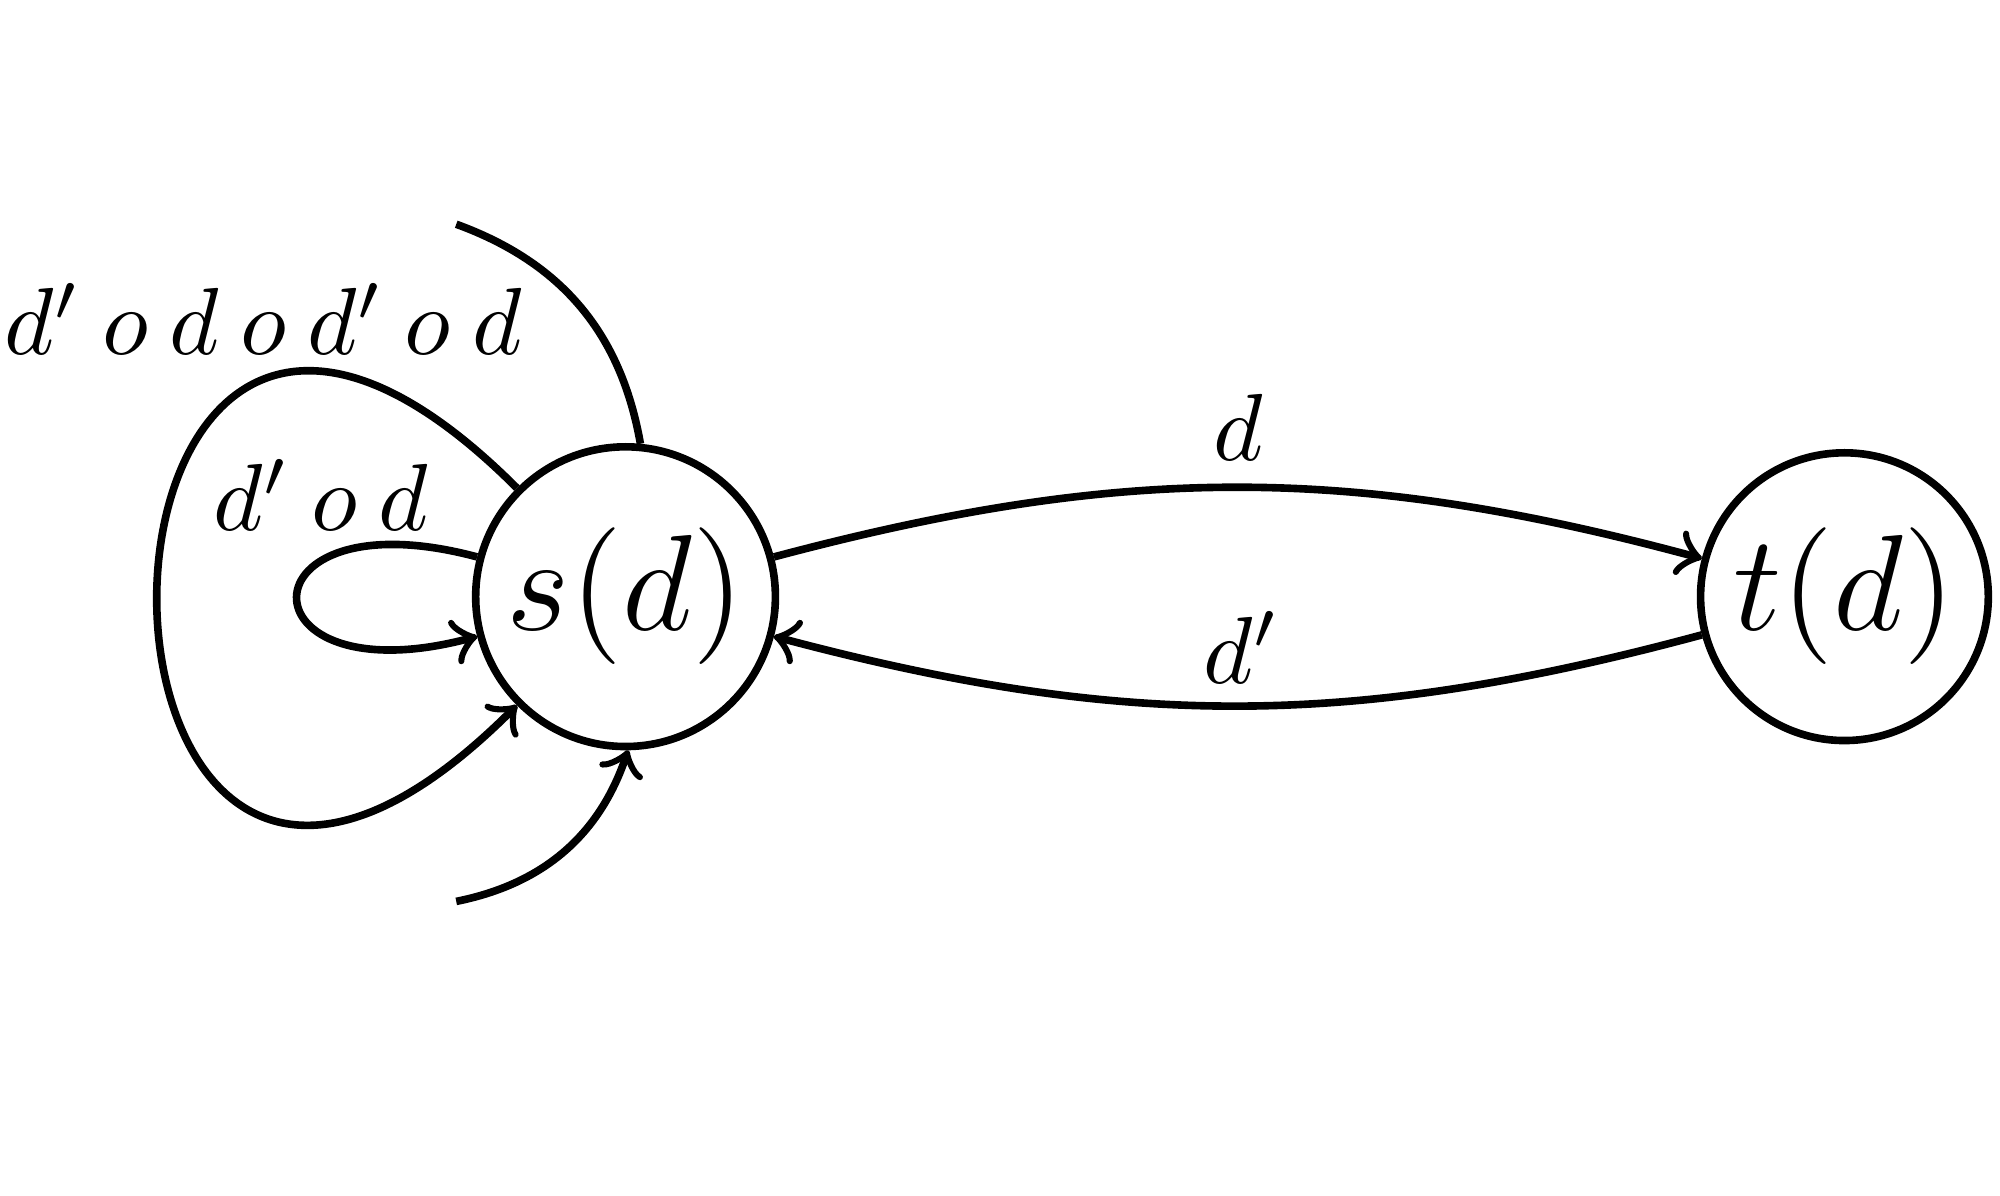
\includegraphics[width=1.0\linewidth]{2MathematicalFramework/Images/D_commonly_large.png}
		% \captionof{figure}{Test caption.}
		\caption{A world diagram showing sequences of the transformations $d$ and $d'$ that are of the form $(d' \circ d)^{n}$.}
	\end{center}
}, we do not show all the transformations in $D$ in our world diagrams unless explicitly stated.
When drawing the world diagram for a world $\mathscr{W}$, we default to drawing the vertices and arrows of the atomic multidigraph $\hat{\mathscr{W}}$ and the trivial transformations in $D_{\varepsilon}$.

\newthought{Let's look at} some world diagrams show casing some of the properties we've already seen.
\draftnote{blue}{Consider}{
Put these in the margin as we go, then say something about how these are the sort of diagrams we mean ?
}

\begin{figure}[H]
	\centering
	\begin{subfigure}[b]{0.45\linewidth}
		\centering
		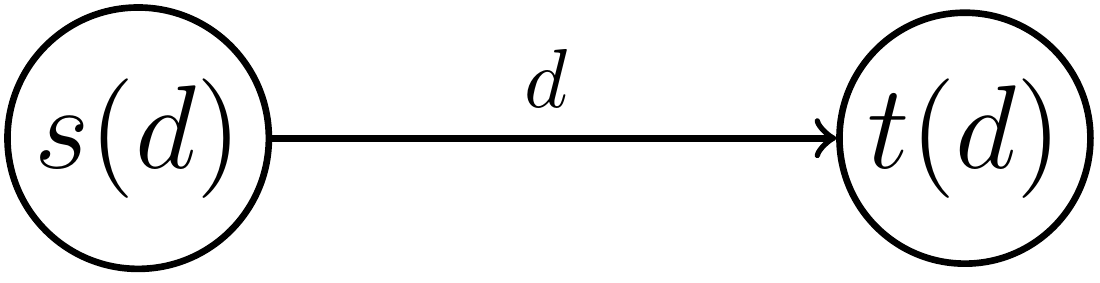
\includegraphics[width=\linewidth]{2MathematicalFramework/Images/transformation.png}
		\caption{A world diagram showing a transformation.}
		\label{fig:transformation}
	\end{subfigure}
	\hfill
	\begin{subfigure}[b]{0.45\linewidth}
		\centering
		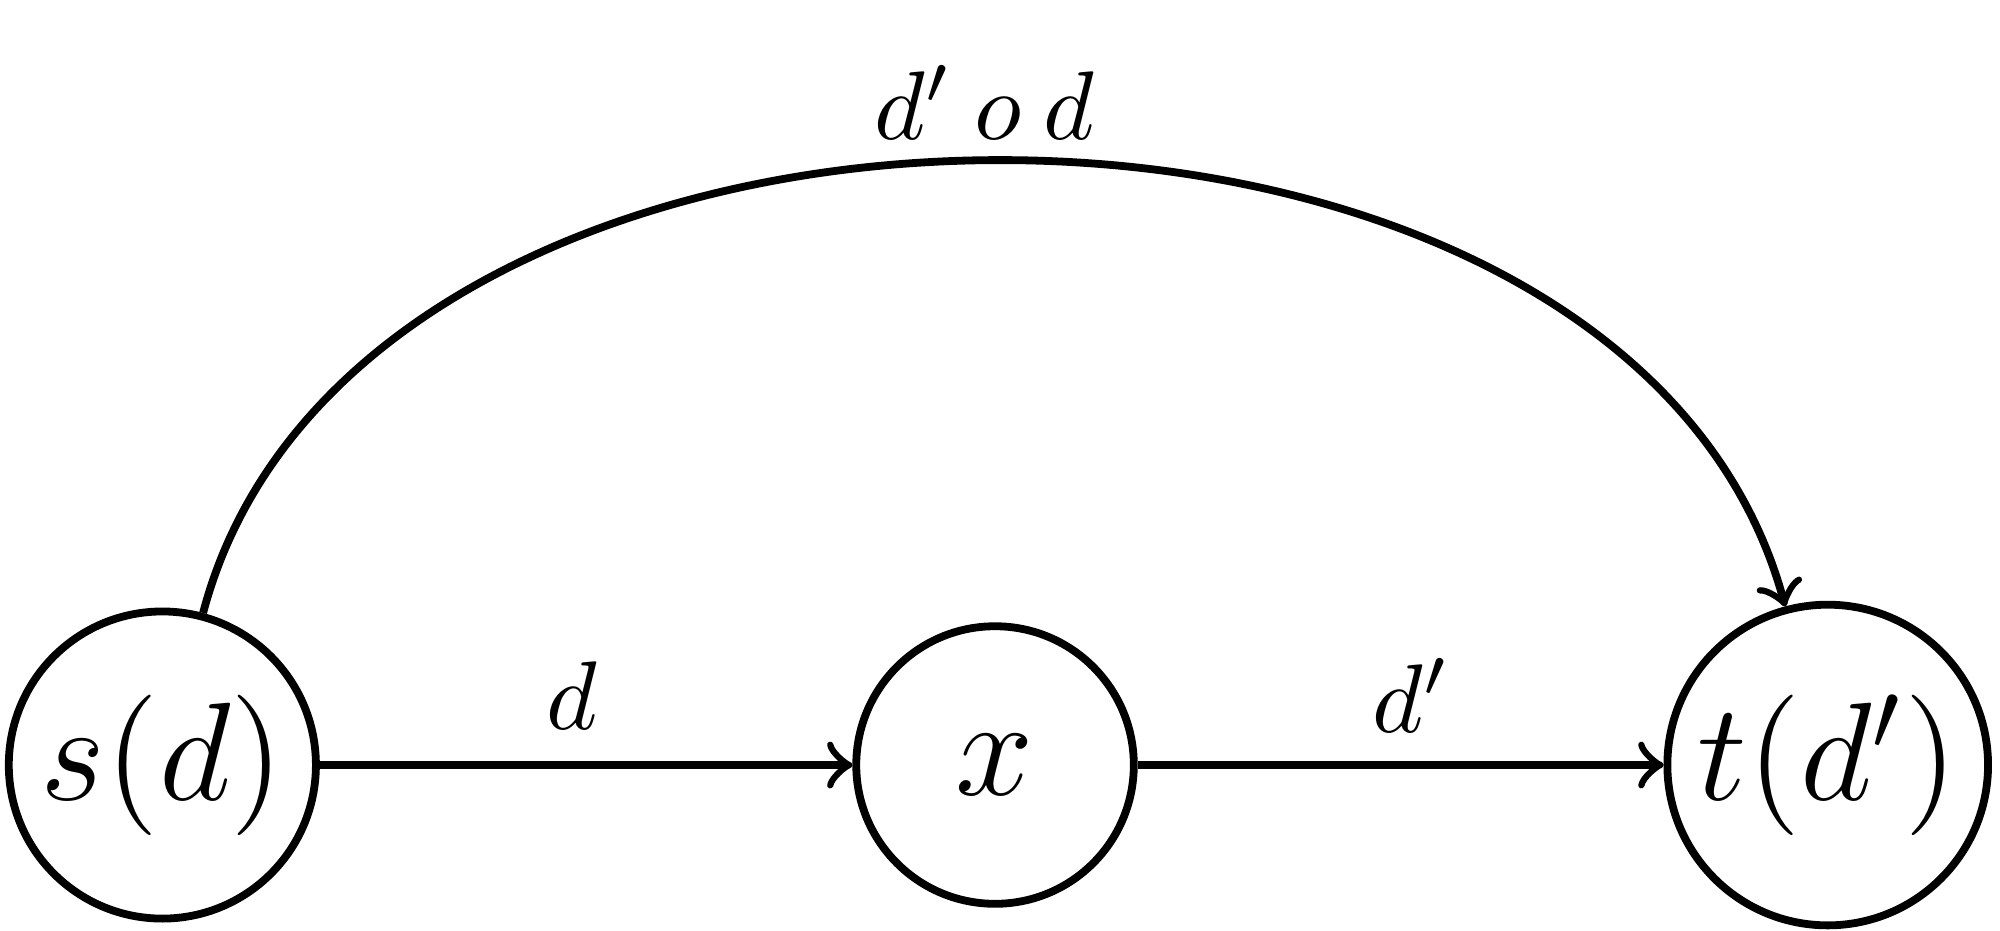
\includegraphics[width=\linewidth]{2MathematicalFramework/Images/transformation_composition.png}
		\caption{A world diagram showing the composition of two transformations $d$ followed by $d'$ to give a transformation $d' \circ d$.}
		\label{fig:transformation_composition}
	\end{subfigure}
	\vskip\baselineskip
	\begin{subfigure}[b]{0.45\linewidth}
		\centering
		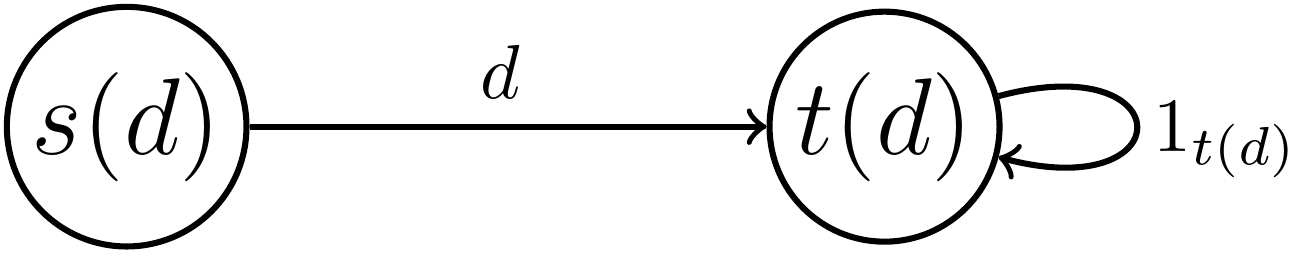
\includegraphics[width=\linewidth]{2MathematicalFramework/Images/left_trivial_transformation.png}
		\caption{A world diagram showing a transformation $d: s(d) \to t(d)$ and its left identity element, the trivial transformation $1_{t(d)}$. Composing these two transformations gives the transformation $d$.}
		\label{fig:left_trivial_transformation}
	\end{subfigure}
	\hfill
	\begin{subfigure}[b]{0.45\linewidth}
		\centering
		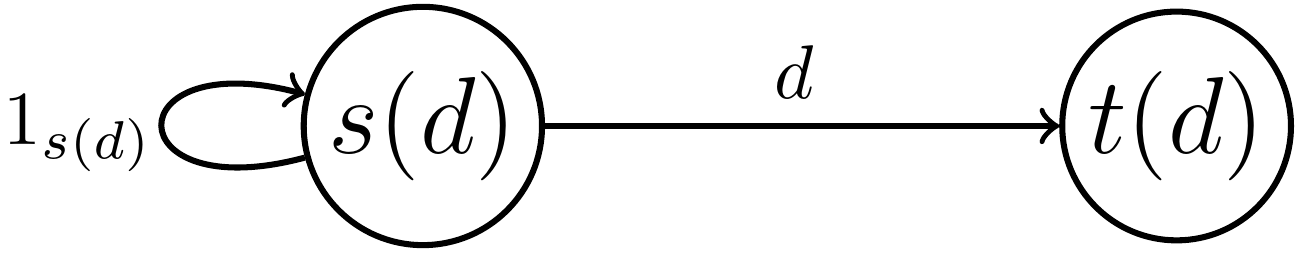
\includegraphics[width=\linewidth]{2MathematicalFramework/Images/right_trivial_transformation.png}
		\caption{A world diagram showing a transformation $d: s(d) \to t(d)$ and its right identity element, the trivial transformation $1_{s(d)}$. Composing these two transformations gives the transformation $d$.}
		\label{fig:right_trivial_transformation}
	\end{subfigure}
	\vskip\baselineskip
	\begin{subfigure}[b]{0.45\linewidth}
		\centering
		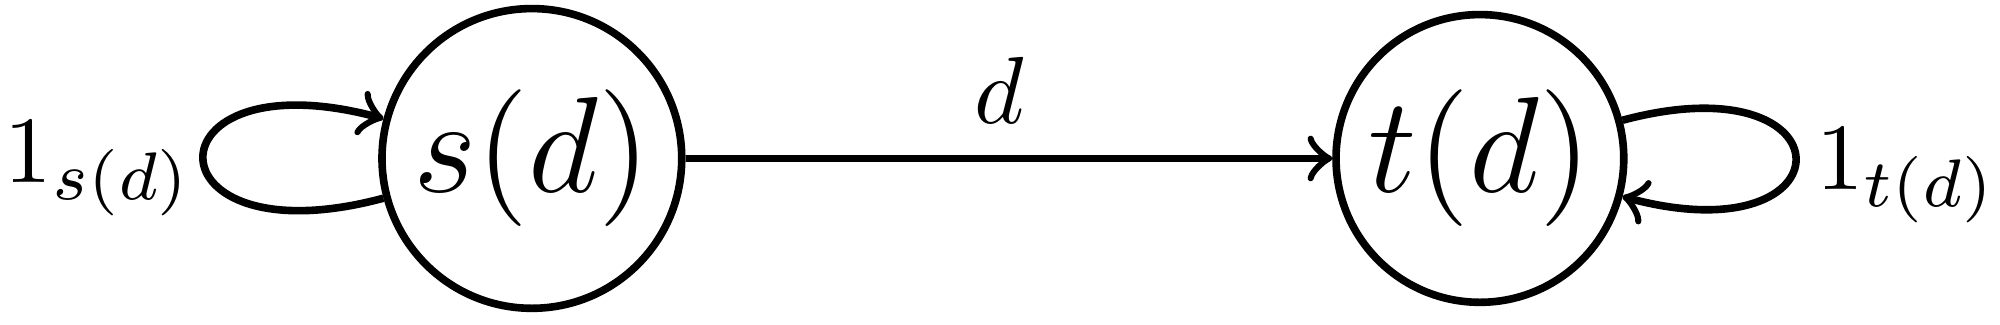
\includegraphics[width=\linewidth]{2MathematicalFramework/Images/trivial_transformations_example_all_transformations.png}
		\caption{A world diagram showing a transformation $d: s(d) \to t(d)$, its left identity $1_{t(d)}$, and its right identity $1_{s(d)}$.}
		\label{fig:trivial_transformations_example_all_transformations}
	\end{subfigure}
	\caption{Examples of world diagrams displaying some of the concepts we have already come across.}
\end{figure}

It's important to note that, in a world diagram, the positioning (relative or absolute) of the world states and the shapes and lengths of the arrows do not matter:
\begin{figure}[H]
    \centering
    \begin{tikzpicture}
        \node (left) {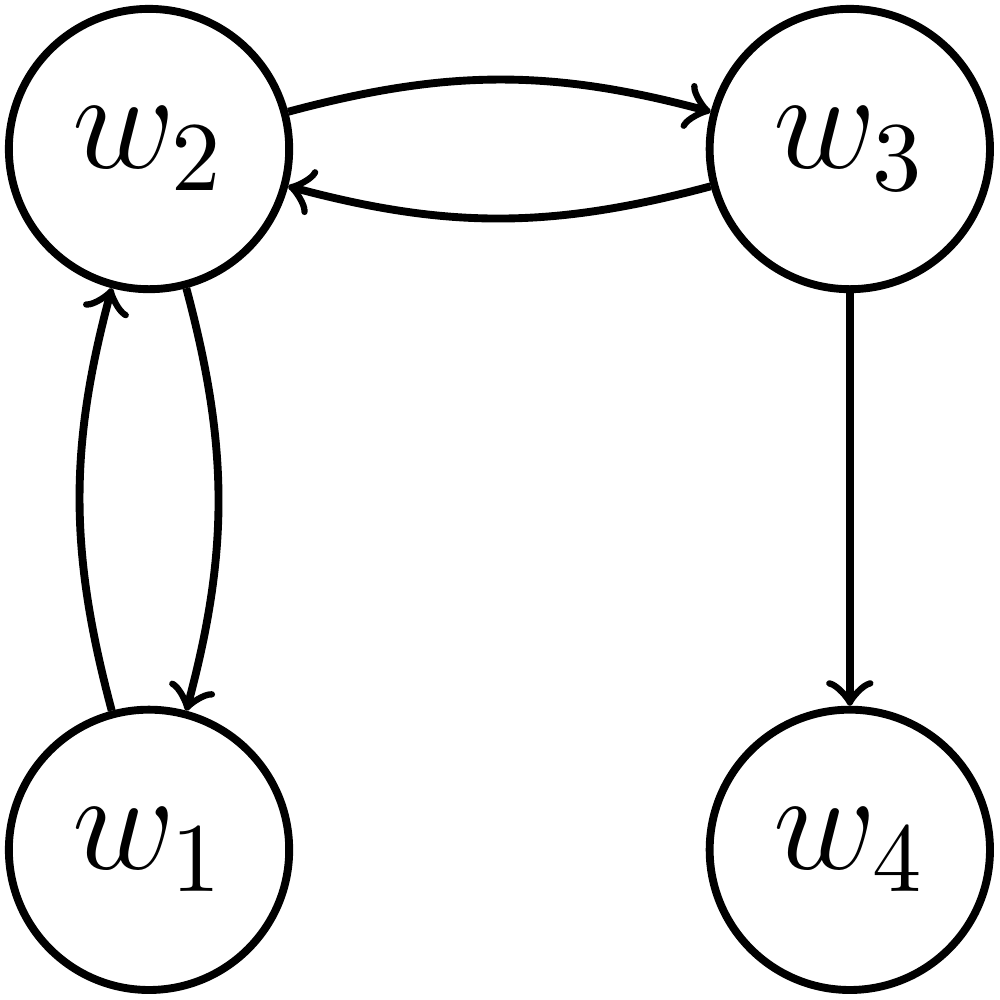
\includegraphics[width=0.3\textwidth]{2MathematicalFramework/Images/isomorphic_world_diagrams_1.png}};
        \node (sim) [right=1cm of left] {\Huge$\cong$};
        \node (right) [right=1cm of sim] {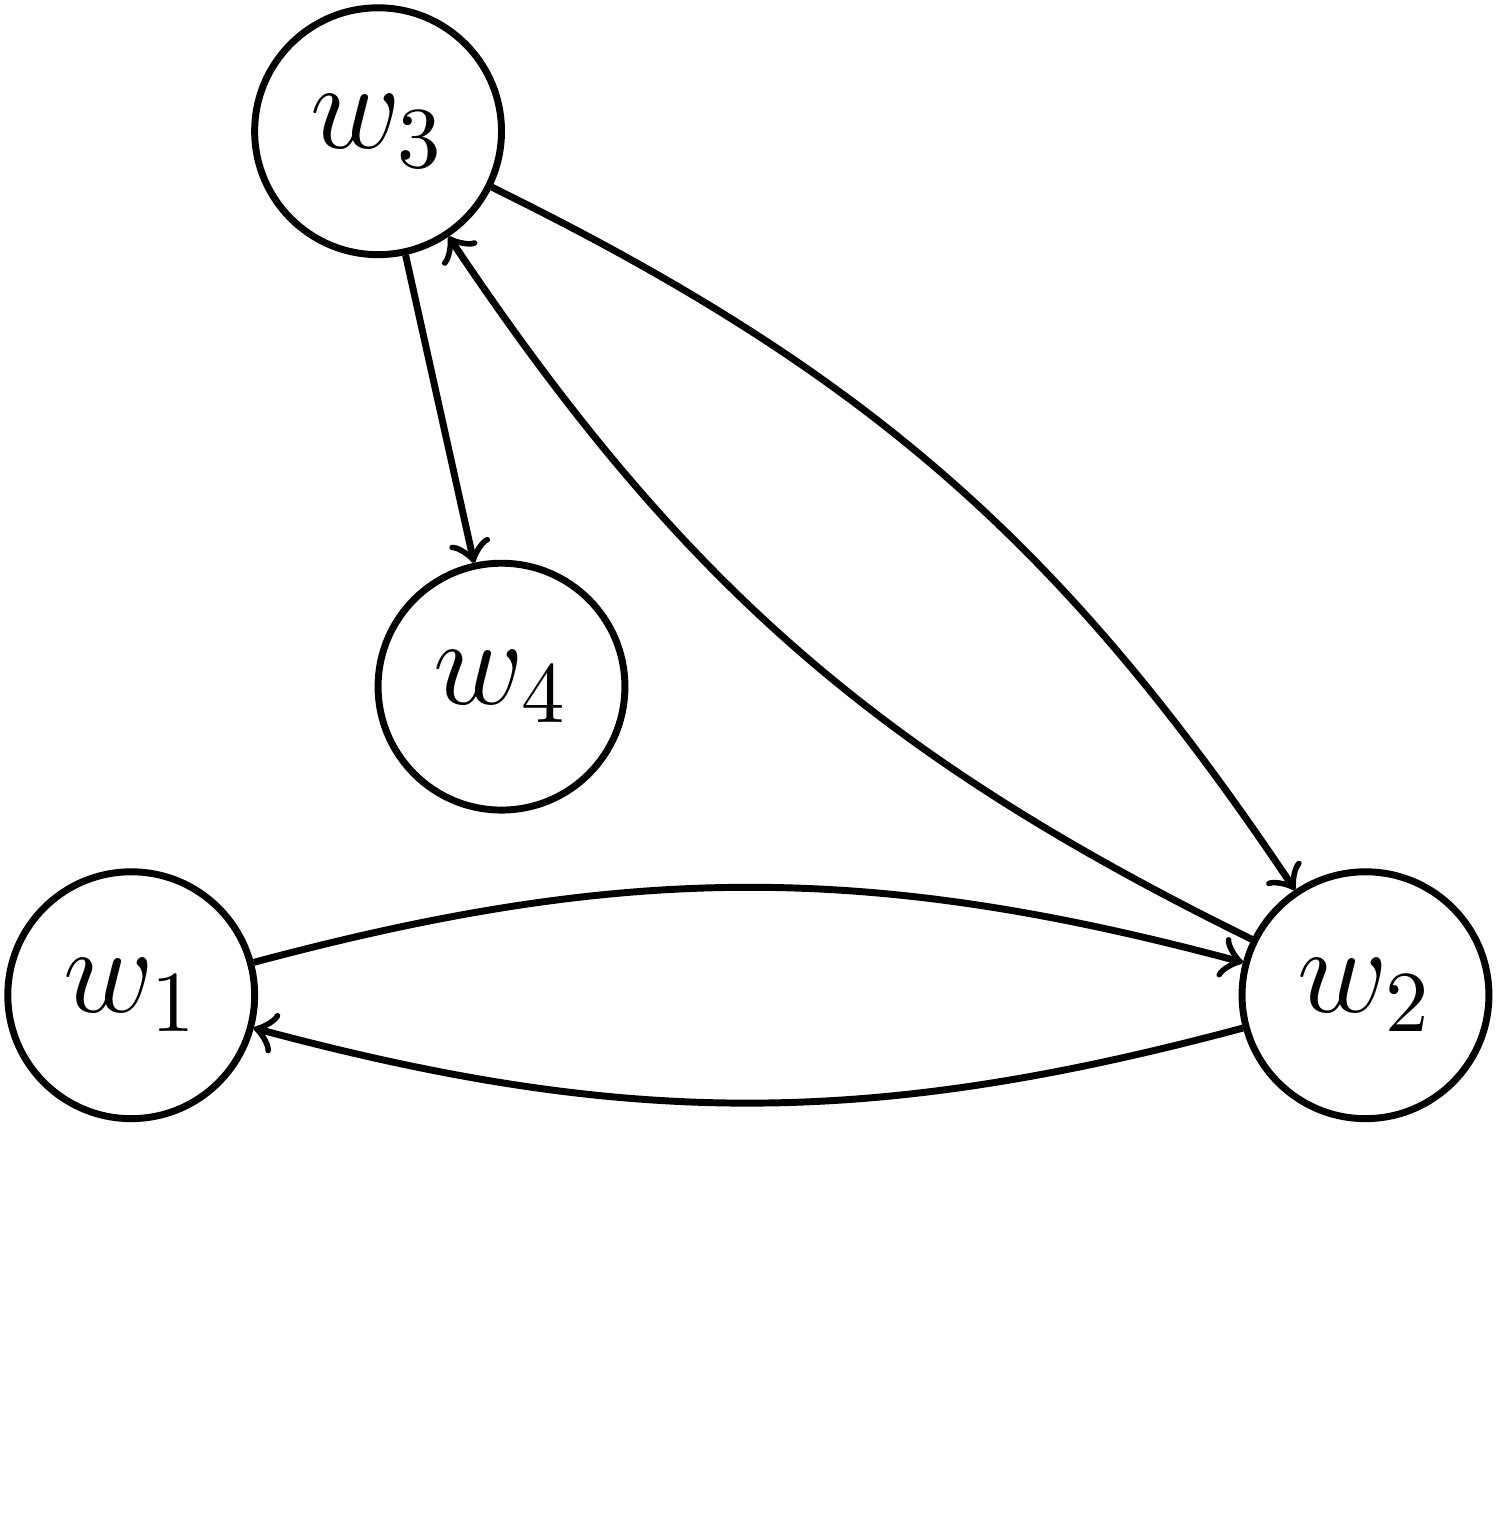
\includegraphics[width=0.4\textwidth]{2MathematicalFramework/Images/isomorphic_world_diagrams_2.png}};
    \end{tikzpicture}
    \caption{
    The properties of these world diagrams are identical (the world diagrams are isomorphic).
    }
    \label{fig:isomorphic_world_diagrams}
\end{figure}

%%%%%%%%%%%%%%%%%%%%%%%%%%%%%%%%%%%%%%%%%%%%%%%%%
\subsection{Subworlds}

\newthought{We are building} towards describing the structure of transformations in an agent's representation; later we will only be interested in the perspective of the agent and so will only care about the world states and transformations that the agent can interact with.
Reachable and unreachable subworlds give us the language to describe and then disregard parts of worlds that agents will never explore and therefore are not relevant to the agent's representation.
For example, if an agent is in a maze and a section of the maze is inaccessible from the position that the agent is in, then that section of the maze would be disconnected from the section of the maze that the agent is in; if we want to study how the agent’s representation evolves as it learns, it makes sense to disregard world states where the agent is in the inaccessible part of the maze since those world states can never be reached and so those world states will not affect the agent's representation.
\footnote{
	But what about worlds that are unreachable from the current world state, but the agent has already visited?
	If we assume the representation evolution process is Markov, then all the necessary information will contained in the current representation space of the agent and so past world states which are now unreachable are irrelevant.
	Therefore, for a Markov representation evolution process, we only need to consider the world states in subworlds that are reachable from the current world state.

	If the representation evolution process is not Markov, we can transform the representation evolution process into a Markov process by augmenting the state space of the process to include any relevant historical information.
}


\newthought{When constructing a} subworld we want to preserve the composition $\circ$, so that a subworld is a world; this means we have to be careful which transformations we remove to form a valid subworld.
A world $\mathscr{W}' = (W', D', s', t')$ is a \emph{subworld} of a world $\mathscr{W} = (W, D, s, t)$ if
\begin{enumerate}
    \item $W' \subseteq W$;
    \item $D' \subseteq D$ such that:
    \begin{enumerate}
        \item For all $d \in D'$, $s(d) \in W'$ and $t(d) \in W'$;
        \item For all $d, d' \in D'$ with $d: s(d) \to t(d)$ and $d': t(d) \to t(d')$, $d \circ d' \in D'$;
        \item For all $w' \in W'$, $1_{w'} \in D'$;
    \end{enumerate}
    \item $s'$ is the restriction of $s$ to $D' \to W'$;
    \item $t'$ is the restriction of $t$ to $D' \to W'$\footnote{
    We usually use $s$, $t$ instead of explicitly defining the maps $s'$ and $t'$ because $s$ and $t$ act on all the elements of $D$ and $D'$ is a subset of $D$.
    }.
\end{enumerate}

\begin{notation}
    If $\mathscr{W}'$ is a subworld of $\mathscr{W}$ then we can write $\mathscr{W}' \subseteq \mathscr{W}$.
\end{notation}

If $\mathscr{W}' \subseteq \mathscr{W}$, then the atomic multidigraph of $\mathscr{W}'$ is not necessarily a sub-multidigraph of the atomic multidigraph of $\mathscr{W}$; in other words, $\mathscr{W}' \subseteq \mathscr{W}$ does not necessarily mean $\hat{D}' \subseteq \hat{D}$. For example, if $\hat{d}_{1}, \hat{d}_{2} \in \hat{D}$ and $\operatorname{Seq}(d_{3}) = (\hat{d}_{2}, \hat{d}_{1})$, it is possible to have a subworld where $\hat{d}_{1}, \hat{d}_{2} \centernot\in D'$ (and so $\hat{d}_{1}, \hat{d}_{2} \centernot\in \hat{D}'$) but have $d_{3} \in D$.
In this case, $d_{3}$ would be an atomic transformation in $\mathscr{W}'$ (i.e., $d_{3} \in \hat{D}'$).\footnote{
\begin{figure}[H]
    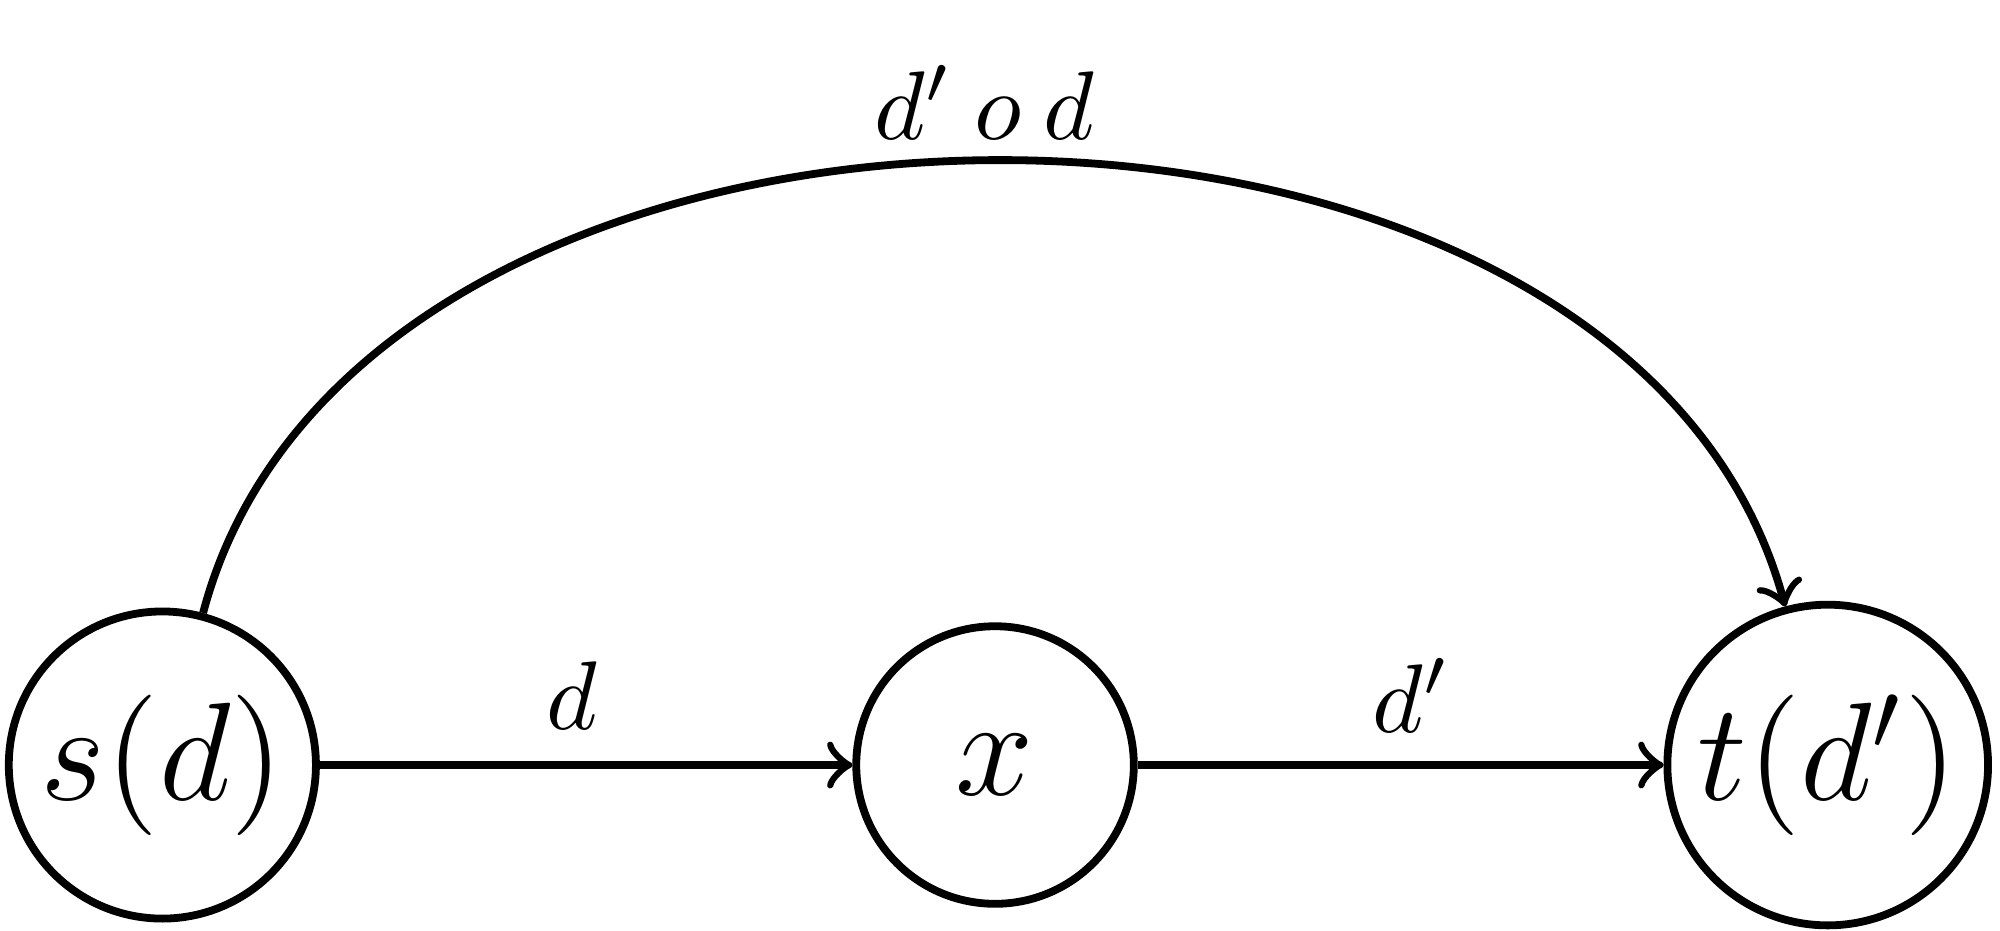
\includegraphics[width=0.5\linewidth]{2MathematicalFramework/Images/transformation_composition.png}
    \caption{
    If $d_{3} = d_{2} \circ d_{1}$ and $d_{1}, d_{2} \in \hat{D}$, then when constructing a subworld we can remove $d_{1}$ and $d_{2}$ and keep $d_{3}$ (in which case $d_{3}$ would be an atomic transinformation in the subworld), but we cannot remove $d_{3}$ without removing $d_{1}$ and $d_{2}$.
    }
\end{figure}
}
More generally, suppose $\mathscr{W}' \subseteq \mathscr{W}$; for $d \in D$ and $\operatorname{Seq}(d) = (\hat{d}_{n}, \hat{d}_{n-1}, \dots, \hat{d}_{1})$, if $\hat{d}_{n}, \hat{d}_{n-1}, \dots, \hat{d}_{1} \centernot\in \hat{D}'$, then either $d \in \hat{D}'$ or $d \centernot\in D$.
\draftnote{purple}{PS: Consider}{Is this a proposition we need to prove ?}
\footnote{
This property of subworlds allows us to construct discrete worlds out of continuous worlds by, for example, removing atomic transformations that cannot be perceived by an agent.
}
When constructing subworlds from a world, if removing atomic transformations causes another transformation to become an atomic transformation in the subworld, the number of atomic transformations in the subworld will decrease.
Therefore, we have
\begin{equation}
    \mathscr{W}' \subseteq \mathscr{W} \implies |\hat{D}'| \leq |\hat{D}|
\end{equation}
\draftnote{purple}{PS: Consider}{Is this a proposition that we need to prove ?}


%%%%%%%%%%%%%%%%%%%%%%%%%%%%%%%%%%%%%%%%%%%%%%%%%
\paragraph{Reachable and unreachable subworlds.}
\newthought{Consider a world} $\mathscr{W}^{\aleph}$ containing two subworlds $\mathscr{W}$ and $\mathscr{W}'$.
The subworld $\mathscr{W}'$ is \emph{reachable} from the subworld $\mathscr{W}$ if there exists a transformation $d \in D^{\aleph}$ with $d: w \to w'$ where $w \in W$ and $w' \in W'$.\footnote{
\begin{figure}[H]
	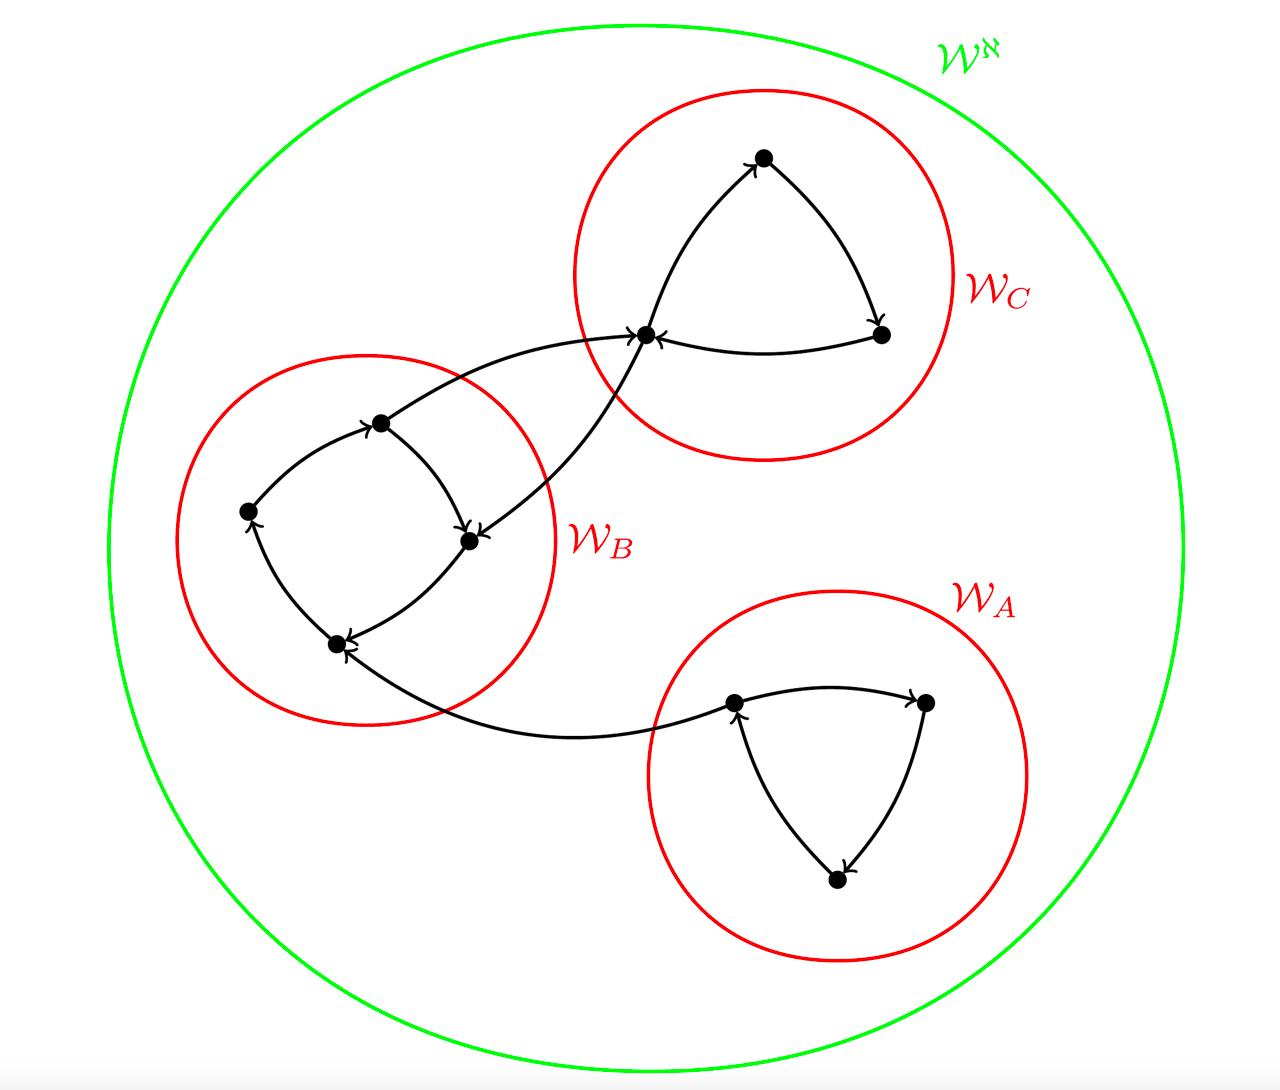
\includegraphics[width=0.5\linewidth]{2MathematicalFramework/Images/reachable_worlds.jpeg}
	\caption{
		$\mathscr{W}_{C}$ is reachable from $\mathscr{W}_{A}$ and $\mathscr{W}_{B}$, but $\mathscr{W}_{A}$ is not reachable from $\mathscr{W}_{B}$ or $\mathscr{W}_{C}$.
	}
	\label{fig:reachable_worlds}
\end{figure}
}
If a subworld is not reachable, we say it is \emph{unreachable}.

Formally, for a world $\mathscr{W} = (W, \hat{D}, s, t)$, the set of world states that are reachable from a world state $w$ is given by
\begin{equation}
	W^{\to}(w) := \{ w' \in W \mid \text{ there exists } d \in D \text{ with } d: w \to w' \}.
\end{equation}
The set of atomic transformations that are reachable from $w$ is given by\footnote{
	This is the largest subset of atomic transformations that stay within the set of reachable states.
}
\begin{equation}
	\hat{D}^{\to}(w) := \{ \hat{d} \in \hat{D} \mid s(\hat{d}) \in W^{\to}(w) \; \text{and} \; t(\hat{d}) \in W^{\to}(w) \}
\end{equation}

The atomic multigraph of the \emph{reachable subworld} of a world $\mathscr{W}$ from the state $w$ is given by
\begin{equation}
	\hat{\mathscr{W}}^{\to}(w) := (W^{\to}(w), \hat{D}^{\to}(w), s \big|_{D^{\to}(w)}, t \big|_{D^{\to}(w)})
\end{equation}
The reachable subworld $\mathscr{W}^{\to}(w)$ of $\mathscr{W}$ from the state $w$ is then constructed using $\hat{\mathscr{W}}^{\to}(w)$ in the usual way.

\begin{notation}
	We denote the current world state by $w^{*}$.
\end{notation}

The subworld that is reachable from the current world state $w^{*}$ is called the \emph{natural reachable subworld}, which we denote by $\mathscr{W}^{\to}(w^{*})$.

%%%%%%%%%%%%%%%%%%%%%%%%%%%%%%%%%%%%%%%%%%%%%%%%%%%%%%%%%

%%%%%%%%%%%%%%%%%%%%%%%%%%%%%%%%%%%%%%%%%%%%%%%%%%%%%%%%%
\section{Introducing an agent}

\newthought{We want to} study the structure of the representations of an agent that can interact with a world.
But before we can study the structure of an agent's representations, we need to define what an agent and its representations are in our framework.

%%%%%%%%%%%%%%%%%%%%%%%%%%%%%%%%%%%%%%%%%%%%%%%%%%%%%%%%%
\subsection{What is an agent ?}

\newthought{An \emph{agent} is} an autonomous entity\footnote{This could be a natural or artificial entity.} that can observe and interact with its environment\footnote{Our agent does not need to be embodied in the world - more on this later !}; the agents that we care about can also learn about their environments.

%%%%%%%%%%%%%%%%%%%%%%%%%%%%%%%%%%%%%%%%%%%%%%%%%%%%%%%%%
\subsection{Representations of an agent}

\newthought{An agent's \emph{representation states}} are the agent's internal representations of world states, through which the agent maintains its understanding of its world.
An agent's \emph{representation model} is the agent's internal model of the world, which includes how the agent encodes and organises information about its environment (e.g., as vectors, symbols, or other data structures) as representation states as well as the dynamics of how those representation states change due to actions that affect the world\footnote{
	The agent's representation model does not directly encode the dynamics of the world states, it encodes the dynamics of the representation states; a `good' representation will provide a good approximation to the dynamics of the world states.
}.
The agent's representation model not only captures the current state of the world but also allows the agent to conceptualise future world states by predicting the wporld state that will our from the current world state when an action is applied; this allows the agent to plan future actions, and so form a comprehensive framework for decision-making and interaction.

\newthought{Agents use \emph{sensors}} to capture data from their world, enabling the agent to perceive the world; these sensors include real-world sensors (e.g., cameras on a robot, the human eye) and virtual inputs (e.g., data streams, user commands).
Sensors provide the agent with \emph{observation states}\footnote{In some literature, observation states are called \emph{sensory states} such as in \cite{Ramstead2020}.}, which are the agent's internal representations of the information the sensors collect (e.g., data streams from the camera)\footnote{
	Importantly, obervation states are not the sensors themselves.
}.
An agent's \emph{perceptual model} is how the agent encodes and organises information from its sensors (e.g., vectors, symbols, or other data structures) as well as how it conceptualises the structure of the landscape of possible observation states.

\newthought{Agents use \emph{effectors}} to interact with and alter worlds.
Effectors enable agents to carry out actions in the world; effectors can be real-world effectors (e.g., motors and actuators on a robot) or virtual outputs (e.g., API calls or applying a transformation to a dataset the agent is manipulating).
Effectors receive \emph{effector signals}\footnote{
Effector signals are commonly called \emph{control signals} in the field of robotics.
}, which are the concrete instructions sent by the agent to perform actions (e.g., a voltage spike sent to a motor or a command sent to a software interface).
An agent also has an \emph{action model}, which is how the agent encodes and organises information about its actions (e.g., control signals, symbolic commands) as well as how it conceptualises how its actions will affect the world state.
An agent's action model is intrinsically linked to its representation model since the action model describes the movement between representation states of the representation model due to actions\footnote{
These actions do not have to be only the actions of the agent itself, they can be a grouping of world state transformations that the agent understands to be from a particular cause (see \draftnote{blue}{section ???}{}).
}.

%%%%%%%%%%%%%%%%%%%%%%%%%%%%%%%%%%%%%%%%%%%%%%%%%%%%%%%%%
\subsection{Agents as Markov blankets}

\newthought{In our framework}, we consider agents to be systems with internal states that interact with the world such that a boundary is maintained between their internal states and the world.
Agent's in our framework have four types of state:
\begin{enumerate}
	\item \emph{Observation states} represent the agent's inputs from the environment (e.g., vision, sound, touch etc...).
	\item \emph{Effector states} represent how the agent influences the world state (i.e., the agent's external environment).
	\item \emph{(External) world states} consist of the states of the agent's external environment, which are the world states we introduced in \cref{sec:A mathematical treatment of worlds and their transformations}.
	\item \emph{Agent's (internal) representation states} contain our agent's representations of the environment, memory model, knowledge models, goals, decision making processes etc...
	      These internal states can only interact with the external world states via observation states and effector states.
\end{enumerate}

Using these four types of states we can view our agents as Markov blankets (see \cref{fig:markov_blanket})]
\draftnote{blue}{Consider}{
	Is the agent a Markov blanket or is it surrounded by a Markov blanket ???
}
.

\begin{figure}[H]
	\centering
	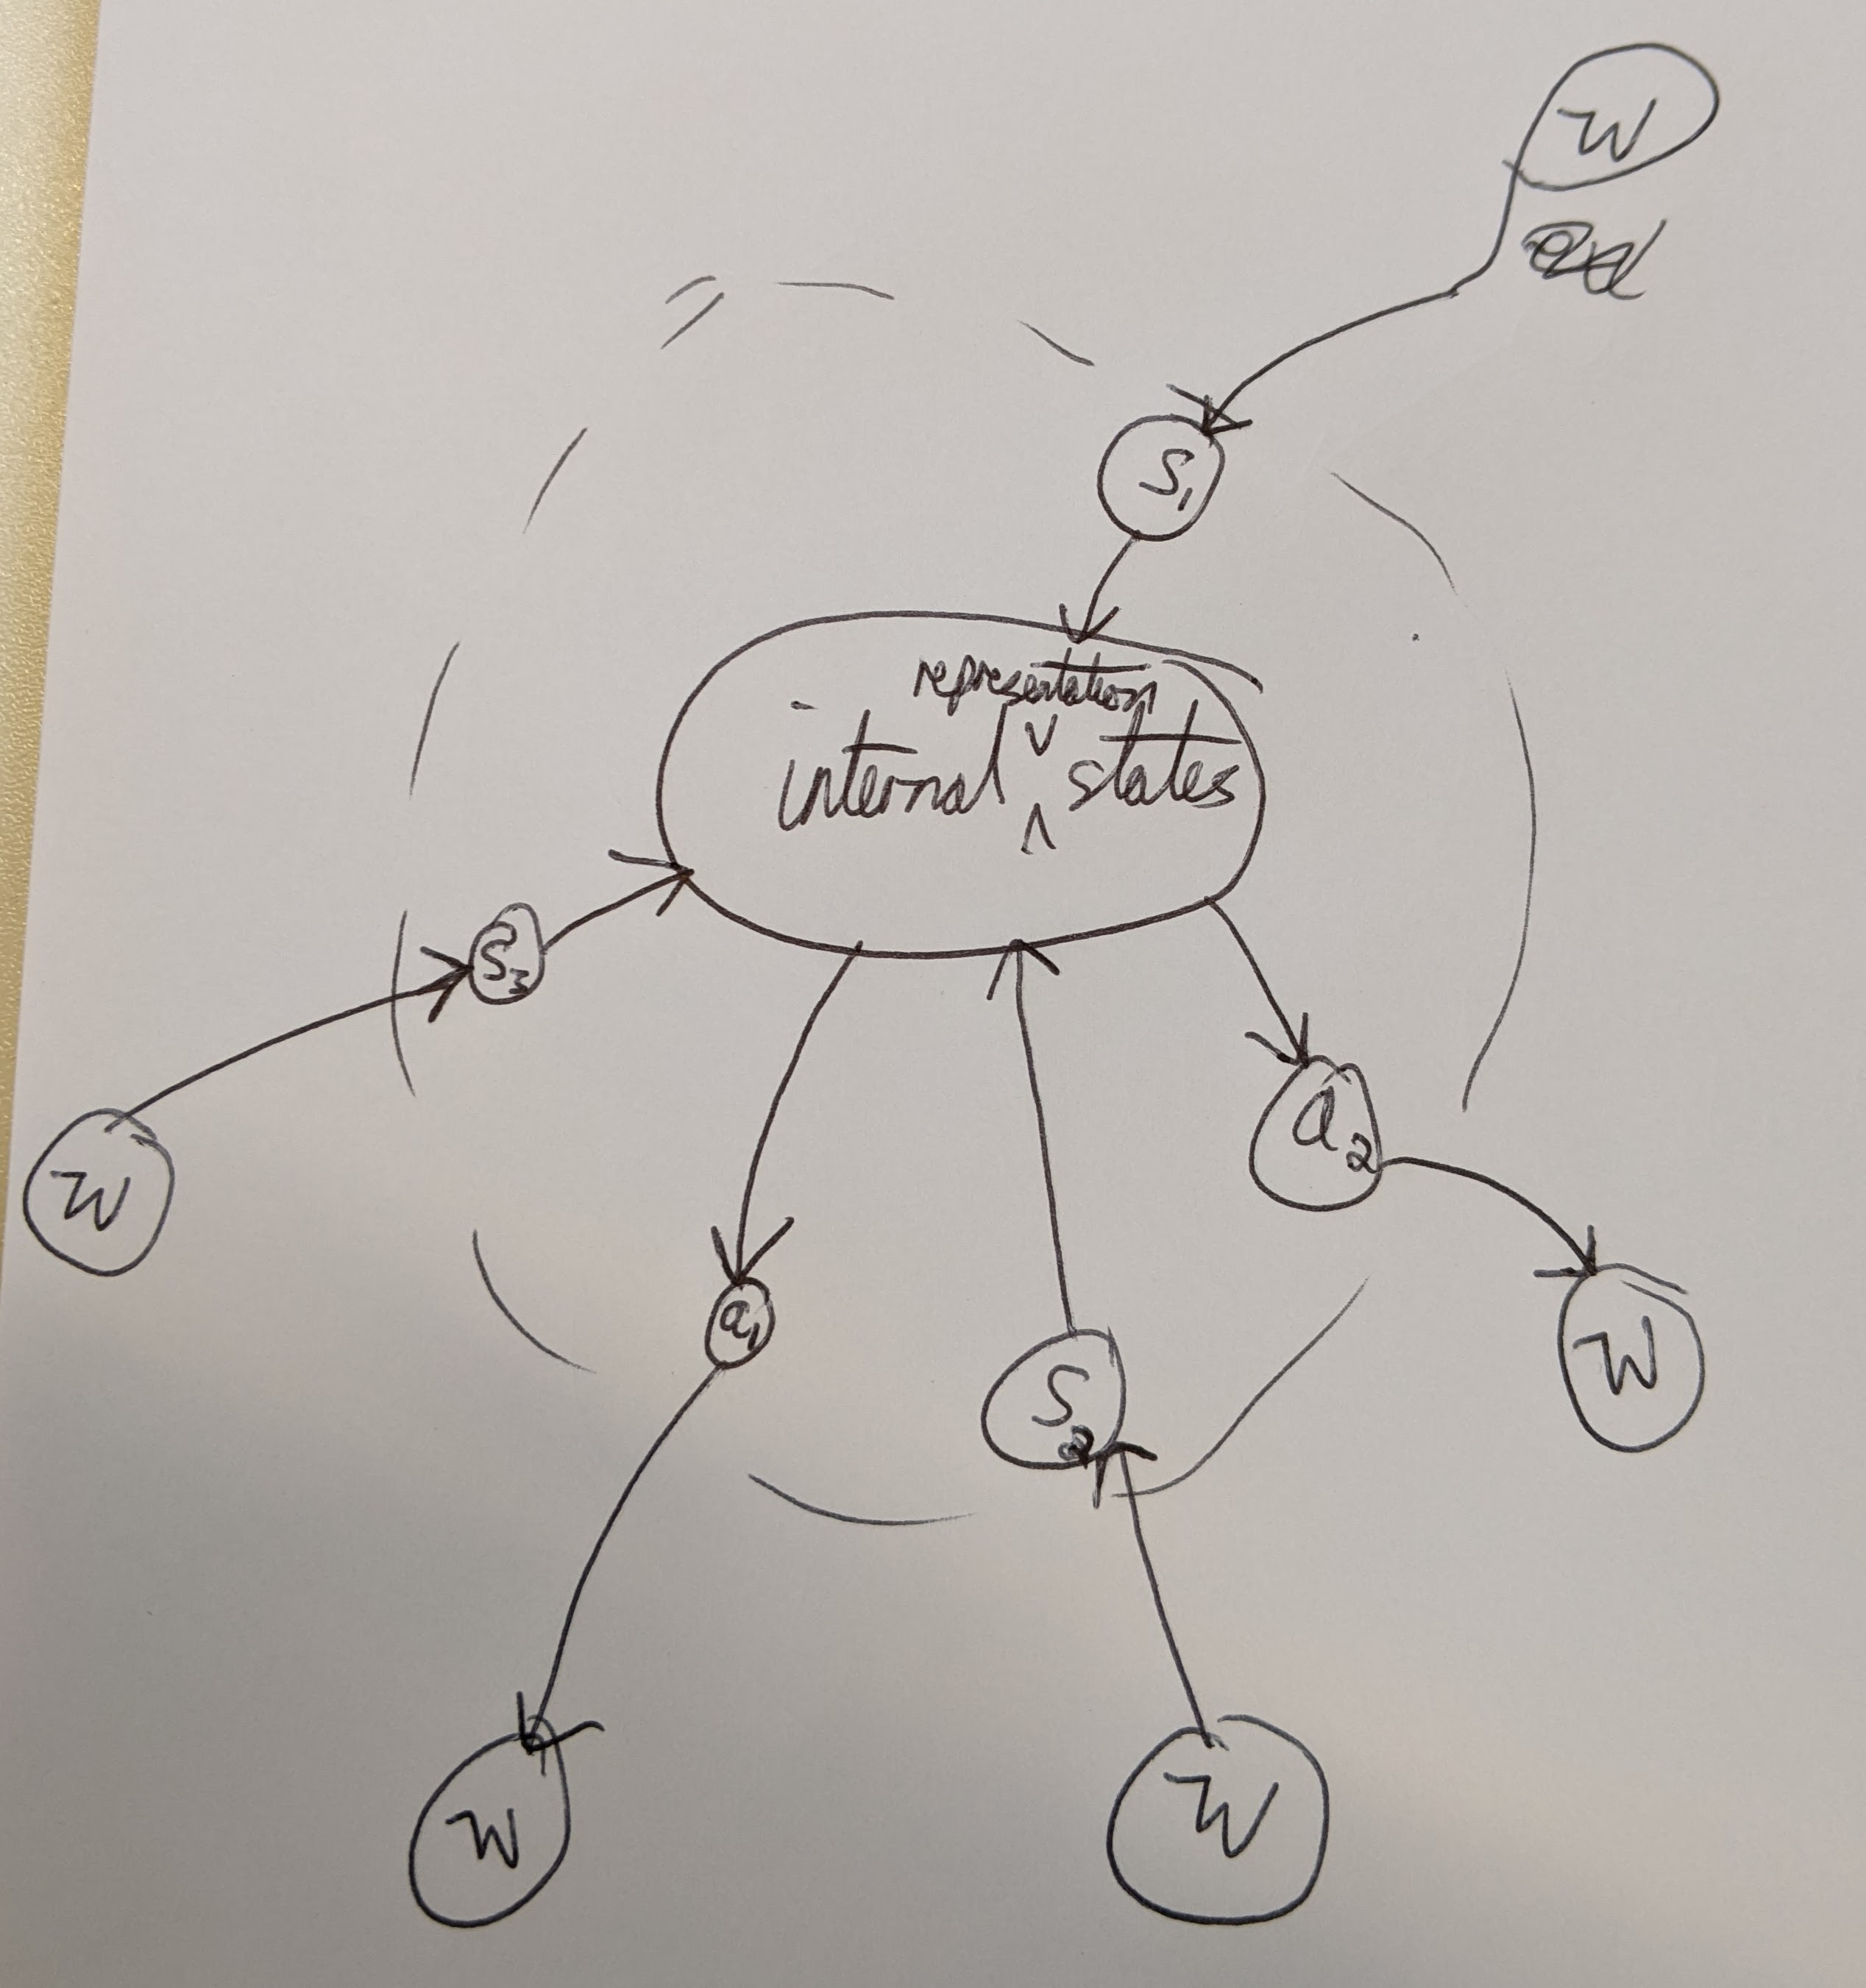
\includegraphics[width=0.5\linewidth]{2MathematicalFramework/Images/markov_blanket.jpg}
	\caption{
		Complete caption.
		Arrows show the flow of information.
	}
	\label{fig:markov_blanket}
\end{figure}

The Markov blanket consists of the states that mediate interactions between our agent and its environment (the world) \cite{Ramstead2020}.

\newthought{For an agent} in our framework, the observation and effector states form the Markov blanket with the world states being outside the blanket and the the internal state being inside the blanket.
This Markov blanket acts as a boundary that separates the agent's internal representation states from the external world states.
The agent can not directly access the world states, but it can infer the structure of these world states by processing sensory inputs through its observation states and performing actions through its effector states; information about the world states crosses the Markov blanket through the agent's sensory states and the agent's affect on the world crosses the Markov blanket through the agent's effector states.

\begin{postulate}
	An agent consists of internal representation states separated from external world states by a Markov blanket consisting of observation states, through which the agent receives information about the world states, and effectors, through which the agent can change the world state.
\end{postulate}

Technically, given the observation and effector states (i.e., the blanket), the internal representation states of the agent are \emph{conditionally independent} of the external world states; conditionally independent of the external world states means that the behaviour of the agent's internal representation depends only on the states of the agent's Markov blanket (i.e., the agent's observation and effector states) and not (directly) on the world states external to the agent because all the relevant information about the external world states are filtered through the observation states and the agent only affects the world through its effector states.

\newthought{By framing agents} as a Markov blankets, we aim to clearly show that agents learn about their world only through their observation states and their effectors.

A major implication of this approach for our framework is we consider the internal representation states of the agent to be separate from the world states introduced in \cref{sec:A mathematical treatment of worlds and their transformations}; this means that if we swap an agent embodied in a world with another agent that is identical except for having a different internal representation state (or a different representation model), then the world state would remain unchanged.

Another implication of our approach is that, since an agent's only gains knowledge about the structure of the world through its sensors and its actions, world states with differences that are not detectable by the agent are identical from the agent's perspective and so can be treated as such when we are constructing a mathematical description of the agent's interaction with the world (i.e, indistinguishable world states do not exist from the perspective of the agent, and so cannot appear in the agent's representation).


%%%%%%%%%%%%%%%%%%%%%%%%%%%%%%%%%%%%%%%%%%%%%%%%%%%%%%%%%
\subsection{Sensory perception}

\newthought{Our agent has} an unspecified number of sensors that allows it to make observations of the world.
Information about the agent's current world state is delivered to the agent's internal decision systems as an observation state; this is called the \emph{observation process}\footnote{
If the world state is modelled as a distribution then is process is also referred to as the agent \emph{sampling the world state}.
}.
For example, the human eye (the sensor) converts information about the light entering the eye into electrical signals in the optic nerve (the observation process); each particular collection of electrical signals (the observation state) is provided to the agent's internal decision mechanisms.

\newthought{Mathematically, we treat} the observation process as a mapping
\begin{equation}
\begin{aligned}
	& b: W \to O \\
	& \text{such that } b(w_{i}) = o_{i}
\end{aligned}
\end{equation}
where $w_{i} \in W$ is a world state and $o_{i} \in O$ the observation state produced by the observation process $b$.
The structure of $o_{i}$ depends on the agent's perceptual model; commonly, each observation $o_{i}$ is a vector of length $N$, where $N$ is the number of sensors the agent has.

\begin{figure}[H]
	\centering
	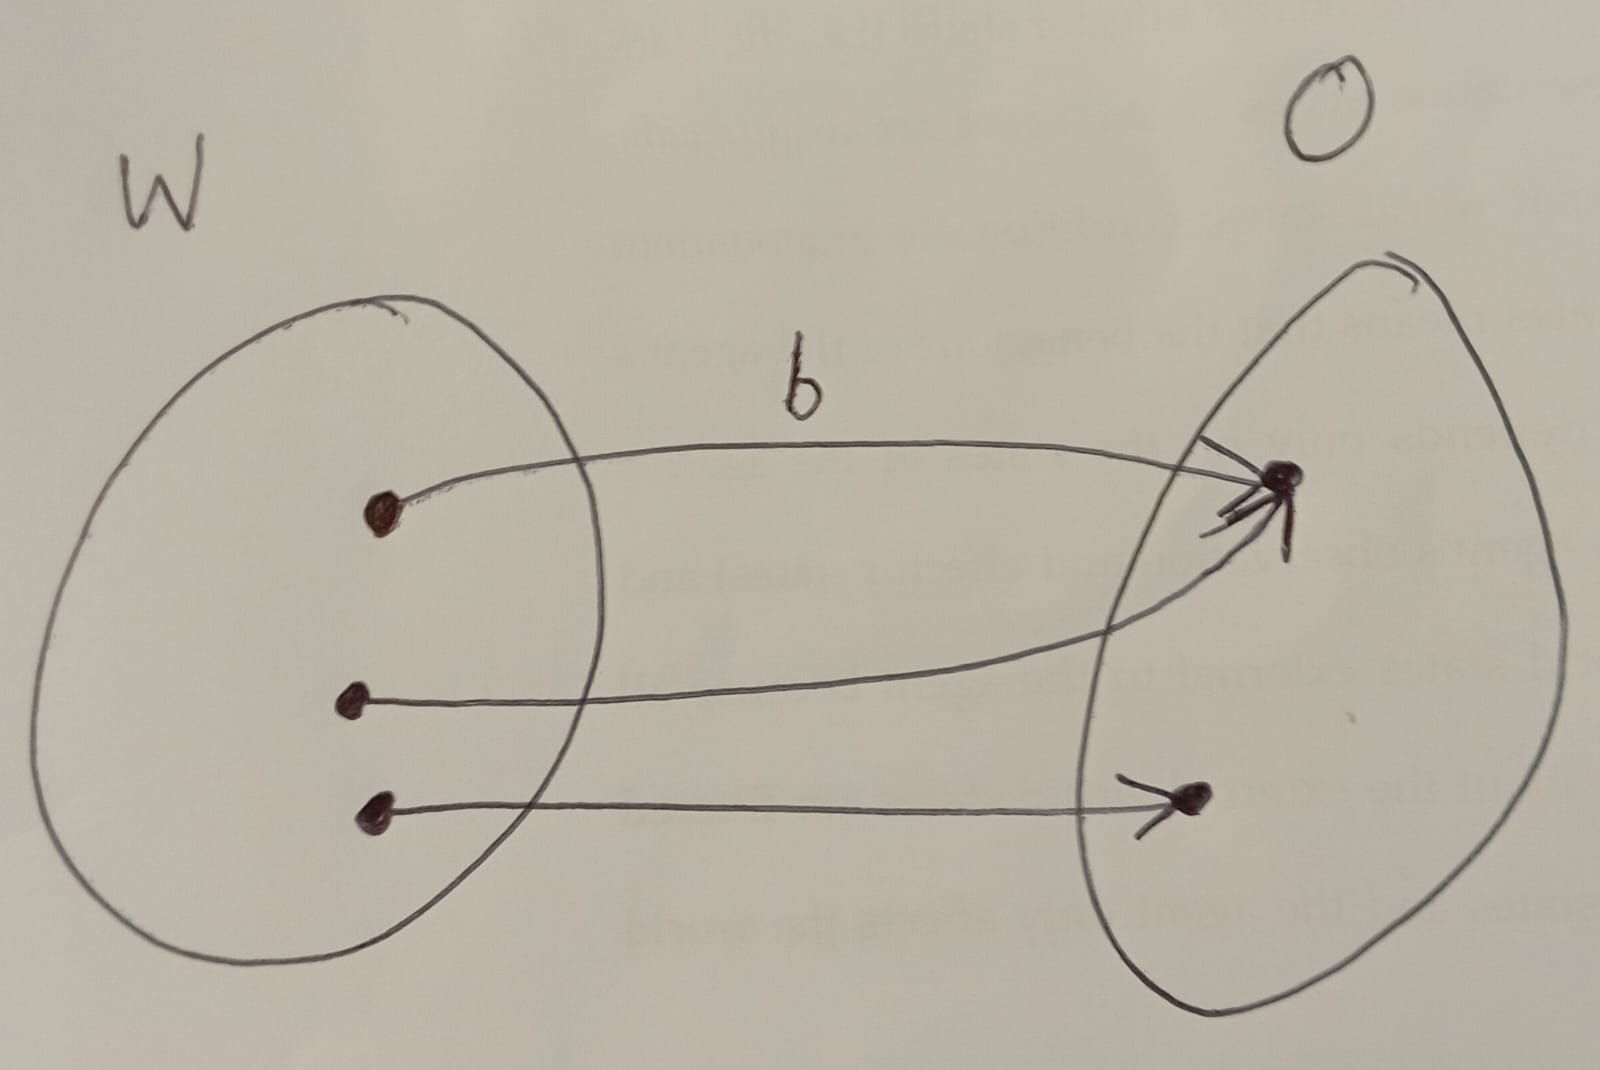
\includegraphics[width=0.5\linewidth]{2MathematicalFramework/Images/observation_process_W_to_O.jpeg}
	\caption{
		An example of how an observation process $b: W \to O$ sends each worlds state in $W$ to an observation state in $O$.
		Note how it is possible for two distinct world states to produce the same observation state.
	}
	\label{fig:observation_process_W_to_O}
\end{figure}


%%%%%%%%%%%%%%%%%%%%%%%%%%%%%%%%%%%%%%%%%%%%%%%%%%%%%%%%%
\paragraph{Ideal sensors.}

\newthought{In real-world situations}, it is common for information about the world state to be lost, modified or not picked up during the observation process (e.g., the human eye only picks up certain wavelengths of light or a camera could capture an image in a colour spectrum then output greyscale) or for distinct world states to produce the same observation state (e.g., worlds where objects can be hidden).

We say that an agent has \emph{ideal sensors}, if
\begin{enumerate}
	\item information is not lost or modified during the observation process;
	\item there is no noise in the obervation process; and
	\item for every distinct world state in $W$ the observation process produces a distinct observation states in $O$:
	\begin{equation}
		b(w) \neq b(w') \quad \text{for all $w,w' \in W$}.
	\end{equation}
\end{enumerate}

Unless stated otherwise, we will only consider agents with ideal sensors\footnote{
Agents with non-ideal sensor are discussed in \draftnote{blue}{section ???}{}
}.


%%%%%%%%%%%%%%%%%%%%%%%%%%%%%%%%%%%%%%%%%%%%%%%%%%%%%%%%%
\paragraph{Partially observable vs fully observable worlds.}







\draftnote{red}{DIVIDER}{}

\paragraph{Fully observable worlds.}
If complete knowledge of the current world state for every possible current world state is known\footnote{This does not mean knowledge of the transformations between world states. Also, it does not mean knowledge of every world state, but knowledge of the current world state, no matter which world state is the current one}, then the world is called \emph{fully observable}; if not then the world is called \emph{partially observable}.
Partially observable worlds are common in many real-world scenarios, however, we will initially consider fully observable worlds.
\footnote{Move this section to agents section? "When an agent sensor is capable to sense or access the complete state of an agent at each point in time, it is said to be a fully observable environment else it is partially observable."}
We begin with fully observable worlds because:
\begin{itemize}
	\item their treatment is simpler than partially observable worlds, and
	\item the representation of an agent of a partially observable world should ideally be the same as the representation of the agent in the same world but fully observable; therefore, if we identify structures present in an agent's representation of fully observable worlds then we are also identifying structures that should be present in the agent's representation of the same world but partially observable without having to consider the complications of partial observability\footnote{???}.
\end{itemize}

\draftnote{blue}{Consider}{
\begin{itemize}
	\item Fully observable + non-ideal sensors = sensors have noise.
	\item Fully observable + ideal sensors = the example worlds that we use.
	\item Partially observable + non-ideal sensors = real-world situations.
	\item Partially observable + ideal sensors = Each world state has a unique observation state, but ??????
\end{itemize}
}

\draftnote{red}{DIVIDER}{}
%%%%%%%%%%%%%%%%%%%%%%%%%%%%%%%%%%%%%%%%%%%%%%%%%%%%%%%%%


%%%%%%%%%%%%%%%%%%%%%%%%%%%%%%%%%%%%%%%%%%%%%%%%%%%%%%%%%
\subsection{Learning and inference}

\newthought{We're interested in} agents that learn about their world.
The end goal of the agent’s learning process is to map the useful aspects of the structure of the world to the structure of its representation\footnote{
The useful aspects are those that enable the agent to complete whatever task the agent has; of course, what is considered to be `useful' depends on the agent's task.
}.
The observation states from our agents' sensors are used by an \emph{inference process} to produce a representation of the current state of the world; the agent then uses some internal mechanism to select an action to perform.
For example, the electrical signals from the optic nerve are given to the brain for inference; mechanisms in the brain then select an action to be performed.

\newthought{Mathematically, we consider} this inference process to be a mapping
\begin{equation}
\begin{aligned}
	& h: O \to Z \\
	& \text{such that } h(o_{i}) = z_{i}
\end{aligned}
\end{equation}
where $o_{i} \in O$ is an observation state and $z_{i} \in Z$ is the representation state the agent associates with the observation state.

\begin{figure}[H]
	\centering
	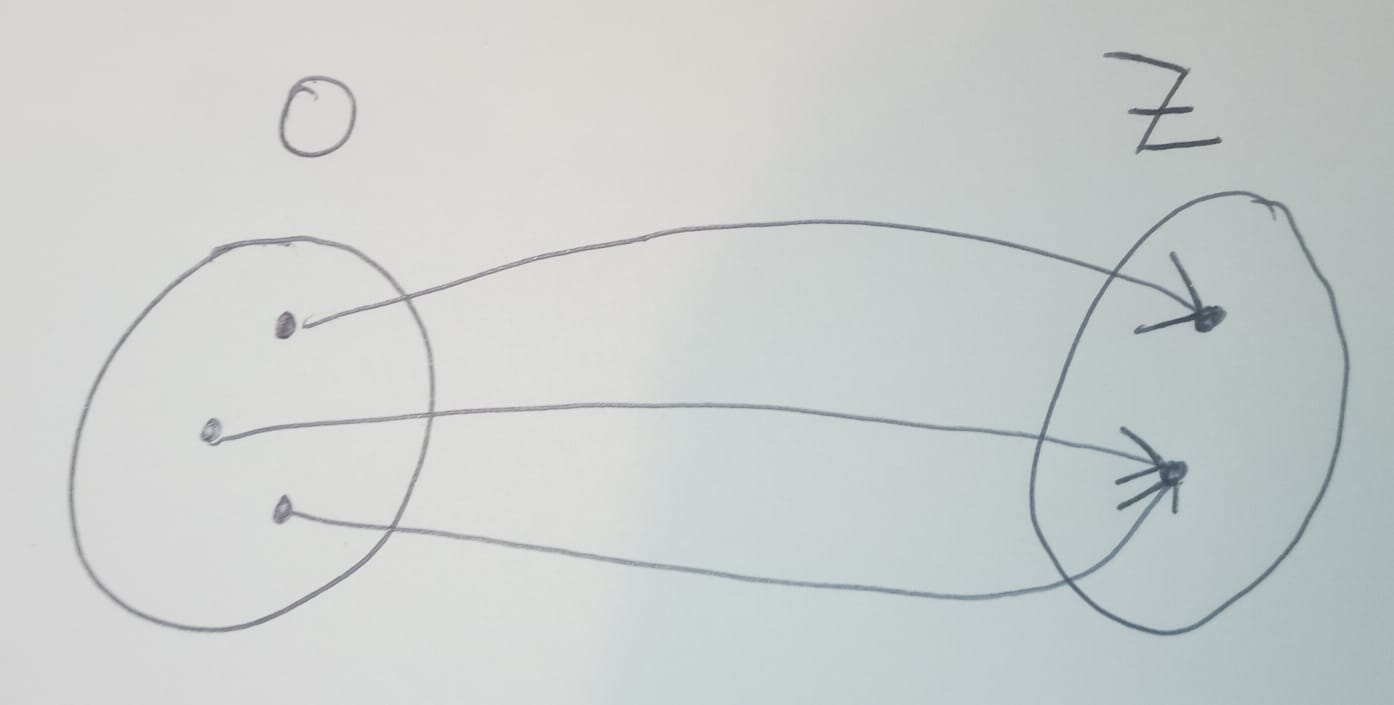
\includegraphics[width=0.5\linewidth]{2MathematicalFramework/Images/inference_process_O_to_Z.jpeg}
	\caption{
		An example of how an inference process $h: O \to Z$ sends each observation state in $O$ to a representation state in $Z$.
		Note how it is possible for two distinct observation states to produce the same representation state.
	}
	\label{fig:inference_process_O_to_Z}
\end{figure}

\newthought{We can combine} $b$ and $h$ to form a mapping
\begin{equation}
\begin{aligned}
	& f: W \to Z \\
	& \text{such that } f = h \circ b
\end{aligned}
\end{equation}
that describes the process of the agent obtaining and processing information about the world.

\begin{figure}[H]
	\centering
	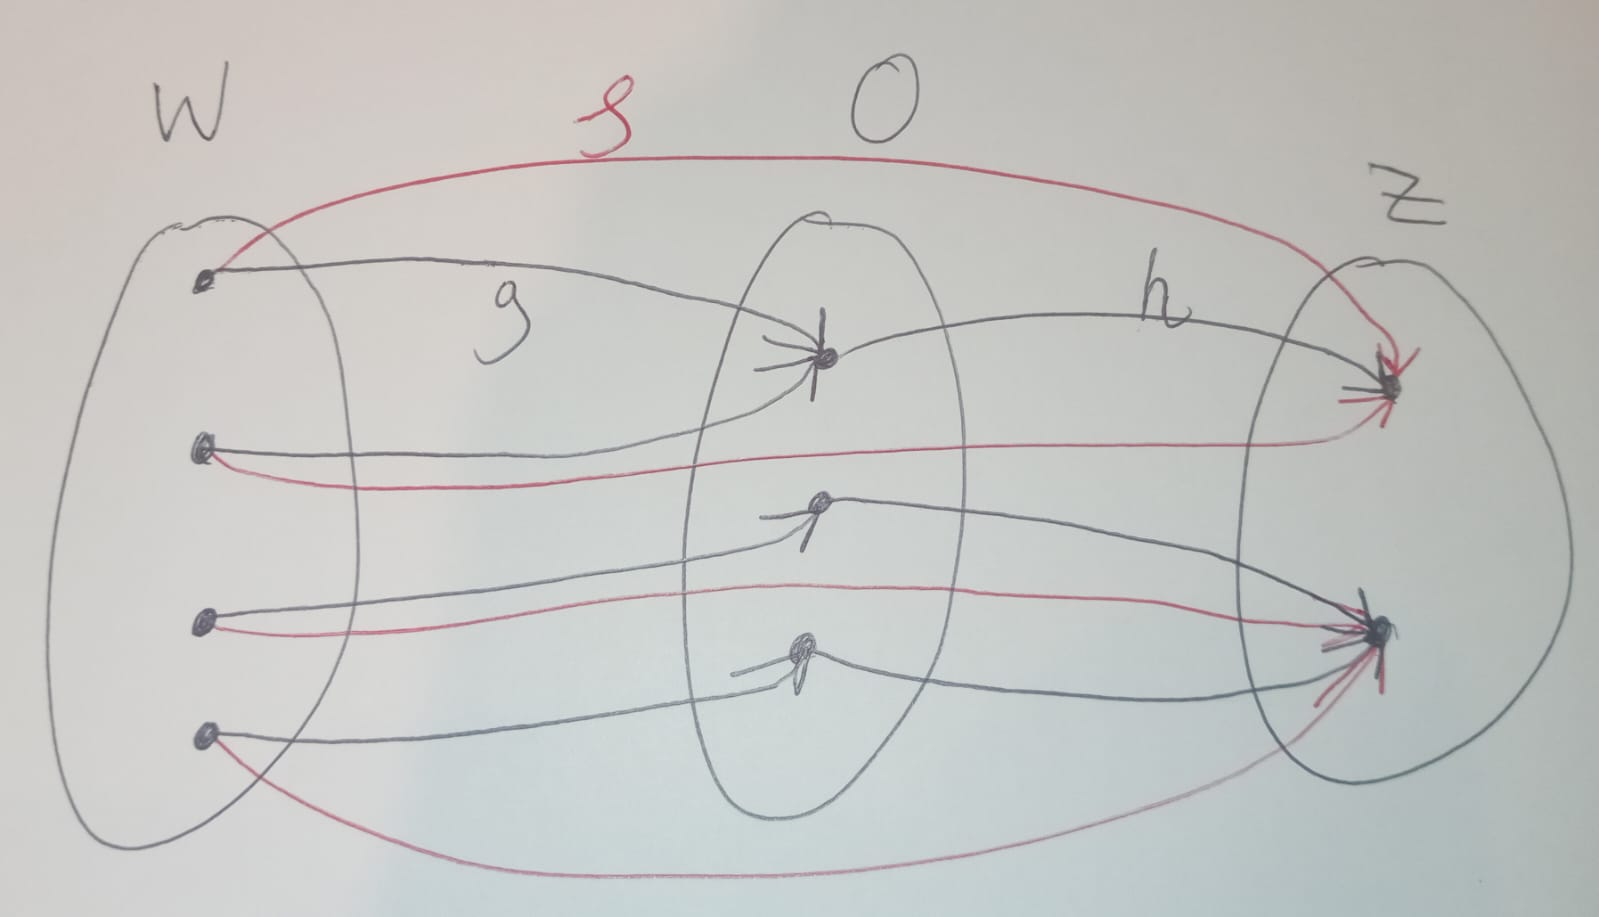
\includegraphics[width=0.5\linewidth]{2MathematicalFramework/Images/W_to_Z.jpeg}
	\caption{
		An example of the map $f: W \to Z$ sends each world state in $W$ to a representation state in $Z$.
		\draftnote{blue}{awjdean}{$g$ should be $b$.}
	}
	\label{fig:W_to_Z}
\end{figure}


\begin{propositionE}[][normal]
	For agents with ideal sensors, the map $f$ is bijective.
\end{propositionE}
\begin{proofE}
	\draftnote{blue}{awjdean}{Proof that $f$ is bijective if agent ideal sensors.
	1. Prove $b$ bijective.
	2. Prove $h$ bijective.
	3. Composition of two bijective maps is also a bijective map.
}
\end{proofE}

\draftnote{purple}{To do (after submission)}{
Figure showing $W$ to $O$ to $Z$ mappings for an agent with \textbf{ideal sensors}.
}

%%%%%%%%%%%%%%%%%%%%%%%%%%%%%%%%%%%%%%%%
\draftnote{red}{DIVIDER}{}


%%%%%%%%%%%%%%%%%%%%%%%%%%%%%%%%%%%%%%%%%%%%%%
\subsection{Our approach to studying an agent's learning}
\draftnote{blue}{Consider}{Move this up ?}

\newthought{We propose that} there are two approaches for studying the learning of an agent:
\begin{enumerate}
	\item we can study the learning process of the agent itself (i.e., what happens at each step of the learning process;
	\item we can study what we believe the end result of the agent's learning process should be.
\end{enumerate}
Our work focuses on approach (2).

\newthought{We assume that} the best representation of the worlds we study should mirror the relevant structure of the worlds in the structure of the agent's representation; this means the end result of the agent's learning process should be the relevant structure of the world being present in the structure of the agent's representation of the world.

\begin{propositionE}[][normal]
	The representation 'world' should be isomorphic to a subworld of $\mathscr{W}$.
\end{propositionE}
\begin{proofE}
	\draftnote{blue}{awjdean}{Not sure about this}
	\draftnote{green}{Consider}{Is this actually an assumption ?}
\end{proofE}

By initially studying the structure of the worlds themselves, rather than structure of an agent's representation, we can simplify the problem we are tackling since we no longer have to consider each step of the learning process; this provides the opportunity to generalises our results somewhat; results proven about the structure of an agent's representation at the end of the learning process could be agnostic to the learning algorithm\footnote{
This would be the case if the learning algorithm was path independent.
}

Additonally, it might be the case

For example, if we prove that the structure of the world does not obey certain conditions then we might be able to show that this is true no matter the process used for learning
\draftnote{blue}{awjdean}{Flesh this out a bit more - talk about learning equilibria ?
We assume that when learning reaches an equilibirum state, that the dynamics of the representation states are isomorphic to a subworld of $\mathscr{W}$.
}
.

\draftnote{red}{UP NEXT}{
\begin{enumerate}
	\item Define the representation multigraph.
	\item We assume that the representation multigraph is ismorphic to a subworld of $\mathscr{W}$ at the end of the learning process
	\begin{itemize}
		\item (footnote) Or when learning equilibirum reached.
	\end{itemize}
\end{enumerate}
}


%%%%%%%%%%%%%%%%%%%%%%%%%%%%%%%%%%%%%%%%%%%%%%%%%%%%%%%%%%%%
\draftnote{red}{DIVIDER}


\draftnote{green}{To do}{
	\begin{enumerate}
		\item Sensory perception in an agent.
		      \begin{compactitem}
			      \item Look at Higgins distribution set up.
			      \item Cones figure - cone in $W$ leading to a single observation in $O$ - put in later discussion.
			      \item If the agent has ideal sensors (i.e., there is no noise from the sensors) the number of possible observation states is less than or equal to the number of world states (i.e., $|O| \leq |W|$) - put this should later with a proof.
		      \end{compactitem}
		\item Learning.
		      \begin{compactitem}
			      \item Brief discussion about scenarios where you can have $b(w_{1}) = b(w_{2})$ but $h(b(w_{1})) \neq h(b(w_{2}))$ - say we'll discuss this in more detail later.
			      \item Proof that the structure of an agent's representation should mirror the structure of the agent's representation for an agent with ideal sensors.
		      \end{compactitem}
	\end{enumerate}
	\textbf{Small things:}
	\begin{enumerate}
		\item Environment vs world.
		\item Mention at start of Agents section that we use a mix of papers for inspiration for our agent: Agent as a Markov blanker paper, Higgins, Caselles-Dupre.
		\item World states as a distribution - see Higgins.
		\item \textbf{References:}
		      \begin{enumerate}
			      \item Agent as a Markov blanket: \url{https://www.researchgate.net/figure/The-structure-of-a-Markov-blanket-A-Markov-blanket-highlights-open-systems-exchanging_fig1_343643283}
		      \end{enumerate}
	\end{enumerate}
	\textbf{Implemented notes:}
	\begin{enumerate}
		\item Do the 'sensory states' in the Markov Blanket represent different observation states in $O$ or different sensors ? They represent different observation states - need to make my formalism consistent. \textbf{Use $o$ for observation states.}
		\item Sensors can mean real-world sensors or virtual inputs (e.g., in a software agent).
	\end{enumerate}
}

%%%%%%%%%%%%%%%%%%%%%%%%%%%%%%%%%%%%%%%%%%%%%%%%%%%%%%%%%%%%%%%%%%%
\section{Actions of agents}

In this section, we define the actions of agents as collections of transformations that are labelled by their associated action.
We then define some relevant properties of these actions.

\draftnote{red}{DIVIDER}{}
\draftnote{blue}{Note}{
	Need to consider $\hat{D}_{A}$ instead of $\hat{D}$ when looking at reachable worlds due to the actions of an agent.
}

\draftnote{red}{Include}{
\begin{enumerate}
    \item [Mention] Actions can be represented as tuples of their unique compositions of minimum actions.
    \item Define operator $\operatorname{Seq}: \hat{A}^{\ast} \to \hat{A}^{(n)}$ that sends an action to its tuple of minimum actions.
    \begin{itemize}
        \item $\operatorname{Seq}$ is a bijective mapping because each action has a unique minimum action tuple.
    \end{itemize}
    \item (after introducing $\bot$)
		Say something about how if we say $a \ast w$ is defined we mean $a \ast w \neq \bot$.
\end{enumerate}
}

\draftnote{green}{Include}{
	\begin{enumerate}
		\item \textbf{Figures:}
		      \begin{itemize}
			      \item Diagram showing what $W$, $Z$, $A$, $w$, $z$, $a$ are.
		      \end{itemize}
	\end{enumerate}
}

\draftnote{red}{DIVIDER}{}


%%%%%%%%%%%%%%%%%%%%%%%%%%%%%%%%%%%%%%%%%%%%%%%%%%%%%%%%%%%%%%%%%%%
\subsection{Actions as collections of labelled transformations}

\draftnote{red}{To do}{
\begin{enumerate}
	\item $\mathscr{W}_{A}$ is a labelled multidigraph.
	\item 
\end{enumerate}
}


\begin{postulate}
	Actions are collections of labelled tranformations.
\end{postulate}

Consider a set $\hat{A}$ called the set of \emph{minimum actions} of an agent, where $\hat{A} = \{1, a_{1}, a_{2}, \dots, a_{n}\}$.

We now take the Kleene star operator of $\hat{A}$ \footnote{
	$\hat{A}^{\ast} = \{ \varepsilon \} \cup \{ (a_1, a_2, \dots, a_n) \mid a_i \in \hat{A}, \, n \in \mathbb{N} \}$.
} to get the set of all possible finite sequences formed from elements of $\hat{A}$, including the empty sequence, which we denote by $\varepsilon$.
We call $\hat{A}^{\ast}$ the set of \emph{actions of the agent}.

We define a composition operator
\begin{equation}
	\circ: \hat{A}^{\ast} \times \hat{A}^{\ast} \to \hat{A}^{\ast}
\end{equation}
such that $(a_1, a_2, \dots, a_n) \in \hat{A}^{\ast}$ can be written as $a_1 \circ a_2 \circ \dots \circ a_n$.

\begin{definition}[Notation block]
	Sometimes we write compositions like $a_1 \circ a_2 \circ \dots \circ a_n$ as $a_1 a_2 \dots a_n$.
\end{definition}

The operator $\circ$ is closed under the definition of the Kleene star operator.

\paragraph{Properties of the empty sequence $\varepsilon$.}
\begin{enumerate}
	\item \textbf{Uniqueness:} There is only one empty sequence $\varepsilon$.
	\item \textbf{Identity element for concatenation:} the empty sequence $\varepsilon$ serves as an identity element for concatenation of sequences:
	      $\varepsilon \circ a = a \circ \varepsilon = a$ for all $a \in \hat{A}^{\ast}$.
	\item \textbf{Length:} The empty sequence $\varepsilon$ has a length of zero (i.e., $|\varepsilon| = 0$).
\end{enumerate}

\paragraph{Linking actions with transformations.}
We now want to link our set of actions to the transformations of the world that would occur if an agent performed each action while in a current world state.
We do this by first labelling transformations in the set $D$ of transformations that are caused by minimum actions with the elements of $\hat{A}$, and then using those labellings to label other transformations in $D$ with the elements of $\hat{A}^{\ast}$ by considering how the elements of $\hat{A}$ combine to form the elements of $\hat{A}^{\ast}$.

Consider a set $\hat{D}_{A} \subset D$, where $1_{w} \in \hat{D}_{A}$ for all $w \in W$; we call $\hat{D}_{A}$ the set of \textit{minimum action transformations}.
We define a labelling map $\hat{l}: \hat{D}_{A} \to \hat{A}$ such that $\hat{l}$ satisfies the following conditions:
\begin{enumerate}
	\item \textbf{Uniqueness condition.}
	      Any two distinct atomic transformations leaving the same world state are labelled with different actions:
	      \begin{equation}
		      \text{If } s(d) = s(d'), \text{ then } \hat{l}(d) \neq \hat{l}(d') \quad \text{for any } d, d' \in \hat{D}_{A}.
	      \end{equation}

	\item \textbf{Identity condition.}
	      Trivial transformations, $1_{w}$ for all $w \in W$, are mapped to the empty sequence $\varepsilon$:
	      \begin{equation}
		      \hat{l}(1_{w}) = \varepsilon \quad \text{for all } w \in W.
	      \end{equation}
\end{enumerate}

So, for any world $\mathscr{W} = (W, \hat{D})$, there is a subworld $\mathscr{W}_{A} = (W, \hat{D}_{A})$.
In the same way as we did in \cref{sec:A mathematical treatment of worlds and their transformations} to get $D$ from $\mathscr{W}$, we take the set of all finite directed walks in $\mathscr{W}_{A}$ and denote it by $D_{A}$; the elements of $D_{A}$ are called \emph{transformations due to the actions of the agent}.
As before, we extend $\hat{s}$ and $\hat{t}$ to $s$ and $t$ respectively\footnote{
	We can use $s$, $t$ instead of having to define sub maps $s_{A}$ and $t_{A}$ because $s$ and $t$ act on the elements of $D$ and $D_{A}$ is just $D$ with some elements removed.
	If we wanted to define such maps $s_{A}$ and $t_{A}$ they would be restrictions of the maps $s$ and $t$ to the set $D_{A}$.
	\draftnote{blue}{awjdean}{
		- Put this as a footnote for the definition of subworlds?
		does this slightly alter the definition of subworld ?
	}
}.

We extend the map $\hat{l}$ to the map $l: D_{A} \to \hat{A}^{\ast}$ such that:
if $d = \hat{d}_{n} \circ ... \circ \hat{d}_{1}$ then $l(d) = \hat{l}(\hat{d}_{n}) ... \hat{l}(\hat{d}_{1})$.
The extended map $l$ now satisfies the following conditions:
\begin{enumerate}
	\item Any two distinct transformations leaving the same world state are
	      labelled with different actions.
	      \begin{action_condition}[Uniqueness]\label{actcon:action_gives_single_outcome}
		      For any $d,d' \in D_{A}$ with $s(d)=s(d')$, $l(d) \neq l(d')$.
	      \end{action_condition}

	\item Trivial transformations, $1_{w}$ for all $w \in W$, are mapped to the empty sequence $\varepsilon$:
	      \begin{action_condition}[Identity]\label{actcon:trivial_transformations_mapped_to_empty_sequence}
		      $l(1_{w}) = \varepsilon$ for all $w \in W$.
	      \end{action_condition}

	\item Transformations are labelled consistently with the sequence of labels corresponding to their constituent atomic transformations.
	      \begin{action_condition}[Composition consistency]\label{actcon:composition_consistency}
		      If $d = \hat{d}_{n} \circ ... \circ \hat{d}_{1}$ then $l(d) = \hat{l}(\hat{d}_{n}) ... \hat{l}(\hat{d}_{1})$ for all $d \in D_{A}$ and for all $\hat{d_{1}}, \dots , \hat{d_{n}} \in \hat{D}_{A}$.
	      \end{action_condition}
\end{enumerate}

For $d \in D_{A}$ with $s(d) = w$, $t(d) = w'$ and $l(d) = a$, we will often denote $d$ by $d: w \xrightarrow{a} w'$.

A summary of the procedure we've taken to label the transformations of a world $\mathscr{W}$ that are due to the actions of an agent is given by \cref{fig:action_labelling_procedure}.

\begin{figure}
	\centering
	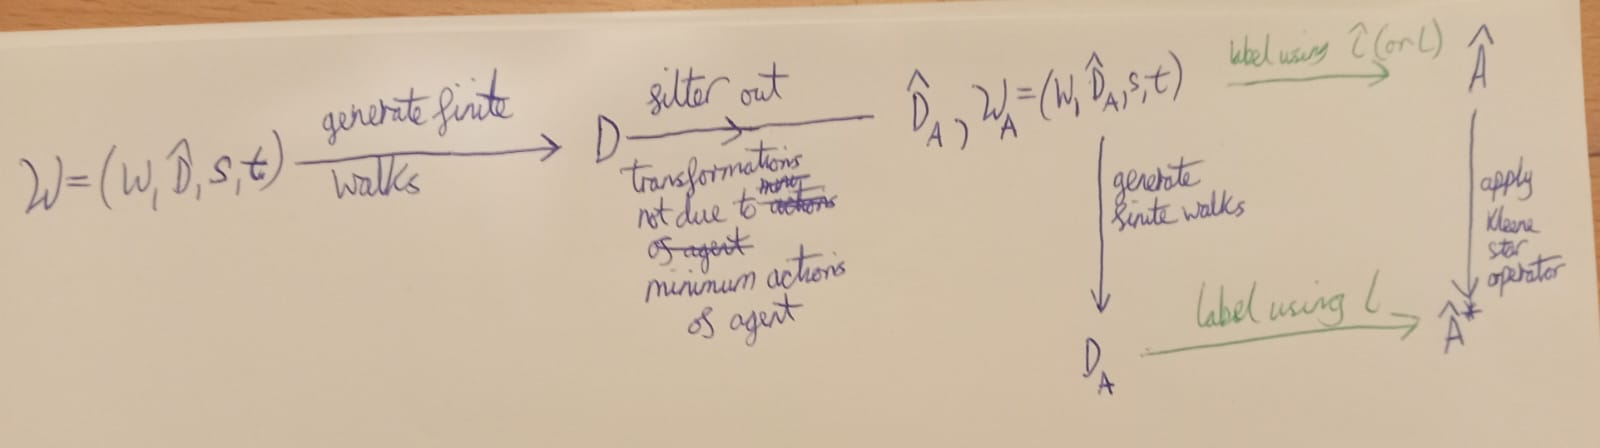
\includegraphics[width=\linewidth]{2MathematicalFramework/Images/action_labelling_procedure.jpeg}
	\caption{Procedure for labelling the transformations of the world with their associated action.}
	\label{fig:action_labelling_procedure}
\end{figure}


\paragraph{Effect of actions on world states.}
\draftnote{blue}{awjdean}{Define $\hat{\ast}$ first then extend to $\ast$ - we need $\hat{\ast}$ for Cayley algorithms.}
Unlike transformations, which are tied to individual world states, actions can have different outcomes when applied to different world states.
For example, it could be the case that applying the action $a$ followed by the action $b$ on a world state $w_{1}$ gives back the original world state, while applying $a$ followed by $b$ on world state $w_{2}$ could give a different world state $w_{3}$ - the action sequence $ba$ produces the original world state when applied to certain world states (e.g., $w_{1}$), but produces a world state that is not the original world state when applied to other world states (e.g., $w_{2}$).
Due to this behaviour, we need a way to describe how actions change world states.
We define the \emph{effect of an action $a \in \hat{A}^{\ast}$ on a world state $w \in W$} as
\begin{equation}
	\ast: \hat{A}^{\ast} \times W \to W
\end{equation}
such that
\begin{enumerate}
	\item if there exists a $d: w \xrightarrow{a} t(d)$, then $a \ast w = t(d)$; and
	\item if there does not exist a $d: w \xrightarrow{a} t(d)$, then we say that $a \ast w$ is \emph{undefined}.
\end{enumerate}


The effect of actions on world states is well-defined due to \cref{actcon:action_gives_single_outcome} \draftnote{blue}{awjdean}{Prove this explicitly?}.

The compatibility of $\ast$ and $\circ$ is given by:
\begin{equation}\label{eqn:circ_ast_compatibility}
	(a' \circ a) \ast w = a' \ast (a \ast w) \quad \text{for any $a, a' \in \hat{A}^{\ast}$ and $w \in W$}
\end{equation}
\footnote{
	This follows naturally from the composition consistency property on the labelling map $l$:
	If $d_{1}: w \xrightarrow{a} w'$ and $d_{2}: w' \xrightarrow{a'} w''$, then $d_{2} \circ d_{1}: w \xrightarrow{a' \circ a} w''$.
	By the definition of $\ast$, $a * w = t(d_{1})$, $a' \ast (a \ast w) = t(d_{2})$, and $(a' \circ a) \ast w = t(d_{2} \circ d_{1})$.
	Therefore, since $d_{2} \circ d_{1}$ has the label $a' \circ a$, we see that $(a' \circ a) \ast w = a' \ast (a \ast w)$.
}

This means we can apply the minimum actions that make up an action to world states individually:

if $a = \hat{a}_{k}...\hat{a}_{1}$, then
\begin{align}
	a \ast w & = (\hat{a}_{k} \dots \hat{a}_{1}) \ast w                                       \\
	         & = (\hat{a}_{k} \dots \hat{a}_{2}) \ast (\hat{a}_{1} \ast w)                    \\
	         & = (\hat{a}_{k} \dots \hat{a}_{3}) \ast (\hat{a}_{2} \ast (\hat{a}_{1} \ast w)) \\
	         & = \dots
\end{align}

We can also split actions into short sequences of actions and apply those:

if $a = \hat{a}_{k}...\hat{a}_{1}$, then
\begin{align}
	a \ast w & = (\hat{a}_{k} \dots \hat{a}_{3}) \ast (\hat{a}_{2} \ast (\hat{a}_{1} \ast w))  \\
	         & = (\hat{a}_{k} \dots \hat{a}_{3}) \ast ((\hat{a}_{2} \circ \hat{a}_{1}) \ast w) \\
	         & = \dots
\end{align}

\Cref{eqn:circ_ast_compatibility} means that $\ast$ is an \emph{action} of the algebra $(\hat{A}^{\ast}, \circ)$ on the set $W$ \footnote{
	The action of an algebra is different to the actions of an agent.
	Yes, it's confusing!
}.


%%%%%%%%%%%%%%%%%%%%%%%%%%%%%%%%%%%%%%%%%%%%%
\subsection{Actions as (partial) functions.}

Consider all the transformations that are labelled by a particular action $a \in \hat{A}^{\ast}$.
Together these transformations form a partial function $f_{a}: W \to W$ because for any $w \in W$ either $a \ast w$ is undefined or $a \ast w$ is defined and there is a unique world state $w' \in W$ for which $a \ast w = w'$ (from \cref{actcon:action_gives_single_outcome}).
Each of the transformations labelled by the action $a$ is an assignment of $f_{a}$ to one of the world states in $W$ ($f_{a}(w) \mapsto a \ast w = w'$).

Formally, we can curry\footnote{Currying allows us to transform an operation with multiple arguments into a collection of functions with single arguments by fixing all but one of the operation's arguments.} the action effect operator $\ast : \hat{A}^{\ast} \times W \to W$
\begin{equation}
	\textit{Curry}: (\ast: \hat{A}^{\ast} \times W \to W) \to (f_{a}: W \to W)
\end{equation}
to obtain a collection of (partial) functions
\begin{equation}
	\mathcal{T}_{\hat{A}^{\ast}} = \{f_{a}: W \to W \mid f_{a}(w) = a \ast w \text{ where defined, for each } a \in \hat{A}^{\ast} \}
\end{equation}

These functions $f_{a}$
\begin{enumerate}
	\item are not generally surjective because for a given $w \in W$ there is not necessarily a transformation $d \in D$ with $l(d) = a$ and $t(d) = w$ \draftnote{blue}{awjdean}{Illustrative diagram}.

	\item are not generally injective because it is possible to have an environment where $f_{a}(w)=f_{a}(w')$ for some $w \in W$ different from $w' \in W$ \draftnote{blue}{awjdean}{Illustrative diagram}.
\end{enumerate}

\draftnote{blue}{Footnote}{
	We can also reproduce these functions using the formalism given by \autocite{caselles2019symmetry}, which describes the dynamics of the world in terms of a multivariate function $f: A \times W \to W$.
	If we let $f: A \times W \to W$ be the dynamics of the environment then the transformation caused by an action $a \in A$ on a world state $w \in W$ (where $a \ast w$ is defined) is given by $(a,w) \mapsto f(a,w) = a \ast w$. \draftnote{blue}{awjdean}{Put stuff like this in a separate "Other formalisms described using our formalism" section after Reproducing SBDRL ?}
}

%%%%%%%%%%%%%%%%%%%%%%%%%%%%%%%%%%%%%%%
\subsection{Reachable subworlds due to the actions of an agent}

\draftnote{blue}{To do}{
	Something (earlier) about how we need to specify $\hat{D}_{A}$ (you could have a transformation in $\hat{D}_{A}$ that's not in $\hat{D}$) - perhaps bundle this into world-agent pair.
}

To define reachable subworlds due to the actions of an agent, we take the reachable subworlds definition and replace $\hat{D}$ with $\hat{D}_{A}$.
For a world $\mathscr{W} = (W, \hat{D}, \hat{s}, \hat{t})$ containing an agent with minimum actions $\hat{A}$ and minimum action transformations $\hat{D}_{A}$,
\begin{align}
	 & W^{\hat{A}\to}(w) := \{ w' \in W \mid \text{there exists} \; d \in D_{A} \; \text{with} \; d: w \to w' \}                                                                 \\
	 & \hat{D}_{A}^{\hat{A}\to}(w) := \{ \hat{d} \in \hat{D}_{A} \mid s(\hat{d}) \in W^{\hat{A}\to}(w) \; \text{and} \; t(\hat{d}) \in W^{\hat{A}\to}(w) \}                      \\
	 & \mathscr{W}^{\hat{A}\to}(w) := (W^{\hat{A}\to}(w), \hat{D}_{A}^{\hat{A}\to}(w), \hat{s} \big|_{\hat{D}_{A}^{\hat{A}\to}(w)}, \hat{t} \big|_{\hat{D}_{A}^{\hat{A}\to}(w)})
\end{align}
where $W^{\hat{A}\to}(w)$ is the set of world states that are reachable from the world state $w \in W$ using the actions of the agent, $\hat{D}_{A}^{\hat{A}\to}(w)$ is the set of atomic transformations that are reachable from $w$ using the actions of the agent, and $\mathscr{W}^{\hat{A}\to}(w)$ is the reachable subworld of $\mathscr{W}$ from $w$ using the actions of the agent.
The natural reachable subworld due to the actions of the agent is denoted by $\mathscr{W}^{\hat{A}\to}(w^{*})$.


%%%%%%%%%%%%%%%%%%%%%%%%%%%%%%%%%%%%%%%
\subsection{From partial to total}

We will now turn our partial functions into total functions by adding a new state $\bot$ to our set $W$ of world states, where $\bot$ represents the \emph{undefined state}\footnote{
	This technique for turning partial functions into total functions is used in functional programming languages like Haskell \draftnote{blue}{awjdean}{Reference.}.
}.
\begin{equation}
	W^{\bot} = W \cup \{ \bot \}
\end{equation}

We also extend the effect $\ast : \hat{A}^{\ast} \times W \to W$ of actions on world states to $\ast^{\bot} : \hat{A}^{\ast} \times W^{\bot} \to  W^{\bot}$ so that if $a \ast w$ is defined then it remains the same as before, but if $a \ast w$ is undefined, then we set $a \ast^{\bot} w$ equal to our undefined state $\bot$:
\begin{align}
	 & \ast^{\bot} : \hat{A}^{\ast} \times W^{\bot} \to  W^{\bot} \quad\text{such that} \\
	 & a \ast^{\bot} w =
	\begin{cases}
		t(d) & \text{if, for $d \in D_{A}$, } d : w \xrightarrow{a} t(d) \text{ exists}, \\
		\bot & \text{otherwise.}
	\end{cases}
\end{align}
\footnote{
	Note that we have:
	\begin{equation}
		a \ast^{\bot} \bot = \bot \quad \text{for all $a \in \hat{A}^{\ast}$}
	\end{equation}
	which means that $\bot$ acts as an absorbing element for $\ast^{\bot}$.
}

We can also augmented our set $D_{A}$ of transformations to a set $D_{A}^{\bot}$, which includes the new transformations that send world states to $\bot$, so that we have underlying transformations that reflect the behaviour of $\ast^{\bot}$.
First, we define the set $\Delta^{\bot}$ of new transformations that terminate at $\bot$, which includes transformations for $a \ast^{\bot} \bot$:
\begin{alignat}{2}
	U             & {}={} &  & \{ (a,w) \in \hat{A}^{\ast} \times W \mid \not\exists (d: w \xrightarrow{a} t(d)) \in D_{A} \} \\
	\Delta^{\bot} & {}={} &  & \{ d^{\bot}: w \xrightarrow{a} \bot \mid (a, w) \in U \}                                       \\
	              &       &  & \cup \{ d^{\bot}: \bot \xrightarrow{a} \bot \text{ for all $a \in \hat{A}^{\ast}$} \}
\end{alignat}

\draftnote{blue}{awjdean}{Change symbol for temporary set $U$ ? - have a symbol that is used for a temporary thing that is never used again ?}
\begin{equation}
	D_{A}^{\bot} = D \cup \Delta^{\bot}
\end{equation}

Now we can extend our action labelling map $l: D_{A} \to \hat{A}^{\ast}$ to include our new $\bot$-terminating transformations:
\begin{align}
	 & l^{\bot} : D_{A}^{\bot} \to \hat{A}^{\ast} \quad\text{such that} \\
	 & l^{\bot}(d) =
	\begin{cases}
		l(d) & \text{if $d \in D_{A}$},                                            \\
		a    & \text{if $d \in \Delta^{\bot}$ and $d: s(d) \xrightarrow{a} \bot$.}
	\end{cases}
\end{align}

To simplify notation, we will use $W$, $\ast$, $D_{A}$, and $l$ to denote $W^{\bot}$, $\ast^{\bot}$, $D_{A}^{\bot}$, and $l^{\bot}$ respectively unless we want to explicitly differentiate between the use of $W$, $\ast$, $D_{A}$, and $l$ vs $W^{\bot}$, $\ast^{\bot}$, $D_{A}^{\bot}$, and $l^{\bot}$.

\draftnote{green}{To do}{
	\begin{enumerate}
		\item Footnote about potential loss of information about why an action was undefined  (e.g., if two distinct actions are undefined on the same state $w$ then their effects are indistinguishable after $\bot$ is reached because $\bot$ is absorbing - in this cases we could introduce $\bot_{1}, \bot_{2}, \bot_{3} \dots$ to separate out different "types" of undefined.
	\end{enumerate}
}

%%%%%%%%%%%%%%%%%%%%%%%%%%%%%%%%%%%%%%%%%
\subsection{$(\hat{A}^{\ast}, \circ)$, $\mathcal{T}_{\hat{A}^{\ast}}$, and $(\hat{A}^{\ast}, \circ, \ast)$}

There are three notable structures which we will explore in this section: $(\hat{A}^{\ast}, \circ)$, $\mathcal{T}_{\hat{A}^{\ast}}$, and $(\hat{A}^{\ast}, \circ, \ast)$.

%%%%%%%%%%%%%%%%%%%%%%%%%%%%%%%%%%%%%%%%%
\paragraph{$(\hat{A}^{\ast}, \circ)$.}
$(\hat{A}^{\ast}, \circ)$ is the free monoid generated by the set $\hat{A}$, where $\circ$ acts like the concatenation of strings.
This means there are no relations between the generators in $\hat{A}$ apart from the associativity and identity required for $(\hat{A}^{\ast}, \circ)$ being a monoid, and so $(\hat{A}^{\ast}, \circ)$ provides maximum flexibility in constructing elements\footnote{Note that the structure of $(\hat{A}^{\ast}, \circ)$ is unaffected by the effect $\ast$ of actions on world states.}.

\draftnote{blue}{awjdean}{Proof that $(\hat{A}^{\ast}, \circ)$ is closed ?}
\begin{proposition}
	$(\hat{A}^{\ast}, \circ)$ is a monoid.
\end{proposition}
\begin{proof}
	\begin{enumerate}
		\item \textbf{Associativity.}
		      $\circ$ is associative for all $a \in \hat{A}^{\ast}$
		      \draftnote{blue}{awjdean}{Prove this explicitly.}
		\item \textbf{Identity element.}
		      The empty action $\varepsilon$ acts as the identity element:
		      \begin{equation}
			      \varepsilon \circ a = a \quad \text{and} \quad a \circ \varepsilon = a \quad \text{for all } a \in \hat{A}^{\ast}.
		      \end{equation}
	\end{enumerate}
\end{proof}

%%%%%%%%%%%%%%%%%%%%%%%%%%%%%%%%%%%%%%%%%
\paragraph{$\mathcal{T}_{\hat{A}^{\ast}}$.}
Now we have introduced the undefined state $\bot$, the set $\mathcal{T}_{\hat{A}^{\ast}}$ is a set of (total) functions $f_{a}: W \to W$ with one $f_{a}$ for each action $a \in \hat{A}^{\ast}$ \footnote{
Making the $\bot$'s explicit, $\mathcal{T}_{\hat{A}^{\ast}}$ is now defined as:
\begin{equation}
	\begin{aligned}
		\mathcal{T}_{\hat{A}^{\ast}} = \{ & f_{a}: W^{\bot} \to W^{\bot} \mid                                \\
		                                  & f_{a}(w) = a \ast^{\bot} w \text{ for $a \in \hat{A}^{\ast}$} \}
	\end{aligned}
\end{equation}
}.

\begin{proposition}\label{prp:T_is_monoid}
	$\mathcal{T}_{\hat{A}^{\ast}}$ is a monoid under composition $\cdot: \mathcal{T}_{\hat{A}^{\ast}} \times \mathcal{T}_{\hat{A}^{\ast}} \to \mathcal{T}_{\hat{A}^{\ast}}$ of functions such that:
	\begin{equation}
		f_{a' \circ a} = f_{a'} \circ f_{a}
	\end{equation}
\end{proposition}
\begin{proof}
	\begin{enumerate}
		\item \textbf{Associativity.}
		      Associativity of the composition of the partial functions $f_{a}$ follows from the associativity of $\circ: \hat{A}^{\ast} \times \hat{A}^{\ast} \to \hat{A}^{\ast}$:
		      \begin{align}
			      (f_{a''} \cdot f_{a'}) \cdot f_{a} & = f_{a'' \circ a'} \cdot f_{a}       \\
			                                         & = f_{(a'' \circ a') \circ a}         \\
			                                         & = f_{a'' \circ (a' \circ a)}         \\
			                                         & = f_{a''} \cdot f_{a' \circ a}       \\
			                                         & = f_{a''} \cdot (f_{a'} \cdot f_{a})
		      \end{align}
		\item \textbf{Identity element.}
		      The function $f_{\varepsilon}$ correspondence to the empty action $\varepsilon$ is the identity function\draftnote{blue}{awjdean}{Make this more explicit?}:
		      \begin{equation}
			      f_{\varepsilon}(w) = \varepsilon \ast w = w \quad \text{for all $w \in W$}
		      \end{equation}
	\end{enumerate}
\end{proof}

There exists a monoid homomorphism\footnote{
$\phi$ arises directly due to the \emph{universal property of free monoids}.
We take a mapping $a \mapsto f_{a}$ that assigns each minimum action $a \in \hat{A}$ to its corresponding effect function $f_{a}$.
Then, by the universal property of free monoids, $a \mapsto f_{a}$ uniquely extends to a monoid homomorphism $\phi : \hat{A}^{\ast} \to \mathcal{T}_{\hat{A}^{\ast}}$ that preserves the monoid structure.
\draftnote{blue}{awjdean}{Expand on this ?}
} from $(\hat{A}^{\ast}, \circ)$ to $\mathcal{T}_{\hat{A}^{\ast}}$:
\begin{equation}
	\phi : \hat{A}^{\ast} \to \mathcal{T}_{\hat{A}^{\ast}} \quad\text{defined by $\phi(a) = f_{a}$}
\end{equation}
that preserves the monoid structure
\begin{align}
	 & \phi(a' \circ a) = f_{a' \circ a} = f_{a'} \cdot f_{a} = \phi(a') \cdot \phi(a) \\
	 & \phi(\varepsilon) = f_{\varepsilon}
\end{align}

\draftnote{blue}{awjdean}{$\mathcal{T}_{\hat{A}^{\ast}}$ is an action monoid.}

Each function $f_{a}$ precisely represents the effect of an action $a \in \hat{A}^{*}$ on all possible world states.

Other properties of $f_{a} \in \mathcal{T}_{\hat{A}^{\ast}}$:
\begin{enumerate}
	\item \textbf{Not generally invertible.}
	      There may not exist a function $f_{a}^{-1}$ such that $f_{a}^{-1} \circ f_{a} = f_{a} \circ f_{a}^{-1} = f_{\varepsilon}$.
	\item \textbf{Not necessarily injective.}
	      It is possible for a function $f_{a}$ to map different world states to the same world state (i.e., it is possible to have $f_{a}(w) = f_{a'}(w)$).
	\item \textbf{Not necessarily surjective onto $W$.}
	      It is possible for there to be a world state that is not reachable through a function $f_{a}$ (i.e., it is possible for a $w \in W$ to exist such that there is no $w' \in W$ where $f_{a}(w') = w$ for some $a \in \hat{A}^{\ast}$).
\end{enumerate}

\draftnote{blue}{awjdean}{Note about the structure of $\mathcal{T}_{\hat{A}^{\ast}}$ is $\bot$ not introduced.}
\draftnote{blue}{awjdean}{$\mathcal{T}_{\hat{A}^{\ast}}$ may not be closed under composition due to partiality and redundancy, and therefore $\mathcal{T}_{\hat{A}^{\ast}}$ is not in general a monoid.}

%%%%%%%%%%%%%%%%%%%%%%%%%%%%%%%%%%%%%%%%%
\paragraph{$(\hat{A}^{\ast}, \circ, \ast)$.}
\begin{proposition}
	$(\hat{A}^{\ast}, \circ, \ast)$ is a monoid action of $\hat{A}^{\ast}$ on the set $W$.
\end{proposition}
\begin{proof}
	\begin{enumerate}
		\item \textbf{Compatibility.}
		      The action effect operator $\ast$ is compatible with the composition operator $\circ$ since:
		      \begin{equation}
			      (a \circ b) \ast w = a \ast (b \ast w) \quad \text{for all } a, b \in A^{\ast}, \, w \in W.
		      \end{equation}

		\item \textbf{Identity action.}
		      The empty action $\varepsilon$ acts as the identity on $W$:
		      \begin{equation}
			      \varepsilon \ast w = w \quad \text{for all } w \in W.
		      \end{equation}

	\end{enumerate}
\end{proof}

\draftnote{blue}{awjdean}{Double check that $(\hat{A}^{\ast}, \circ, \ast)$ is a monoid.}

\draftnote{blue}{Consider}{
	What would the structures be with no $\bot$ use --> Category or partial transformation monoid ?
}

\draftnote{blue}{Consider - Other potentially useful properties of $(\hat{A}^{\ast}, \circ)$}{
	\begin{enumerate}
		\item Any monoid homomorphism from $(\hat{A}^{\ast}, \circ)$ to another monoid is fully determined by its action on the generators $\hat{A}$.
		      \begin{itemize}
			      \item Does this mean that if we change the minimum actions we'll be able to map generators to find out if there's an isomorphism ?
		      \end{itemize}
		\item $(\hat{A}^{\ast}, \circ)$ is closed.
		\item $(\hat{A}^{\ast}, \circ)$ is decidable (i.e., there exists an algorithm that can always provide a correct yes-or-no answer in a finite amount of time).
		      \begin{itemize}
			      \item Operations in Structures: In the context of $(\hat{A}^{\ast}, \circ)$, the questions "Is $s_{1} \circ s_{2} = s_{3}$" or "Does $s$ belong to $\hat{A}^{\ast}$?" are decidable because we can compute the concatenation $s_{1} \circ s_{2}$ and compare it to $s_{3}$, or verify $s$'s construction from the alphabet $\hat{A}$, respectively.
		      \end{itemize}
	\end{enumerate}
}

\draftnote{green}{To do}{
	\begin{enumerate}
		\item Appendix: Why $\hat{A}$ is not necessarily labelling elements of $\hat{D}$ only.
		\item Have I said that $\hat{D}_{A}$ contains $D_{\varepsilon}$ by definition ?
		\item Is $l$ actually a collection of maps $l_{w}$ for each $w \in W$ ? --> endomorphism viewpoint ?
		\item Talk about why we've created action condition 1.
		\item \textbf{Footnote:} difference between the empty action and the no op action.
		\item Say we refer to the empty sequence as the empty action.
		\item \textbf{Mention:} We can use $s$, $t$ instead of having to define sub maps $s_{A}$ and $t_{A}$ because $s$ and $t$ act on the elements of $D$ and $D_{A}$ is just $D$ with some elements removed. - Put this as a footnote for the definition of subworlds; does this slightly alter the definition of subworld ?
		\item \textbf{Mention:} Minimum actions denoted by $\hat{hat}$.
		\item No-op action doesn't always exist.
		      \begin{compactitem}
			      \item Physically, the identity action $1 \in A$ corresponds to the no-op action (\textit{i.e.}, the world state does not change due to this action).
		      \end{compactitem}
		\item \Cref{actcon:action_gives_single_outcome} means that for each $w \in W$, there is a subset of $\hat{D}_{A}$ given by $\{d \mid d \in \hat{D}_{A}\textit{, } s(d)=w\}$; for each of these subsets, the elements of the subset are uniquely labelled (within the subset) by $l$.
		      In other words, the transformations in $D_{A}$ with source $s(d)$ are uniquely labelled by $\hat{l}$ for all $d \in D_{A}$.
		\item Summary
		      \begin{compactitem}
			      \item $a \sim a' \Leftrightarrow f_{a} = f_{a'} \Leftrightarrow \textit{for all } w \in W^{\bot}, \; a \ast w = a' \ast w$.
			      \item $\hat{A}^{\ast}/\sim \; \Leftrightarrow \mathcal{T}$ (set of distinct transformations $W^{\bot} \to W^{\bot}$.
		      \end{compactitem}
	\end{enumerate}
}

\draftnote{blue}{Questions/thoughts that have been answered:}{
	\begin{enumerate}
		\item $A$ is the set of words made from $\hat{A}$ - i.e., the set of finite sequences of elements of $A$, not infinite sequences - infinite sequences make things tricky (apparently).
		\item We want the set $A$ of actions to be the Kleene star operation of $\hat{A}$ ($A = \hat{A}^{\ast}$). $\hat{A}^{\ast}$ includes an empty sequence $\varepsilon$ and our no-op action $1$ as separate sequences; if the no op action is an identity action, then $1 \sim \varepsilon$.
	\end{enumerate}
}

%%%%%%%%%%%%%%%%%%%%%%%%%%%%%%%%%%%%%%%%%%%%%%%%%%%%%%%%%%%%%%%%%%%%%%%%%%%%%%%%%%%%%%%%%%%%%%
\section{
  An example world \texorpdfstring{$\mathscr{W}_{\alpha}$}{}
 }\label{sec:an_example_world}

So far we've seen a lot of definitions and mathematical descriptions, now we will illustrate these ideas through a toy example.
Our chosen toy problem is a $2\times 2$ cyclic grid world $\mathscr{W}_{\alpha}$, where all the transformations in $\mathscr{W}_{\alpha}$ are due to the actions of an agent embodied in the world.

%%%%%%%%%%%%%%%%%%%%%%%%%%%%%%%%%%%%%%%%%%%%%%%%%%%%%%%%%%%%%%%%%%%%%%%%%%%%%%%%%%%%%%%%%%%%%%
\subsection{World states of $\mathscr{W}_{\alpha}$}\label{sec:World states of example}

The world states of $\mathscr{W}_{\alpha}$ are shown in \cref{fig:2x2-cyclical-grid-world-states}.
So, for $\mathscr{W}_{\alpha}$, $W = \{ w_{0}. w_{1}, w_{2}, w_{3} \}$.
\begin{figure}[H]
	\centering
	\begin{subfigure}[b]{0.45\linewidth}
		\centering
		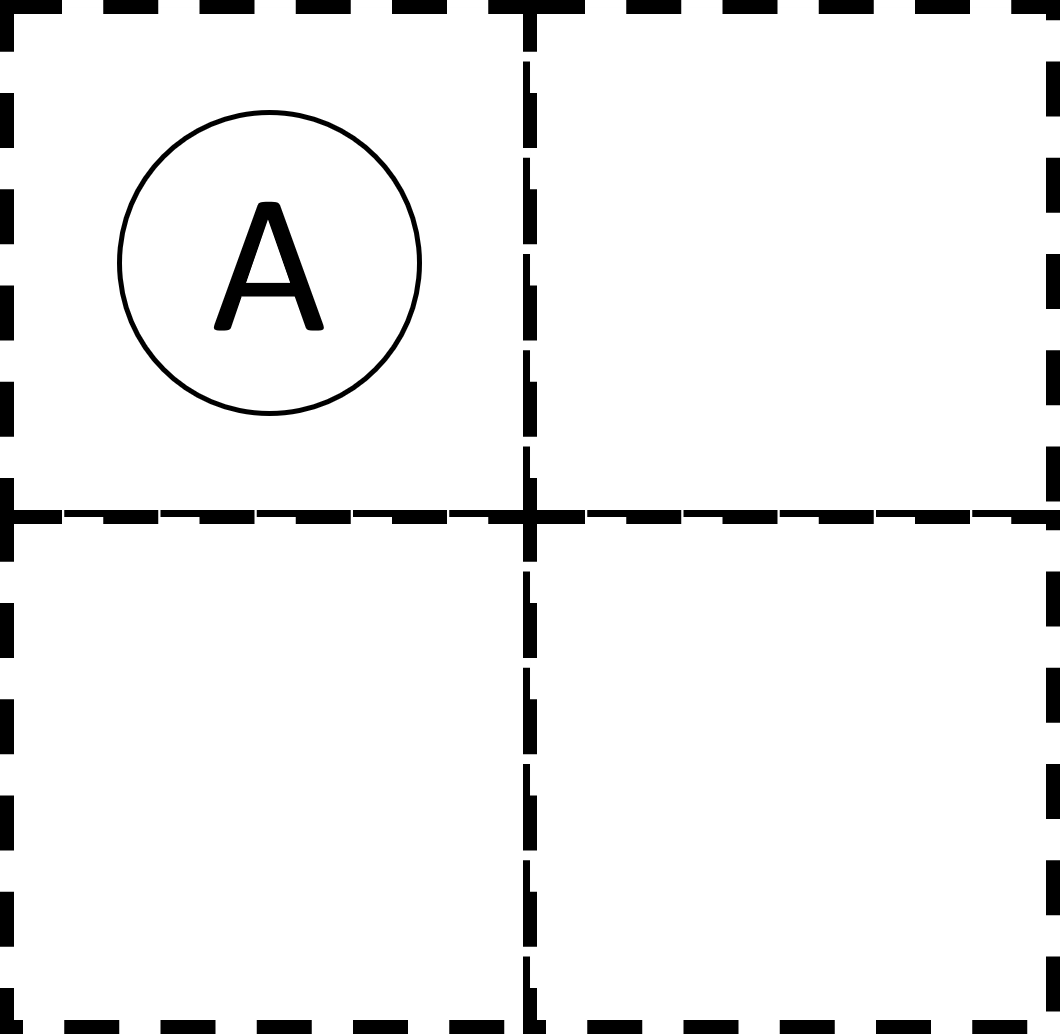
\includegraphics[width=0.5\linewidth]{2MathematicalFramework/Images/2x2_no_walls_world_states/w0.png}
		\caption{$w_{0}$}
		\vspace{0.25cm}
	\end{subfigure}
	\begin{subfigure}[b]{0.45\linewidth}
		\centering
		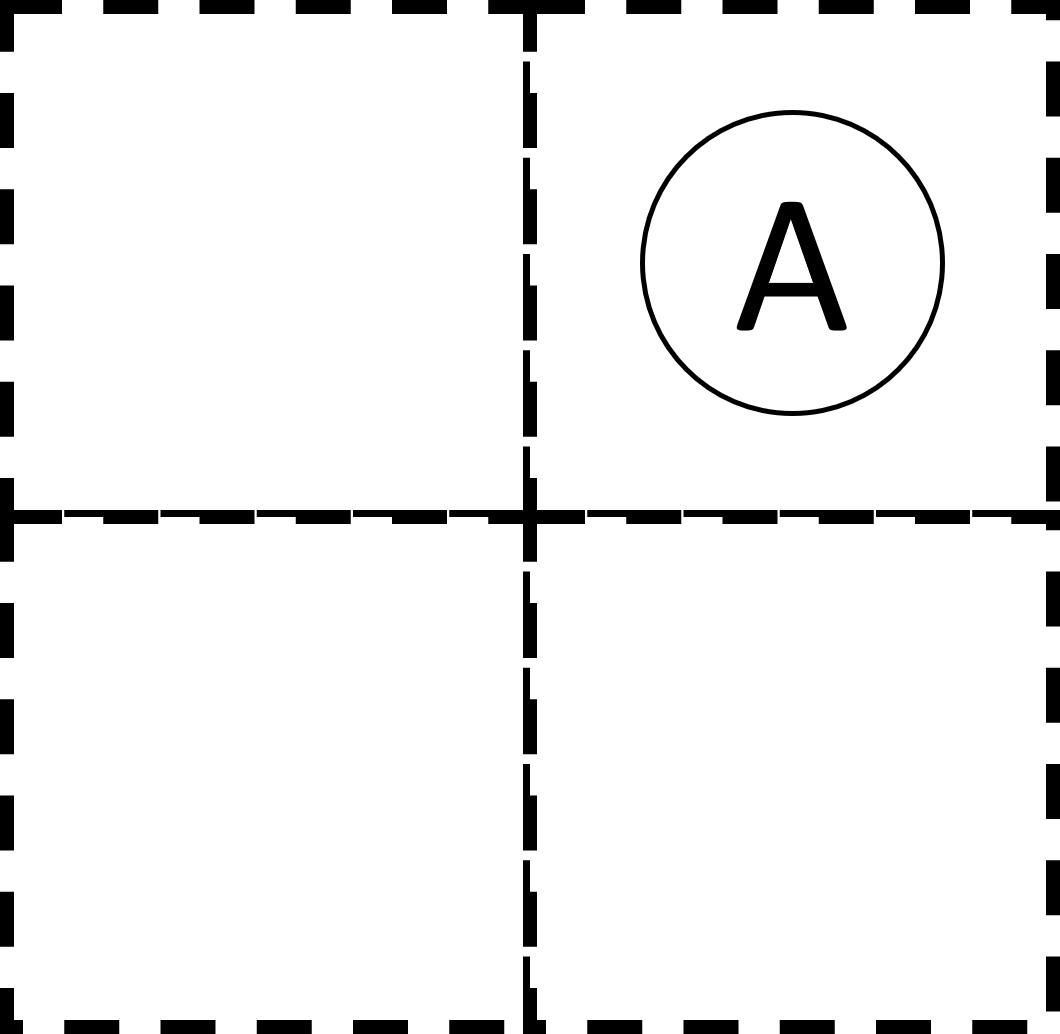
\includegraphics[width=0.5\linewidth]{2MathematicalFramework/Images/2x2_no_walls_world_states/w1.png}
		\caption{$w_{1}$}
		\vspace{0.25cm}
	\end{subfigure}
	\begin{subfigure}[b]{0.45\linewidth}
		\centering
		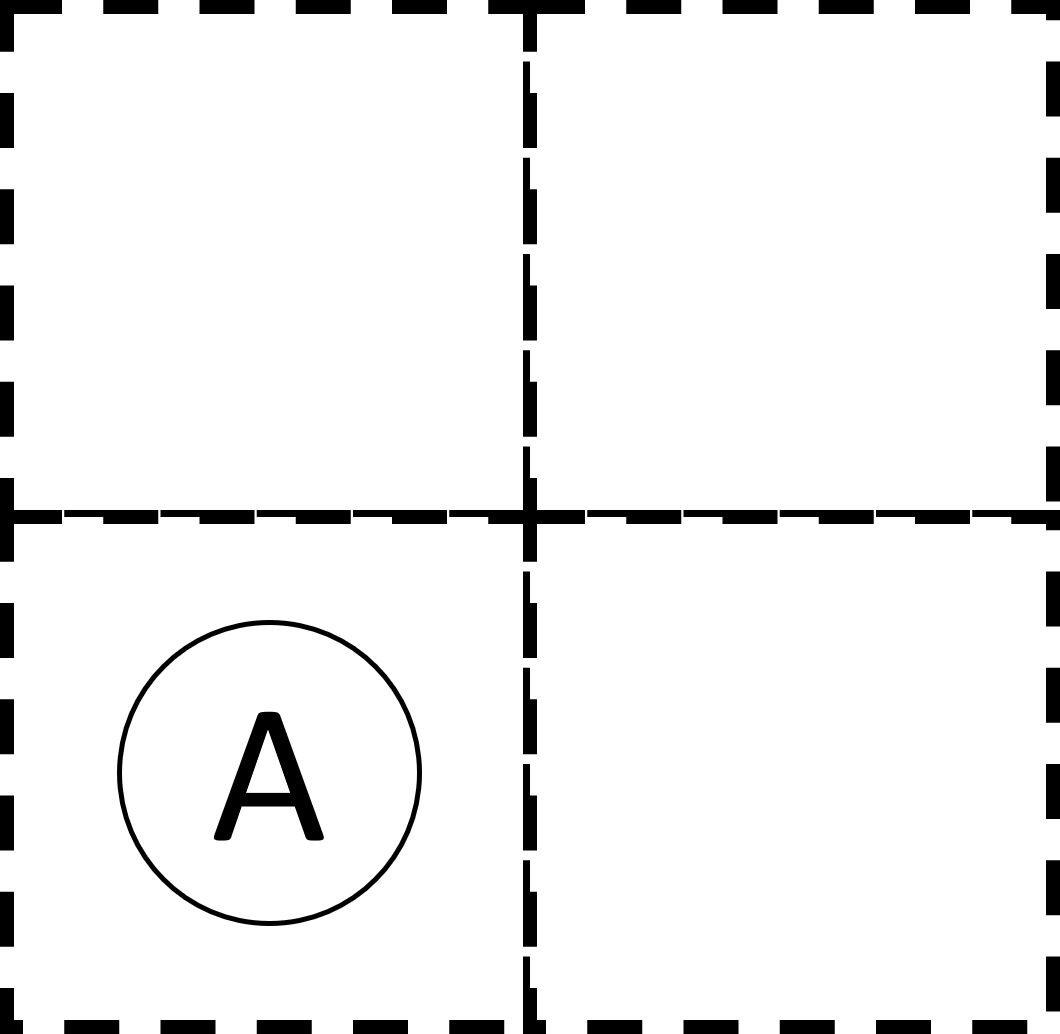
\includegraphics[width=0.5\linewidth]{2MathematicalFramework/Images/2x2_no_walls_world_states/w2.png}
		\caption{$w_{2}$}
	\end{subfigure}
	\begin{subfigure}[b]{0.45\linewidth}
		\centering
		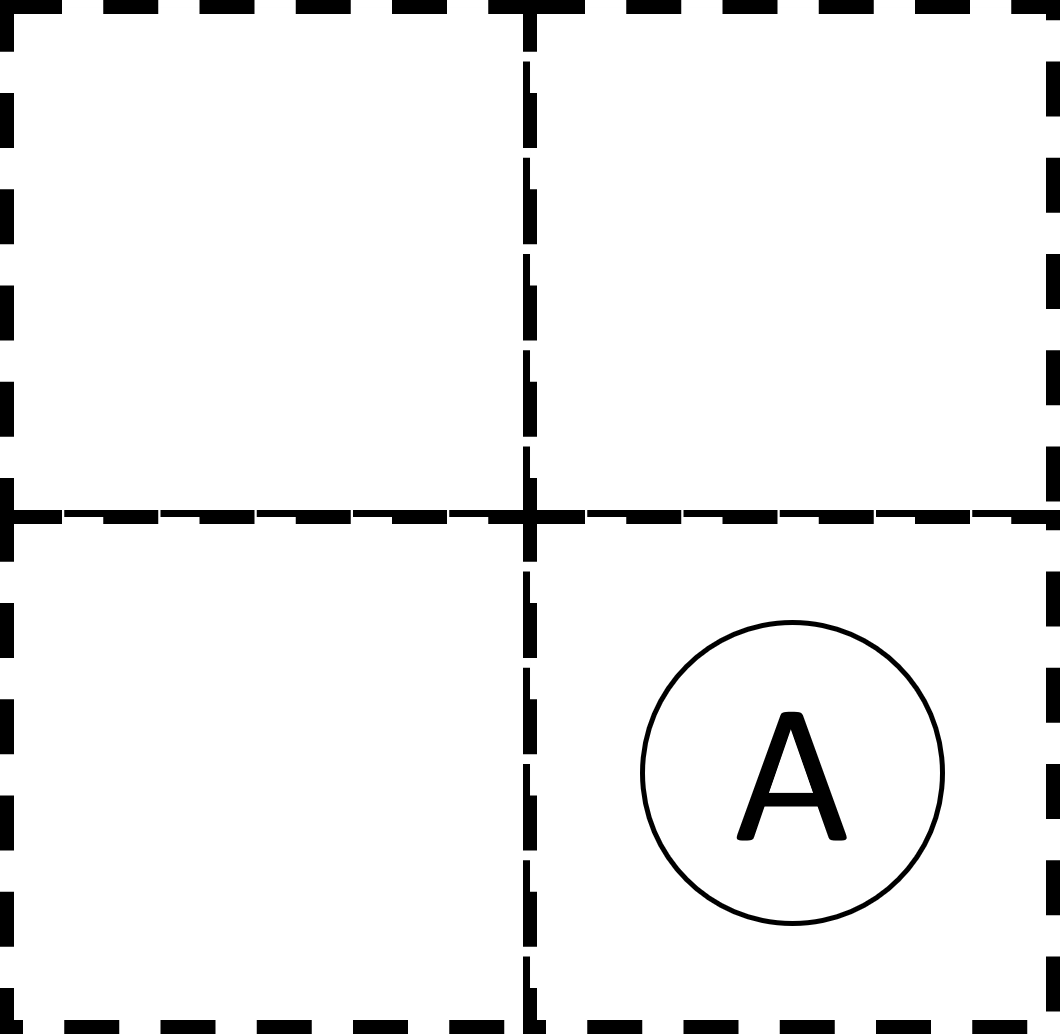
\includegraphics[width=0.5\linewidth]{2MathematicalFramework/Images/2x2_no_walls_world_states/w3.png}
		\caption{$w_{3}$}
	\end{subfigure}
	\caption{
		The world states of a cyclical $2\times 2$ grid world $W_{(2,2)C}$.
		The position of the agent in the world is represented by the position of the circled A.
		\draftnote{blue}{awjdean}{Include a compass in the figure?}
	}
	\label{fig:2x2-cyclical-grid-world-states}
\end{figure}

%%%%%%%%%%%%%%%%%%%%%%%%%%%%%%%%%%%%%%%%%%%%%%%%%%%%%%%%%%%%%%%%%%%%%%%%%%%%%%%%%%%%%%%%%%%%%%
\subsection{Transformations of $\mathscr{W}_{\alpha}$}

We define that there are 24 atomic transformations in $\mathscr{W}_{\alpha}$: the 20 transformations of length 1 given in \cref{tab:2x2_gridworld_length_1_transformations}\footnote{
	We have chosen these because we know the actions we will give the agent in \cref{sec:Actions of the agent in example}; there is a link between the structure of a world from the agent's perspective and the actions the agent will perform - more on this later.
	However, these are the only transformations that are possible for a world with the world states given in \cref{sec:World states of example}, the condition that all the transformations of the world are due to the actions of an agent with the actions provided in \cref{sec:Actions of the agent in example}, and obeying action condition \cref{actcon:action_gives_single_outcome}.
	\draftnote{blue}{awjdean}{Put proof of this in appendices ?}
}
and the 4 trivial transformations $1_{w_{0}}$, $1_{w_{1}}$, $1_{w_{2}}$, and $1_{w_{3}}$.
So for $\mathscr{W}_{\alpha}$, $D_{\varepsilon} = \{ 1_{w_{0}}, 1_{w_{1}}, 1_{w_{3}}, 1_{w_{4}} \}$ and $\hat{D} = \{ d_{1}, d_{2}, d_{3}, \dots, d_{20} \} \cup D_{\varepsilon}$.

\begin{table}[H]
	\centering
	\begin{tabular}{|c|c c|}
		\hline
		Element of $\hat{D} \backslash D_{\varepsilon}$ & Source  & Target  \\
		\hline
		$d_{1}$                                      & $w_{0}$ & $w_{0}$ \\
		$d_{2}$                                      & $w_{0}$ & $w_{1}$ \\
		$d_{3}$                                      & $w_{0}$ & $w_{1}$ \\
		$d_{4}$                                      & $w_{0}$ & $w_{2}$ \\
		$d_{5}$                                      & $w_{0}$ & $w_{2}$ \\
		$d_{6}$                                      & $w_{1}$ & $w_{1}$ \\
		$d_{7}$                                      & $w_{1}$ & $w_{0}$ \\
		$d_{8}$                                      & $w_{1}$ & $w_{0}$ \\
		$d_{9}$                                      & $w_{1}$ & $w_{3}$ \\
		$d_{10}$                                     & $w_{1}$ & $w_{3}$ \\
		$d_{11}$                                     & $w_{2}$ & $w_{2}$ \\
		$d_{12}$                                     & $w_{2}$ & $w_{0}$ \\
		$d_{13}$                                     & $w_{2}$ & $w_{0}$ \\
		$d_{14}$                                     & $w_{2}$ & $w_{3}$ \\
		$d_{15}$                                     & $w_{2}$ & $w_{3}$ \\
		$d_{16}$                                     & $w_{3}$ & $w_{3}$ \\
		$d_{17}$                                     & $w_{3}$ & $w_{1}$ \\
		$d_{18}$                                     & $w_{3}$ & $w_{1}$ \\
		$d_{19}$                                     & $w_{3}$ & $w_{2}$ \\
		$d_{20}$                                     & $w_{3}$ & $w_{2}$ \\
		\hline
	\end{tabular}
	\caption{The transformations of length 1 in $\mathscr{W}_{\alpha}$.}
	\label{tab:2x2_gridworld_length_1_transformations}
\end{table}

It's useful to look at the world diagram\footnote{
We have deliberately positioned the vertices of our world diagram where we have to mirror the structure we perceive it to have (e.g., the line from the $w_{0}-w_{1}$ plane is perpendicular to the $w_{0}$-$w_{2}$ plane); however many valid (isomorphic) world diagrams do not have this feature.
For example:
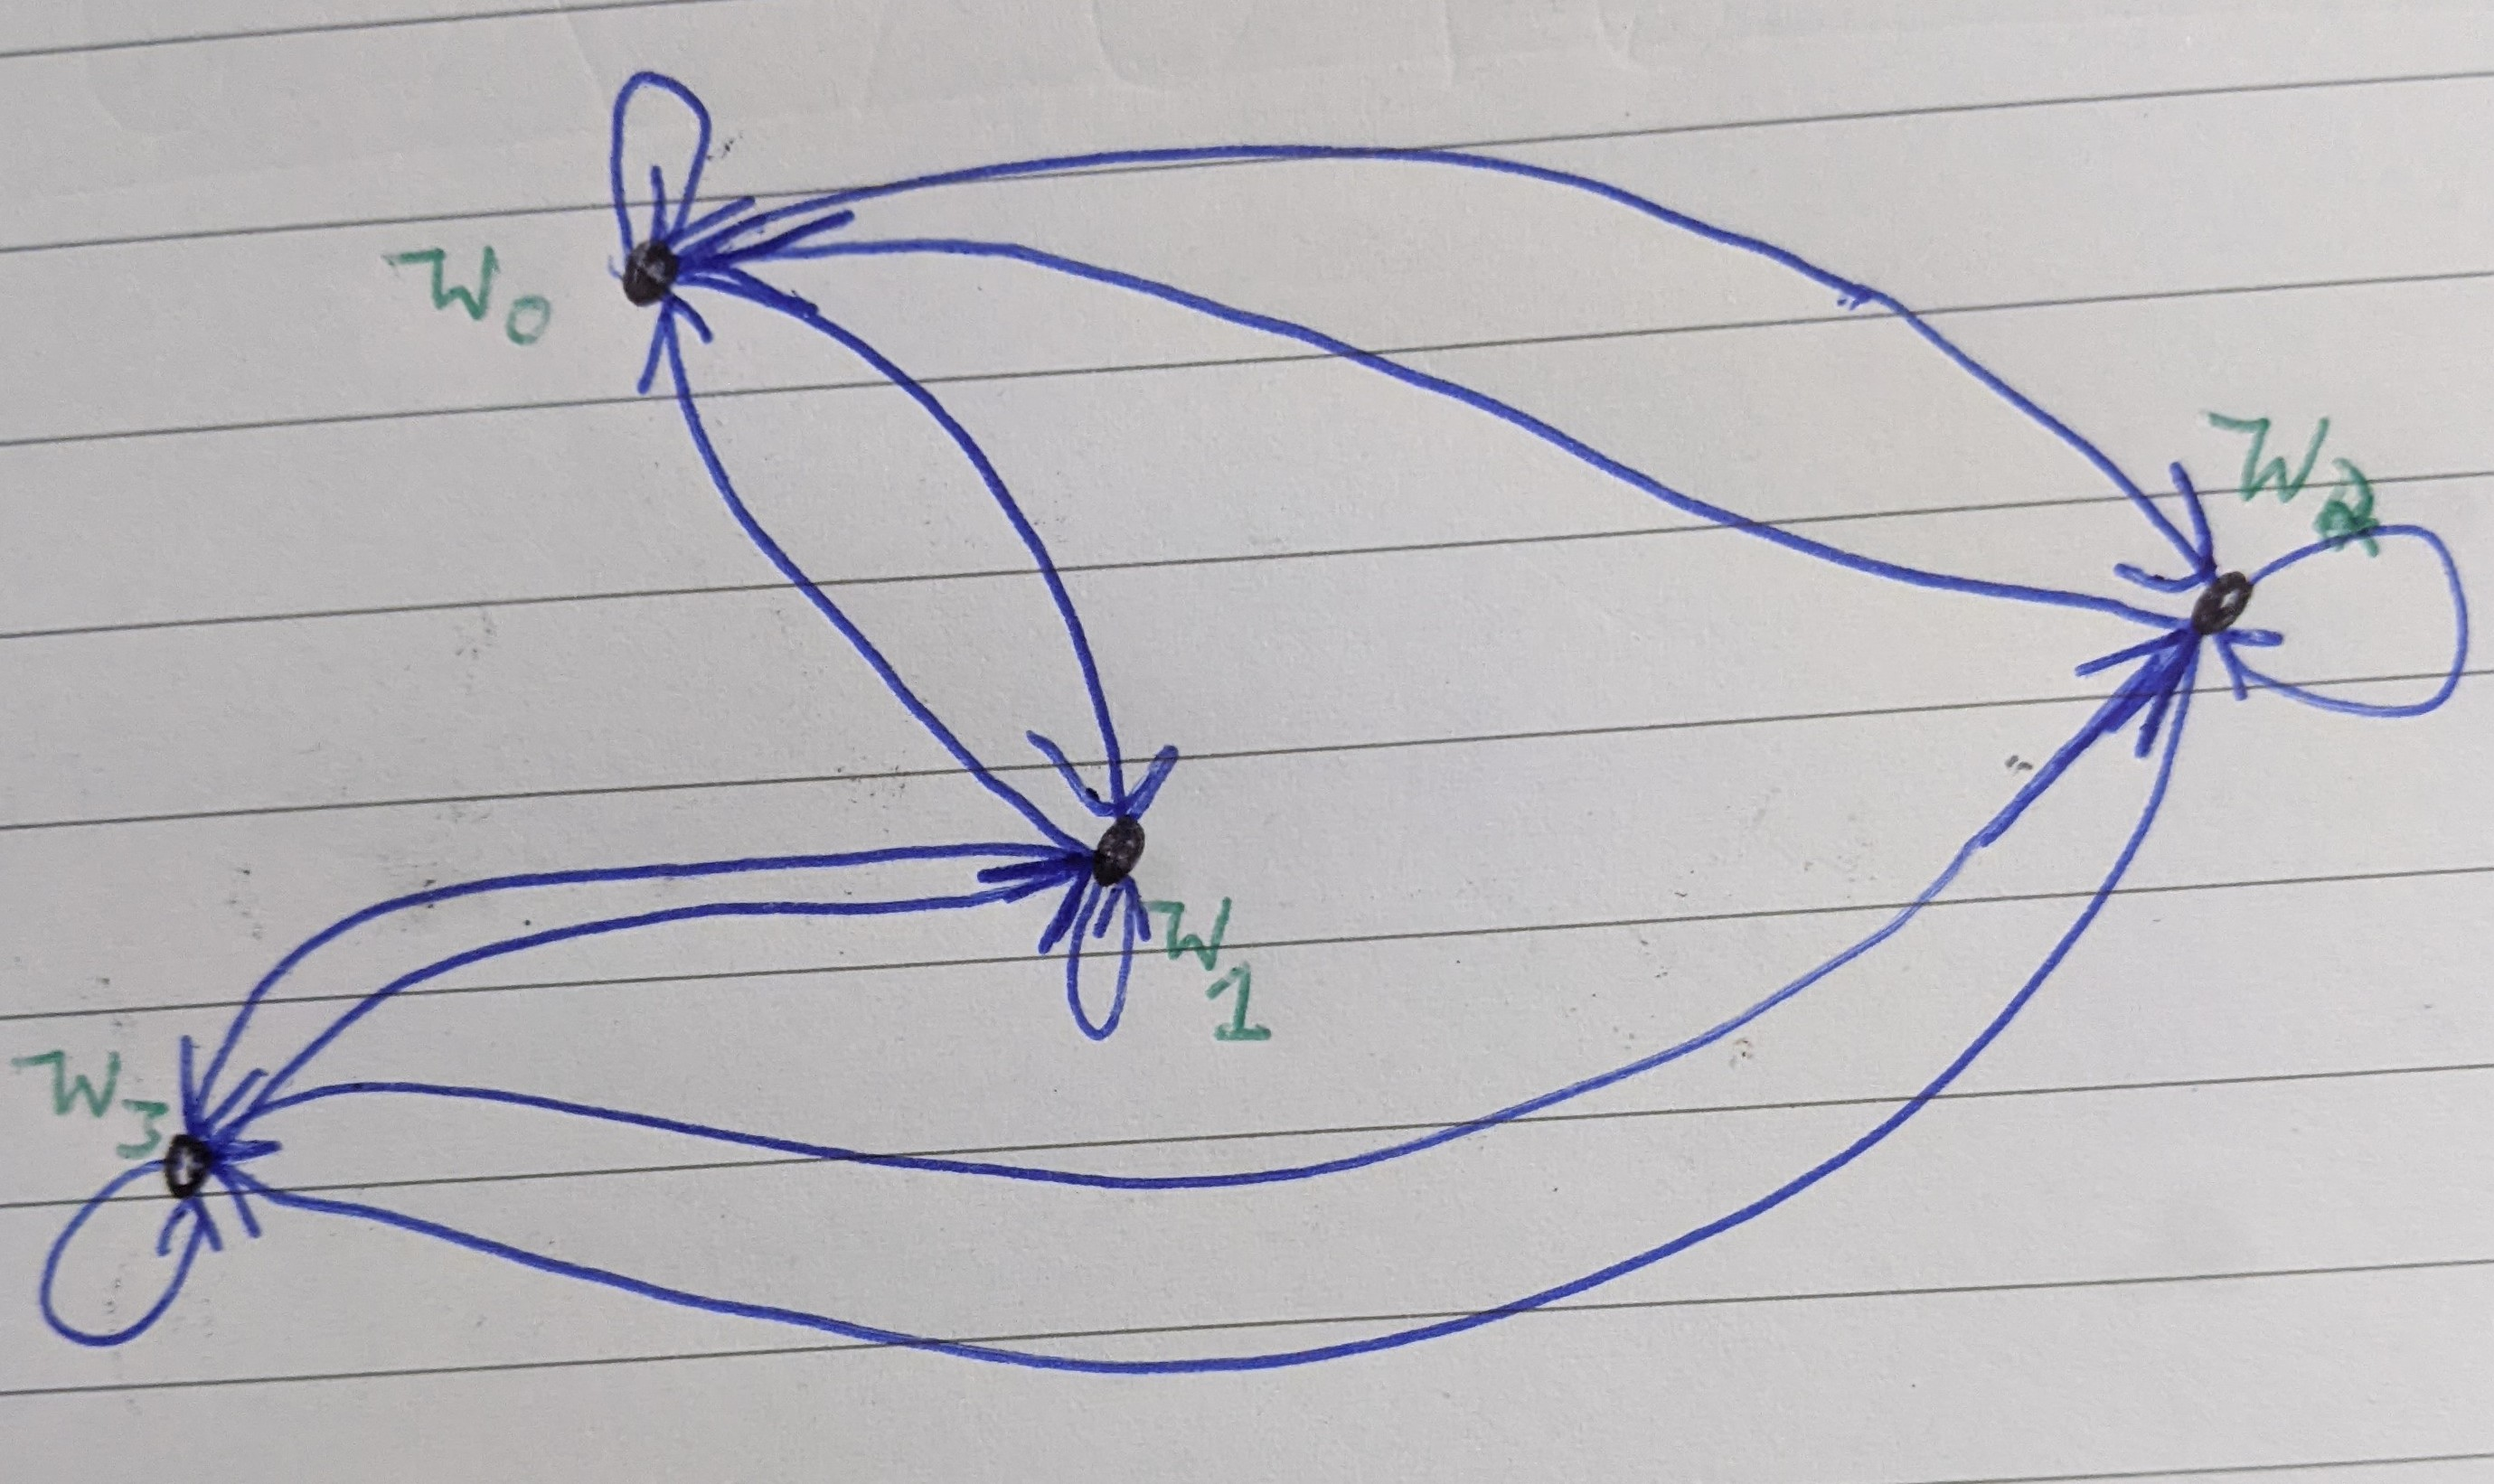
\includegraphics[width=0.5\linewidth]{2MathematicalFramework/Images/2x2_cyclical_min_trans_quirky.jpg}
}
containing the world states and the atomic transformations given in \cref{fig:2x2_cyclical_minimum_transformations}, since this displays the transformation structure of $\mathscr{W}_{\alpha}$ in a more intuitive way than giving the definitions of each atomic transformation as shown in $D_{\varepsilon}$ and \cref{tab:2x2_gridworld_length_1_transformations}.

\begin{figure}[H]
	\centering
	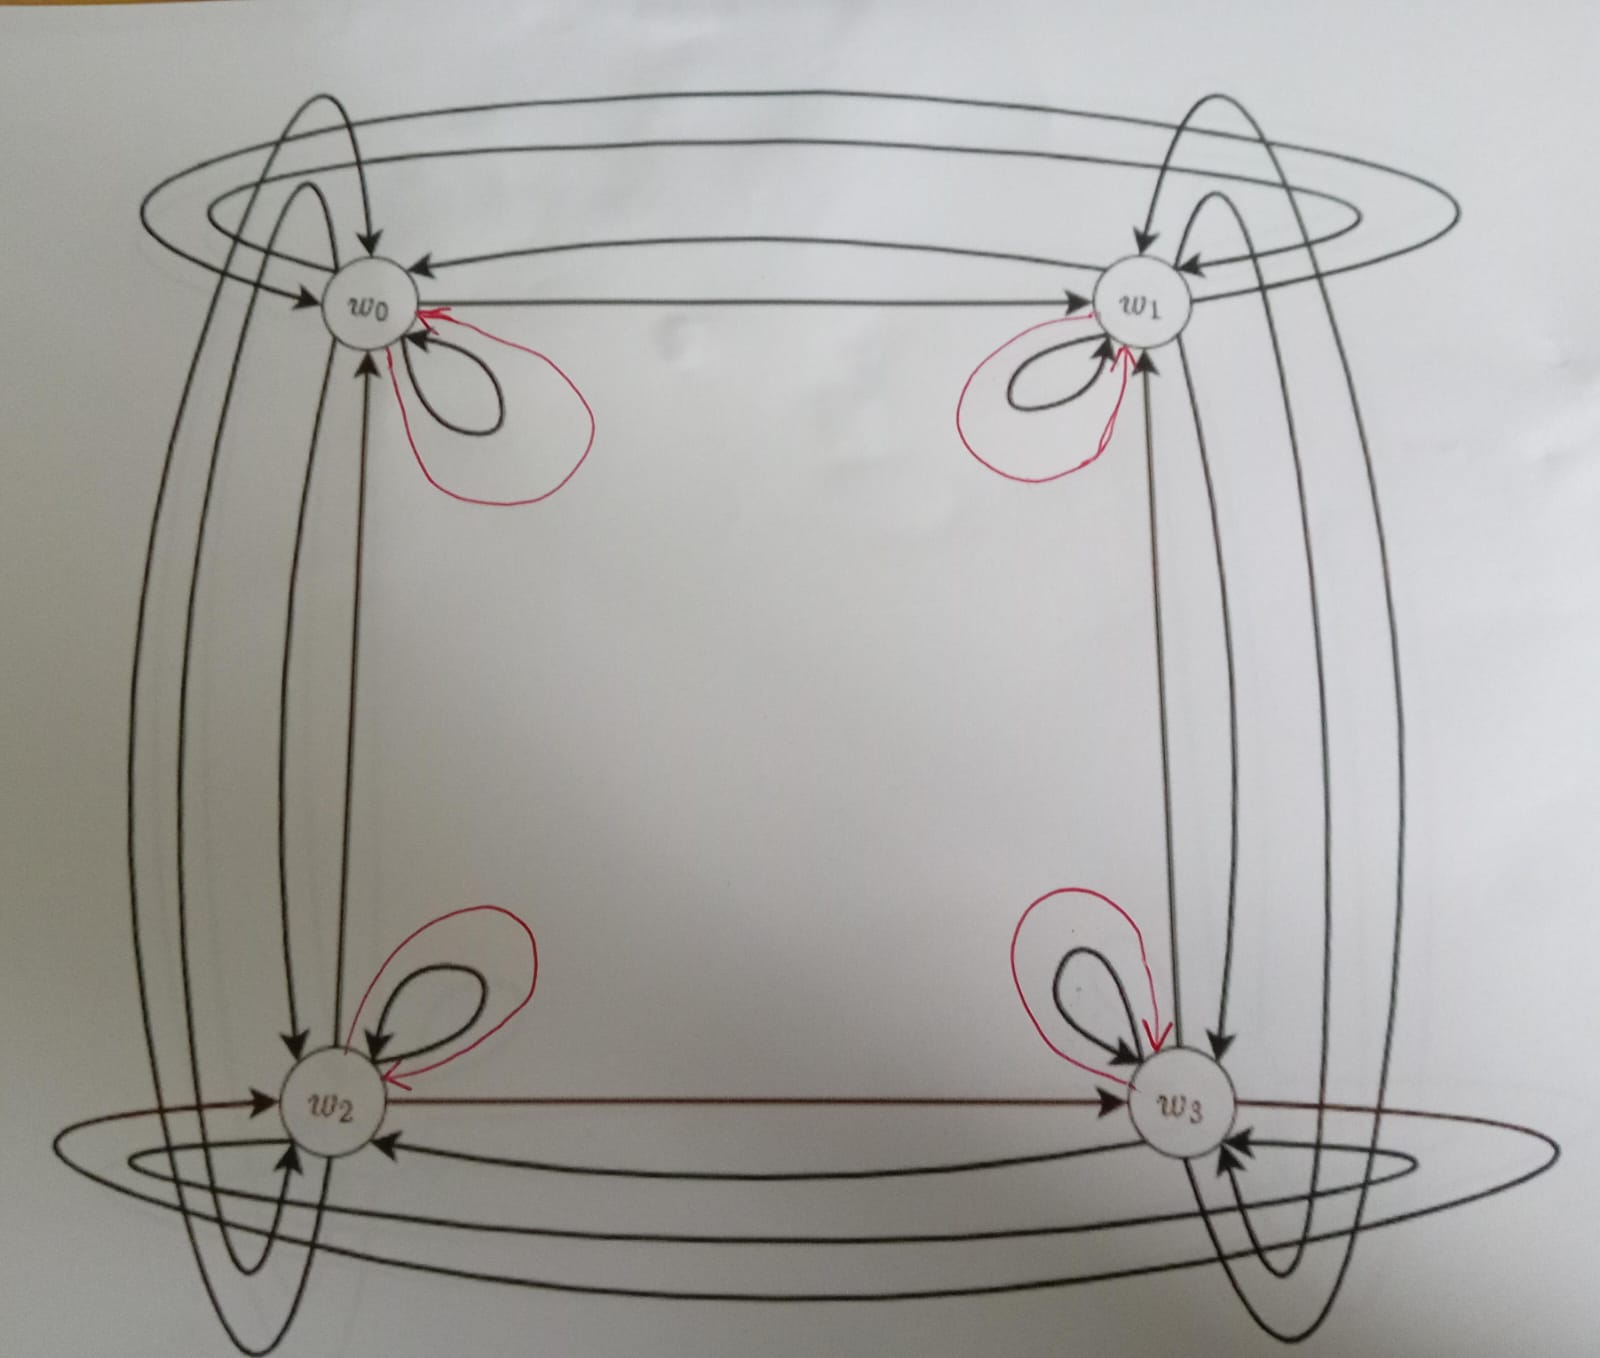
\includegraphics[width=0.5\linewidth]{2MathematicalFramework/Images/2x2_cyclical_minimum_transformations.jpeg}
	\caption{
		A world diagram of $\mathscr{W}_{\alpha}$ containing the transformations in $\hat{D}$.
		Transformations in $D_{\varepsilon}$ are in red.
	}
	\label{fig:2x2_cyclical_minimum_transformations}
\end{figure}

\draftnote{blue}{awjdean}{Something about the structure of $D$ ?}

%%%%%%%%%%%%%%%%%%%%%%%%%%%%%%%%%%%%%%%%%%%%%%%%%%%%%%%%%%%%%%%%%%%%%%%%%%%%%%%%%%%%%%%%%%%%%%
\subsection{Introducing the agent}

We consider an agent with ideal sensors.
This means there is a one-to-one correspondence between world states visited by the agent and the agent's observations.
Since there are 4 world states, the agent has 4 possible observation states $O = \{ o_{0}, o_{1}, o_{2}, o_{3} \}$ where $b(w_{i}) = o_{i}$ for $i = \{0, 1, 2, 3 \}$.
The agent also has, once it has fully learned the structure of $\mathscr{W}_{\alpha}$, four representation states $Z = \{ z_{0}, z_{1}, z_{2}, z_{3} \}$ where $h(o_{i}) = z_{i}$ for $i = \{0, 1, 2, 3 \}$.
Therefore, we have a bijective map $f = hb$ where $f(w_{i}) = z_{i}$ for $i = \{0, 1, 2, 3 \}$.

\draftnote{blue}{awjdean}{Talk about states not visited by the agent here ?}

%%%%%%%%%%%%%%%%%%%%%%%%%%%%%%%%%%%%%%%%%%%%%%%%%%%%%%%%%%%%%%%%%%%%%%%%%%%%%%%%%%%%%%%%%%%%%%
\subsection{
	Actions of the agent in $\mathscr{W}_{\alpha}$
}\label{sec:Actions of the agent in example}

Our agent has the following minimum actions: $\hat{A} = \{ 1, U, D, L, R \}$ as shown in \cref{tab:actions_of_agent_2_by_2_cyclical}.
\begin{table}[H]
	\centering
	\begin{tabular}{|c|c|}
		\hline
		Action                    & Element of $\hat{A}$ \\
		\hline
		Move up                   & $U$                  \\
		\hline
		Move down                 & $D$                  \\
		\hline
		Move right                & $R$                  \\
		\hline
		Move left                 & $L$                  \\
		\hline
		Do nothing (no op action) & $1$                  \\
		\hline
	\end{tabular}
	\caption{Minimum actions of agent in $\mathscr{W}_{\alpha}$.}
	\label{tab:actions_of_agent_2_by_2_cyclical}
\end{table}

Earlier we described the world $\mathscr{W}_{\alpha}$ as \emph{cyclical}.
Now we are dealing with actions in our toy example, we can finally state what we mean by a cyclical world.
A world $\mathscr{W} = $ is \emph{cyclical} if for any $a \in A$ and $w \in W$, there exists a positive integer $n \in \mathbb{N}^{+}$ such that $a^{n} \ast w = w$; in other words, a world is cyclical if the world returns to its starting state when any action is performed enough times\footnote{
	If the world returns to its starting state when only certain actions are applied enough times, then we say the world is \emph{cyclical with respect to those actions}.
	Sometimes, cyclical structure might be present for a certain actions (e.g., $a_{1}$, $a_{2}$) starting from certain world states (e.g., $w$, $w'$), but not starting from other world states; in these cases we can say the world is cyclic with respect to $(a_{1}, a_{2}; w, w')$.
}.
For our example world $\mathscr{W}_{\alpha}$, informally, this means that if the embodied agent goes through the top(/bottom/right/left) of side of the world then it will reappear at the bottom(/top/left/right) side.
This behaviour is similar to that found in games like Pac-Man \draftnote{blue}{awjdean}{Reference} or Snake \draftnote{blue}{awjdean}{Reference}.
A more precise example would be that if the embodied agent performs the up action while $\mathscr{W}_{\alpha}$ is in world state $w_{0}$ then $\mathscr{W}_{\alpha}$ will transform into world state $w_{2}$.

Before we label the transformations in $D$ with their associated actions, we must identify which transformations should be labelled and how (i.e, we must identify the elements of the sets $\hat{D}_{A}$ and $D_{A}$).
For our example world $\mathscr{W}_{\alpha}$, the procedure outlined in \cref{fig:action_labelling_procedure} in somewhat simplified because all the transformations in $\mathscr{W}_{\alpha}$ are due to the actions of the agent embodied in the world; this means that $\hat{D} = \hat{D}_{A}$\footnote{so $\hat{D}_{A} = \{ d_{1}, d_{2}, d_{3}, \dots, d_{20} \} \cup D_{\varepsilon}$.}, and therefore $\mathscr{W} = \mathscr{W}_{A}$ and $D = D_{A}$.

The transformations of $\mathscr{W}_{\alpha}$ due to the agent's minimum actions (i.e., the effect of the minimum actions on the world states $W$) are shown in \cref{tab:2x2_gridworld_minimum_actions}.
Since all transformations of $\mathscr{W}_{\alpha}$ are due to the actions of the agent, this table shows all the atomic transformations in $\mathscr{W}_{\alpha}$ and how they are labelled using the labelling map $l$.

\begin{table}[H]
	\centering
	\begin{tabular}{c c}
		                    & Minimum action                                                                                                                                                                                                        \\
		Initial world state & \begin{tabular}{c|c c c c c}
			                              & $1$     & $U$     & $D$     & $L$     & $R$     \\
			                      \hline
			                      $w_{0}$ & $w_{0}$ & $w_{2}$ & $w_{2}$ & $w_{1}$ & $w_{1}$ \\
			                      $w_{1}$ & $w_{1}$ & $w_{3}$ & $w_{3}$ & $w_{0}$ & $w_{0}$ \\
			                      $w_{2}$ & $w_{2}$ & $w_{0}$ & $w_{0}$ & $w_{3}$ & $w_{3}$ \\
			                      $w_{3}$ & $w_{3}$ & $w_{1}$ & $w_{1}$ & $w_{2}$ & $w_{2}$ \\
		                      \end{tabular} \\
	\end{tabular}
	\caption{
		Each entry in this table shows the outcome state of the agent performing the action given in the column label when in the world state given by the row label.
		\draftnote{blue}{awjdean}{Improve this caption - talk about the action effect operator ($\ast$).
			Fix centering of "Minimum action" and "Initial world state".}
	}
	\label{tab:2x2_gridworld_minimum_actions}
\end{table}

We can use \cref{tab:2x2_gridworld_minimum_actions} to construct the labelling map $\hat{l}$ - the construction of $\hat{l}$ and $l$ and the generation of \cref{tab:2x2_gridworld_minimum_actions} would happen during the agent's learning process.

\begin{table}[H]
	\centering
	\begin{tabular}{|c|cc||c|}
		\hline
		$d \in \hat{D}$ & $s(d)$  & $t(d)$  & $\hat{l}(d)$ \\
		\hline
		$d_{1}$         & $w_{0}$ & $w_{0}$ & $1$          \\
		$d_{2}$         & $w_{0}$ & $w_{1}$ & $R$          \\
		$d_{3}$         & $w_{0}$ & $w_{1}$ & $L$          \\
		$d_{4}$         & $w_{0}$ & $w_{2}$ & $D$          \\
		$d_{5}$         & $w_{0}$ & $w_{2}$ & $U$          \\
		$d_{6}$         & $w_{1}$ & $w_{1}$ & $1$          \\
		$d_{7}$         & $w_{1}$ & $w_{0}$ & $L$          \\
		$d_{8}$         & $w_{1}$ & $w_{0}$ & $R$          \\
		$d_{9}$         & $w_{1}$ & $w_{3}$ & $D$          \\
		$d_{10}$        & $w_{1}$ & $w_{3}$ & $U$          \\
		$d_{11}$        & $w_{2}$ & $w_{2}$ & $1$          \\
		$d_{12}$        & $w_{2}$ & $w_{0}$ & $U$          \\
		$d_{13}$        & $w_{2}$ & $w_{0}$ & $D$          \\
		$d_{14}$        & $w_{2}$ & $w_{3}$ & $R$          \\
		$d_{15}$        & $w_{2}$ & $w_{3}$ & $L$          \\
		$d_{16}$        & $w_{3}$ & $w_{3}$ & $1$          \\
		$d_{17}$        & $w_{3}$ & $w_{1}$ & $U$          \\
		$d_{18}$        & $w_{3}$ & $w_{1}$ & $D$          \\
		$d_{19}$        & $w_{3}$ & $w_{2}$ & $L$          \\
		$d_{20}$        & $w_{3}$ & $w_{2}$ & $R$          \\
		$1_{w_{0}}$     & $w_{0}$ & $w_{0}$ & $\varepsilon$   \\
		$1_{w_{1}}$     & $w_{1}$ & $w_{1}$ & $\varepsilon$   \\
		$1_{w_{2}}$     & $w_{2}$ & $w_{2}$ & $\varepsilon$   \\
		$1_{w_{3}}$     & $w_{3}$ & $w_{3}$ & $\varepsilon$   \\
		\hline
	\end{tabular}
	\caption{
		Labelling map $\hat{l}$ for $\mathscr{W}_{\alpha}$.
	}
	\label{tab:2x2_cyclical_labelling_with_min_actions}
\end{table}

The application of the labelling map $\hat{l}$ as a world diagram is shown in \cref{fig:2x2_cyclical_labelling_with_min_actions}\footnote{
	It's important to note that the no-op action $1$, where the agent does nothing, does not label the trivial transformations $1_{w}$, which are labelled by the empty action $\varepsilon$.
	This means the no-op action does not act as an identity element for $(\hat{A}\ast, \circ)$.
}.

\begin{figure}[H]
	\centering
	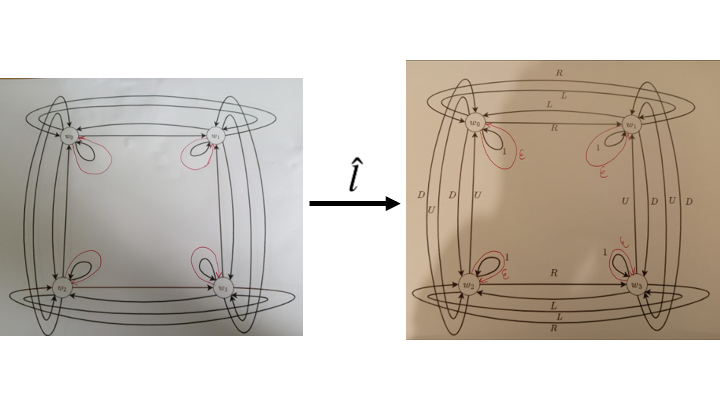
\includegraphics[width=1\linewidth]{2MathematicalFramework/Images/2x2_cyclical_labelling_with_min_actions.png}
	\caption{
		World diagram for $\mathscr{W}_{\alpha}$ showing how $\hat{l}$ labels the minimum action transformations.
	}
	\label{fig:2x2_cyclical_labelling_with_min_actions}
\end{figure}

Remember, \cref{fig:2x2_cyclical_labelling_with_min_actions} only shows the minimum action transformations in $\hat{D}_{A}$ labelled by there associated minimum actions in $\hat{D}$ - we only show these transformations for simplicity.

When considering the full transformation structure of $\mathscr{W}_{\alpha}$, there will be transformations between any two world states; for example, $d_{9} \circ d_{1}: w_{0} \to w_{3}$.
In fact, there are a (countably) infinite number of transformations in $D$ between any two world states; for example, $D \circ R$, $D \circ R \circ 1^{n}$ ($n \in \mathbb{N}$), $1^{n} \circ D \circ R$ ($n \in \mathbb{N}$), $D \circ R \circ (L \circ R)^{n}$ ($n \in \mathbb{N}$) etc...
Similarly, there are a (countably) infinite number of actions in $A$ between any two world states\footnote{Although the set $A$ is less dense or as dense as $D$. \draftnote{blue}{awjdean}{Explore this further in appendices.}} - just take the actions in $A$ that labels each of the transformations in $D$ we just described.

%%%%%%%%%%%%%%%%%%%%%%%%%%%%%%%%%%%%%%%%%%%%%%%%%%%%%%%%%%%%%%%%%%%%%%%%%%%%%%%%%%%%%%%%%%%%%%
\draftnote{green}{To do}{
	\begin{enumerate}
		\item Show parts of: $\hat{A}^{\ast}$, $D$
		\item Summary at end: State what each of the things are shown in \cref{fig:action_labelling_procedure}.
		\item In section introduction --> say toy example inspired by Higgins (2018) + Caselles Dupres (?)
		\item Show example of atomic transformations in $\hat{D}_{A}$ - example with intermediate world states that are skipped over by transformations due to actions of agent.
		\item Change symbol for $\mathscr{W}_{\alpha}$ to include agent ? -- add agent to $(W, \hat{D}. s, t)$ ?
		\item Label the transformation diagrams with their symbols ($d_{1}$, $d_{2}$ etc...) ?
		\item Switch $U$, $D$, $R$, $L$ into $N$, $S$, $E$, $W$ --> makes sense when giving agent ability to rotate. What to do about $W$ also being the symbol for the set of world states ?
		      \begin{compactitem}
			      \item When doing the 'rotate 90 degrees and move forwards" agent, need to talk about how we usually only consider the transinformation of the world (arrows) for our specific agent, but in reality there are all possible transformations ? (otherwise $D$ looks different for agents with different actions - is that necessarily a bad thing or is it what we want ?)
		      \end{compactitem}
		\item \textbf{Appendices:} Size of $D$ and $A$: $D$ and $A$ countably infinite, $A$ more sparse than $D$.
		      \begin{compactitem}
			      \item Proof that $D$ and $A$ are countably infinite.
			      \item \textbf{Mention:} We only consider finite walks because we were worried that including infinite walks would complicate the work; how including infinite walks would affect things is a potential direction for future study. Out guess is that including infinite walks should not affect things.
			      \item Consider "Directed Walks $\&$ density of A vs D".
			      \item Asymptotic density of A vs D --> for $\mathscr{W}_{\alpha}$, I think it might be $\rho_{D}(A) = \frac{1}{5}$ because there are 4 elements in $\hat{A}$.
		      \end{compactitem}
		\item Example.
		      \begin{compactitem}
			      \item Diagram (l-map-for-transformations-from-and-to-w0).
			      \begin{compactitem}
				      \item This diagram shows how the atomic transformations $d$ with $d(s) = w_{0}$ or $d(t)= w_{0}$ are mapped to actions using the map $l$.
				      \item Figure ref[fig:l-map-for-transformations-from-and-to-w0] demonstrates how the map $l$ maps transformations in $D$ to the elements in $A$ for the transformations shown in Figure ref[fig:2x2-cyclical-min-actions-standard].
			      \end{compactitem}
		      \end{compactitem}
	\end{enumerate}
}

\draftnote{blue}{Questions/thoughts that have been answered}{
	\begin{enumerate}
		\item Are the elements $1_{w}$ in $\hat{D}$ ? At the moment - yes.
		      \begin{compactitem}
			      \item \textbf{Counter:} Making $\hat{D}$ not include $D_{\varepsilon}$ would line the notation up with $\hat{A}$.
		      \end{compactitem}
	\end{enumerate}
}

%%%%%%%%%%%%%%%%%%%%%%%%%%%%%%%%%%%%%%%%%%%%%%%%%%%%%%%%%

%%%%%%%%%%%%%%%%%%%%%%%%%%%%%%%%%%%%%%%%%%%%%%%%%%%%%%%%%
\section{Structure through equivalence}
%%%%%%%%%%%%%%%%%%%%%%%%%%%%%%%%%%%%%%%%%%%%%%%%%%%%%%%%%
\subsection{Motivation}

\draftnote{blue}{Include}{
Something about how extracting the global algebra provides potential for generalisation compared to learning each individual labelled transformation.
}

\newthought{Consider a world-agent} pair $\mathscr{W}$-$\mathscr{A}$.
Our algebra of actions $(\hat{A}^{*}, \circ)$ is a free monoid, which is the same for any world.
This free monoid $\hat{A}^{*}$ is the most general, and therefore the most structure free, monoid constructed from the atomic actions in $\hat{A}$ - its structure only depends on the atomic actions in $\hat{A}$\footnote{
In fact, any monoid generated by $\hat{A}$ can be obtained by imposing additional structure, in the form of relations, on $\hat{A}^{*}$, and so every monoid can be viewed as a quotient of $\hat{A}^{*}$ under some relation.
}.
However, we expect that there must be more structure we can tease out of our $(\hat{A}^{*}, \circ)$ since it appears that different worlds have different transformation structures.

Now remember the transformation structure of the world due to the actions of an agent is captured by the monoid action $(\hat{A}^{*}, \circ, \ast)$.
It would be useful if we could abstract how actions behave in the world from the individual world states by extracting aspects of the transformation structure of the world $\mathscr{W}$ into the monoid $(\hat{A}^{*}, \circ)$ through a relation.
Additionally, if we want to find other recognisable algebraic structures (e.g., groups, semigroups etc...) in the structure of worlds, we need a way of saying collections of transformations (i.e., the actions that are elements of $\hat{A}^{*}$) are the same in some way, otherwise, there is no way to satisfy the requirements of these algebras\footnote{
For example, for the group inverse property to be satisfied we need, for each $a \in \hat{A}^{*}$, an element $a'$ in $\hat{A}^{*}$ such that
\begin{align}
    & a' \circ a = e \\
    & a \circ a' = e.
\end{align}
where $e$ is the identity element.
}.

\newthought{So we want} a relation on the actions in $\hat{A}^{*}$ that (1) gives us a concept of sameness between actions (so we can satisfy requirements of algebraic structures that we want to find), and (2) captures some of the structure of the world in the monoid $(\hat{A}^{*}, \circ)$.
To do this we define an equivalence relation $\sim$ on the elements of $\hat{A}^{*}$; this equivalence relation enforces aspects of the structure of the world onto the free monoid $(\hat{A}^{*}, \circ)$ to give us a new algebra $(\hat{A}^{*}/\sim, \circ_{\sim})$ , where it is now possible to satisfy properties like the inverse condition.
We believe agents can gain a better understanding of the structure of the world though learning the structure of the algebras we will construct using equivalence relations.
In fact, we believe that when an agent is learning the transformation structure of a world, the agent is predominantly learning equivalence relations on $\hat{A}^{*}$ that reflect the transformation structure of the world.


%%%%%%%%%%%%%%%%%%%%%%%%%%%%%%%%%%%%%%%%%%%%%%%%%%%%%%%%%
\subsection{An equivalence relation $\sim$}

\newthought{We define an} equivalence relation on the elements of $\hat{A}^{*}$ that says two actions are equivalent (our sense of the actions being the same) if the actions lead to the same end world state when performed in any initial world state\footnote{
Our use of equivalence relations was inspired by \cite{caselles2020sensory}'s use of an equivalence relation to equate action sequences that produced the same end observation from an initial state \draftnote{blue}{(we discuss issues with \cite{caselles2020sensory}'s approach in section ???)}{}.
We realised that a global version of a similar equivalence relation is exactly the mathematical interpretation of the equality found in \cite{Higgins2018}.
}.
Formally, we define the equivalence $\sim$ as, for two actions $a, a' \in \hat{A}^{*}$,
\begin{equation}
    a \sim a' \iff a \ast w = a' \ast w \quad \text{ for all $w \in W$}.
\end{equation}


\begin{propositionE}
    $\sim$ is an equivalence relation on $\hat{A}^{*}$.
\end{propositionE}
\begin{proofE}
\begin{enumerate}
    \item \textbf{Reflexivity.}
    For any $a \in \hat{A}^{*}$, $a \ast w = a \ast w$ for all $w \in W$ (by reflexivity of equality). Hence $a \sim a$.
    
    \item \textbf{Symmetry.}
    Suppose $a \sim a'$ for $a, a' \in \hat{A}^{*}$.
    \begin{align}
        & a \sim a' \\
        \implies & a \ast w = a' \ast w \quad \text{for all $w \in W$} \\
        \implies & a' \ast w = a \ast w \quad \text{for all $w \in W$} \\
        \implies & a' \sim a
    \end{align}
    
    \item \textbf{Transitivity.}
    Suppose $a \sim a'$ and $a' \sim a''$ for $a, a', a'' \in \hat{A}^{*}$.
    \begin{equation}
        a \sim a' \implies a \ast w = a' \ast w \quad \text{for all $w \in W$}
    \end{equation}
    and
    \begin{equation}
        a' \sim a'' \implies a' \ast w = a'' \ast w \quad \text{for all $w \in W$}.
    \end{equation}
    Therefore,
    \begin{align}
        & a \ast w = a' \ast w \text{ and } a' \ast w = a'' \ast w \quad \text{for all $w \in W$} \\
        \implies & a \ast w = a'' \ast w \quad \text{for all $w \in W$} \\
        \implies & a \sim a''
    \end{align}

    \item \textbf{Conclusion.}
    Since $\sim$ is reflexive, symmetric, and transitive, $\sim$ is an equivalence relation on $\hat{A}^{*}$.
\end{enumerate}
\end{proofE}

\begin{notation}
    We denote the the equivalence class of an action $a \in \hat{A}^{*}$ due to the equivalence relation $\sim$ by  $[a]_{\sim}$.
\end{notation}

We define the canonical projection map $\pi_{\sim}: \hat{A}^{*} \to \hat{A}^{*}/\sim$ that sends actions in $\hat{A}^{*}$ to their equivalence classes $[a]_{\sim}$ under $\sim$ in the quotient set $\hat{A}^{*}/\sim$:
\begin{equation}
\begin{aligned}
    & \pi_{\sim}: \hat{A}^{*} \to \hat{A}^{*}/\sim \quad \text{such that} \\
    & \pi_{\sim}(a) = [a]_{\sim} \quad \text{for all $a \in \hat{A}^{*}$}
\end{aligned}
\end{equation}
where the equivalent classes $[a]_{\sim}$ are the sets
\begin{equation}
	[a]_{\sim} = \{ a' \in \hat{A}^{*} \mid a' \sim a \}
\end{equation}
and the quotient set $\hat{A}^{*}/\sim$ is the collection of all such equivalence classes
\begin{equation}
    \hat{A}^{*}/\sim = \{ [a]_{\sim} \mid a \in \hat{A}^{*} \}.
\end{equation}

We can view the projection map $\pi_{\sim}$ as collapsing actions in $\hat{A}/\sim$ that are indistinguishable in terms of their effect on $W$ into a single representative element in the quotient set $\hat{A}^{*}/\sim$\footnote{
    When we define an equivalence $\sim$ on $\hat{A}^{*}$ to get the set $\hat{A}^{*}/\sim$, we can think of our set $\hat{A}^{*}$ `folding over' on itself to make elements of $\hat{A}^{*}$ that are equivalent stick together.
}.
Since $\sim$ is an equivalence relation, the collection $\hat{A}^{*}/\sim$ of equivalence classes forms a partition of $\hat{A}^{*}$; this means that\footnote{
Formally, $\hat{A}^{*}/\sim$ has the properties of
\begin{enumerate}
    \item \textbf{Coverage.}
    Every action $a \in \hat{A}^{*}$ belongs to some equivalence class $[a]_{\sim}$;

    \item \textbf{Disjointness.}
    For any two actions $a, a' \in \hat{A}^{*}$, either $[a]_{\sim} = [b]_{\sim}$ or $[a]_{\sim} \cap [b]_{\sim} = \emptyset$.
\end{enumerate}
}
\begin{enumerate}
    \item every action in $\hat{A}^{*}$ belongs to an equivalence class in $\hat{A}^{*}/\sim$;
    \item every action in $\hat{A}^{*}$ belongs to exactly one equivalence class in $\hat{A}^{*}/\sim$.
\end{enumerate}

%%%%%%%%%%%%%%%%%%%%%%%%%%%%%%%%%%%%%%%%%%%%%%%%%%%%%%%
\paragraph{Composition of equivalent actions.}
\newthought{We define the} composition operator $\circ_{\sim}$ on the elements in $\hat{A}^{*}/\sim$ using our action composition operator $\circ$ as
\begin{equation}
	\begin{aligned}
		 & \circ_{\sim}: (\hat{A}^{*}/\sim) \times (\hat{A}^{*}/\sim) \to (\hat{A}^{*}/\sim) \quad \text{such that} \\
		 & [a']_{\sim} \circ_{\sim} [a]_{\sim} = [a' \circ a]_{\sim} \quad \text{for $a,a' \in \hat{A}^{*}$}.
	\end{aligned}
\end{equation}

We need to show that the operation $\circ_{\sim}$ on the equivariance classes does not depend on the representative element chosen for those classes; this means we can consistently use any element of an equivalence class as a representative of that class (i.e., the operation $\circ_{\sim}$ is well-defined).

\begin{propositionE}
    \label{prp:circ_sim_well_defined}
    $\circ_{\sim}$ is well-defined on $\hat{A}^{*}/\sim$.
\end{propositionE}
\begin{proofE}
\begin{enumerate}
    \item \textbf{Problem.}
    For $\circ_{\sim}$ to be well-defined on $\hat{A}^{*}/\sim$, we need\footnote{
        \textbf{Well-definedness requirement.}
        An operation on a quotient set
        \begin{equation}
            (\hat{A}^{*}/\sim) \times (\hat{A}^{*}/\sim) \to \hat{A}^{*}/\sim
        \end{equation}
        is \emph{well-defined} if take different representatives of the same equivalence classes doesn't change the resulting equivalence class.
        Mathematically,
        \begin{equation}
        \begin{aligned}
            & [a]_{\sim} = [b]_{\sim} \; \text{and} \; [a']_{\sim} = [b']_{\sim} \\
            \implies & [a' \circ a]_{\sim} = [b' \circ b]_{\sim}
        \end{aligned}
        \end{equation}
    }
    \begin{equation}
    \begin{aligned}
        & [a]_{\sim} = [b]_{\sim} \text{ and } [a']_{\sim} = [b']_{\sim} \\
        \implies & [a' \circ a]_{\sim} = [b' \circ b]_{\sim}
    \end{aligned}
    \end{equation}

    \item \textbf{Initial assumptions.}
    For $a, b \in \hat{A}^{*}$:
    \begin{align}
        & a \sim b \\
        \implies & a \ast w = b \ast w \quad \text{for all } w \in W
    \end{align}
    and, for $a', b' \in \hat{A}^{*}$,
    \begin{align}
        & a' \sim b' \\
        \implies & a' \ast w = b' \ast w \quad \text{for all } w \in W
    \end{align}

    \item \textbf{Goal.}
    We want to show $[a' \circ a]_{\sim} = [b' \circ b]_{\sim}$.
    \begin{align}
                    & [a' \circ a]_{\sim} = [b' \circ b]_{\sim}                               \\
      \Rightarrow{} & (a' \circ a) \sim (b' \circ b)                                          \\
      \Rightarrow{} & (a' \circ a) \ast w = (b' \circ b) \ast w \quad \text{for all } w \in W
    \end{align}

    \item \textbf{Proof.}
    We have:
    \begin{equation}
      (a' \circ a) \ast w = a' \ast (a \ast w).
    \end{equation}
    Similarly, we have:
    \begin{equation}
      (b' \circ b) \ast w = b' \ast (b \ast w).
    \end{equation}
    Since $a \sim b$, we have $a \ast w = b \ast w$ for all $w \in W$.
    Therefore,
    \begin{align}
        (a' \circ a) \ast w & = a' \ast (a \ast w)\\
        & = a' \ast (b \ast w)
    \end{align}
    Since $a' \sim b'$, we have $a' \ast w = b' \ast w$ for all $w \in W$.
    Therefore,
    \begin{align}
        (a' \circ a) \ast w & = b' \ast (b \ast w) \\
        & = (b' \circ b) \ast w.
    \end{align}

    \item \textbf{Conclusion.}
    We have shown that $(a' \circ a) \ast w = (b' \circ b) \ast w$, and therefore $(a' \circ a) \sim (b' \circ b)$, and hence $\circ_{\sim}$ is well-defined on $\hat{A}^{*}/\sim$.
\end{enumerate}
\end{proofE}


Since the composition operator $\circ_{\sim}$ induced by the equivalence relation $\sim$ is well-defined, $\sim$ is a \emph{congruence relation}\footnote{
    A congruence relation is an equivalence relation on an algebraic structure that preserves the structure's operations.
    
    In the case of $\circ$, $\circ_{\sim}$ can be thought of as the composition operator $\circ$ after it has been pulled through the map $\pi_{\sim}$ unaffected.
} on the monoid $(\hat{A}^{*}, \circ)$.

\begin{propositionE}
    \label{prp:circ_sim_closed}
    $\circ_{\sim}: (\hat{A}^{*}/\sim) \times (\hat{A}^{*}/\sim) \to \hat{A}^{*}/\sim$ is closed.
\end{propositionE}
\begin{proofE}
    Let $[a]_{\sim}, [b]_{\sim}$ be arbitrary elements in $\hat{A}^{*}/\sim$.
    Choose arbitrary representatives of $[a]_{\sim}$ and $[b]_{\sim}$ and denote them $a, b \in \hat{A}^{*}$.
    By definition of $\circ$, $a \circ b \in \hat{A}^{*}$, and so $[a \circ b]_{\sim} \in \hat{A}^{*}/\sim$.
    By definition of $\circ_{\sim}$, $[a]_{\sim} \circ_{\sim} [b]_{\sim} = [a \circ b]_{\sim}$, and so $\circ_{\sim}$ is closed.
\end{proofE}

%%%%%%%%%%%%%%%%%%%%%%%%%%%%%%%%%%%%%%%%%%%%%%%%%%
\paragraph{Effect of equivalent actions on world states.}
\newthought{We define the} induced action effect operator $\ast_{\sim}$ on $\hat{A}^{*}/\sim$ as
\begin{equation}
\begin{aligned}
    & \ast_{\sim}: (\hat{A}^{*}/\sim) \times W \to W \quad \text{such that} \\
    & [a]_{\sim} \ast_{\sim} w = a \ast w
\end{aligned}
\end{equation}

\begin{propositionE}
    $\ast_{\sim}$ is well-defined on $\hat{A}^{*}/\sim$.
\end{propositionE}
\begin{proofE}
\begin{enumerate}
    \item \textbf{Goal.}
    To prove that $\ast_{\sim}$ is well-defined, we need to show that if two actions $a, b \in \hat{A}^{*}$ are equivalent (i.e., $a \sim b$), then they have the same effect on any world state $w$.
    We want to prove that
    \begin{equation}
        a \sim b \implies [a]_{\sim} \ast_{\sim} w = [b]_{\sim} \ast_{\sim} w
    \end{equation}
    Which is equivalent to proving that:
    \begin{equation}
        a \ast w = b \ast w.
    \end{equation}

    \item \textbf{Proof.}
    Suppose $a \sim b$.
    By definition of $\sim$ we have
    \begin{align}
        & a \sim b \\
        \implies & a \ast w = b \ast w \quad \text{for all } w \in W
    \end{align}

    By definition of $\ast_{\sim}$, the effect of $[a]_{\sim}$ on a world $w$ is given by
    \begin{equation}
      [a]_{\sim} \ast_{\sim} w = a \ast w
    \end{equation}
    Similarly, the effect of $[b]_{\sim}$ on a world $w$ is given by
    \begin{equation}
      [b]_{\sim} \ast_{\sim} w = b \ast w
    \end{equation}

    Combining the above, we have
    \begin{align}
        & a \sim b \\
        \implies & a \ast w = b \ast w \quad \text{for all } w \in W \\
        \implies & [a]_{\sim} \ast_{\sim} w = [b]_{\sim} \ast_{\sim} w \quad \text{for all } w \in W
    \end{align}

    Therefore, the definition of $\ast_{\sim}$ does not depend on the representative chosen, and so $\ast_{\sim}$ is well-defined on $\hat{A}^{*}/\sim$.
\end{enumerate}
\end{proofE}

Since $\ast_{\sim}$ and $\circ_{\sim}$ are both well-defined, the equivalence relation $\sim$ is a congruence relation on the monoid action $(\hat{A}^{*}, \circ, \ast)$. 

\begin{notation}
    Now we have proved that $\ast_{\sim}$ is well-defined on $\hat{A}^{*}/\sim$ we can denote $\ast_{\sim}$ by $\ast$ where it is obvious what we mean\footnote{
    $\ast_{\sim}$ can be thought of as the composition operator $\ast$ after it has been pulled through the map $\pi_{\sim}$ unaffected.
    }.
\end{notation}


%%%%%%%%%%%%%%%%%%%%%%%%%%%%%%%%%%%%%%%%%%%%%%%
\subsection{New structures from $\sim$}

\newthought{Applying our projection} map $\pi_{\sim}$ to the structures $(\hat{A}^{*}, \circ)$, $(\hat{A}^{*}, \circ, \ast)$, and $\mathcal{T}_{\hat{A}^{*}}$ gives us these new structures:\footnote{
    Technically $\pi_{\sim}(\text{ }\mathcal{T}_{\hat{A}^{*}}\text{ }) = \mathcal{T}_{\hat{A}^{*}/\sim}$ implies that the functions $f_{a}$ induced by individual actions $a \in \hat{A}^{*}$ correspond exactly to the functions $f_{[a]_{\sim}}$ induced by the equivalence classes in $\hat{A}^{*}/\sim$.
    We will prove this soon.
}
\begin{align}
	 & \pi_{\sim}(\text{ }(\hat{A}^{*}, \circ)\text{ }) = (\hat{A}^{*}/\sim, \circ_{\sim})                    \\
	 & \pi_{\sim}(\text{ }(\hat{A}^{*}, \circ, \ast)\text{ }) = (\hat{A}^{*}/\sim, \circ_{\sim}, \ast_{\sim}) \\
	 & \pi_{\sim}(\text{ }\mathcal{T}_{\hat{A}^{*}}\text{ }) = \mathcal{T}_{\hat{A}^{*}/\sim}
\end{align}


\newthought{Applying the equivalence relation} $\sim$ to the free monoid $(\hat{A}^{*}, \circ)$ gives the quotient monoid $(\hat{A}^{*}/\sim, \circ_{\sim})$\footnote{
	$(\hat{A}^{*}/\sim, \circ_{\sim})$ is the homomorphic image of $(\hat{A}^{*}, \circ)$ through the projection $\pi_{\sim}$.
}, whose elements are the equivalence classes $[a]_{\sim}$ for all $a \in \hat{A}^{*}$.

\begin{propositionE}
\label{prp:circ_sim_associative}
    $\circ_{\sim}$ is associative on $\hat{A}^{*}/\sim$.
\end{propositionE}
\begin{proofE}
Associativity of $\circ_{\sim}$ comes from the associativity of $\circ$.
\begin{align}
         & ([a'']_{\sim} \circ_{\sim} [a']_{\sim}) \circ_{\sim} [a]_{\sim} \\
    = \; & [a'' \circ a']_{\sim} \circ_{\sim} [a]_{\sim}                   \\
    = \; & [ (a'' \circ a') \circ a ]_{\sim}                               \\
    = \; & [ a'' \circ (a' \circ a) ]_{\sim}                               \\
    = \; & [a'']_{\sim} \circ_{\sim} [a' \circ a]_{\sim}                   \\
    = \; & [a'']_{\sim} \circ_{\sim} ([a']_{\sim} \circ_{\sim} [a]_{\sim})
\end{align}
\end{proofE}


\begin{propositionE}
\label{prp:A_sim_identity}
    $[\varepsilon]_{\sim}$ is the identity element of $(\hat{A}^{*}/\sim, \; \circ_{\sim})$, where $\varepsilon$ is the empty action.
\end{propositionE}
\begin{proofE}
    From the definition of $\varepsilon$,
    \begin{align}
        & \varepsilon \circ a = a \quad \text{for all $a \in \hat{A}^{*}$} \\
        & a \circ \varepsilon = a \quad \text{for all $a \in \hat{A}^{*}$}
    \end{align}
    Therefore, for any $a \in \hat{A}^{*}$, we have
    \begin{align}
        [\varepsilon]_{\sim} \circ_{\sim} [a]_{\sim} & = [\varepsilon \circ a]_{\sim} \\
        & = [a]_{\sim}
    \end{align}
    Similarly, for any $a \in \hat{A}^{*}$, we have
    \begin{align}
        [a]_{\sim} \circ_{\sim} [\varepsilon]_{\sim} & = [a \circ \varepsilon]_{\sim} \\
        & = [a]_{\sim}
    \end{align}
    Therefore, $[\varepsilon]_{\sim}$ is the identity element of $(\hat{A}^{*}/\sim, \; \circ_{\sim})$.
\end{proofE}


\begin{propositionE}
\label{prp:A_sim_is_monoid}
    $(\hat{A}^{*}/\sim, \circ_{\sim})$ is a monoid.
\end{propositionE}
\begin{proofE}
\begin{enumerate}
    \item \textbf{Closure and well-definedness.}
    $\circ_{\sim}$ is well-defined on $\hat{A}^{*}/\sim$ from \cref{prp:circ_sim_well_defined} and closed from \cref{prp:circ_sim_closed}.

    \item \textbf{Associativity.}
    Given by \cref{prp:circ_sim_associative}.

    \item \textbf{Identity Element.}
    Given by \cref{prp:A_sim_identity}.

    \item \textbf{Conclusion.}
    The structure $(\hat{A}^{*}/\sim, \circ_{\sim})$ is a monoid.
\end{enumerate}
\end{proofE}


Now we will show that $\pi_{\sim}$ preserves the monoid structure of $(\hat{A}^{*}, \circ)$, and so $\pi_{\sim}$ is a monoid homomorphism.

\begin{propositionE}
    $\pi_{\sim}$ is a monoid homomorphism from $(\hat{A}^{*}, \circ)$ to $(\hat{A}^{*}/\sim, \circ_{\sim})$.
\end{propositionE}
\begin{proofE}
\begin{enumerate}
    \item \textbf{Preservation of the Operation.}
    For any $a, a' \in \hat{A}^{*}$, the projection $\pi_{\sim}$ satisfies:
    \begin{align}
      \pi_{\sim}(a \circ a') & = [a \circ a']_{\sim}                 \\
                          & = [a]_{\sim} \circ_{\sim} [a']_{\sim} \\
                          & = \pi_{\sim}(a) \circ_{\sim} \pi_{\sim}(a')
    \end{align}
    Thus:
    \begin{equation}
      \pi_{\sim}(a \circ a') = \pi_{\sim}(a) \circ_{\sim} \pi_{\sim}(a').
    \end{equation}

    \item \textbf{Preservation of the Identity Element.}
    The identity element in $(\hat{A}^{*}, \circ)$ is $\varepsilon$, and the identity element in $(\hat{A}^{*}/\sim, \circ_{\sim})$ is $[\varepsilon]_{\sim}$.
    The projection satisfies:
    \begin{equation}
      \pi_{\sim}(\varepsilon) = [\varepsilon]_{\sim}.
    \end{equation}

    \item \textbf{Conclusion.}
    The projection $\pi_{\sim}$ is a monoid homomorphism.
\end{enumerate}
\end{proofE}


If the number of distinct effects on $W$ is finite, then $(\hat{A}^{*}/\sim, \circ_{\sim})$ will have a finite number of elements.


\newthought{Our monoid action} $(\hat{A}^{*}, \circ, \ast)$ also survives the application of the equivalence relation $\sim$ to become a quotient monoid action $(\hat{A}^{*}/\sim, \circ_{\sim}, \ast_{\sim})$.

\begin{propositionE}
    $(\hat{A}^{*}/\sim, \circ_{\sim}, \ast_{\sim})$ is a monoid action of $(\hat{A}^{*}/\sim, \circ_{\sim})$ on the set $W$.
\end{propositionE}
\begin{proofE}
\begin{enumerate}
    \item \textbf{Compatibility.}
    The action effect operator $\ast_{\sim}$ is compatible with the composition operator $\circ_{\sim}$ since:
    \begin{equation}
        ([a']_{\sim} \circ_{\sim} [a]_{\sim}) \ast_{\sim} w = [a']_{\sim} \ast_{\sim} ([a]_{\sim} \ast_{\sim} w) \quad \text{for all } [a]_{\sim}, [a']_{\sim} \in \hat{A}^{*}/\sim, \, w \in W.
    \end{equation}
    
    \textit{Proof:} By the definitions of $\circ_{\sim}$ and $\ast_{\sim}$, we have:
    \begin{align}
        ([a']_{\sim} \circ_{\sim} [a]_{\sim}) \ast_{\sim} w & = [a' \circ a]_{\sim} \ast_{\sim} w                   \\
        & = (a' \circ a) \ast w                                 \\
        & = a' \ast (a \ast w)                                  \\
        & = [a']_{\sim} \ast_{\sim} ([a]_{\sim} \ast_{\sim} w).
    \end{align}
    Therefore, the compatibility condition holds.
    
    \item \textbf{Identity action.}
    The identity element $[\varepsilon]_{\sim}$ acts as the identity on $W$:
    \begin{equation}
        [\varepsilon]_{\sim} \ast_{\sim} w = w \quad \text{for all } w \in W.
    \end{equation}
    
    \textit{Proof:} Using the definition of $\ast_{\sim}$ and knowing that $\varepsilon$ is the empty action sequence, we get:
    \begin{align}
        [\varepsilon]_{\sim} \ast_{\sim} w & = \varepsilon \ast w \\
        & = w.
    \end{align}
    Thus, $[\varepsilon]_{\sim}$ acts as the identity on $W$.
    
    \item \textbf{Conclusion.}
    We have verified both the compatibility and the identity conditions, and so $(\hat{A}^{*}/\sim, \circ_{\sim}, \ast_{\sim})$ is a monoid action on the set $W$.
\end{enumerate}
\end{proofE}


\newthought{Now we will} explore the effect that applying the equivalence relation $\sim$ has to our transformation monoid $\mathcal{T}_{\hat{A}^{*}}$.
We begin by considering how $\sim$ affects the functions $f_{a}$ that make up $\mathcal{T}_{\hat{A}^{*}}$.

\begin{propositionE}
\label{prp:equivalence_relation_gives_equal_action_functions}
    $a \sim a' \iff f_{a}(w) = f_{a'}(w)$ for all $w \in W$.
\end{propositionE}
\begin{proofE}
\begin{enumerate}
    \item \textbf{Forward direction.}
    Let $a \sim a'$. By the definition of $\sim$, this means:
    \begin{equation}
        a \ast w = a' \ast w \quad \text{for all } w \in W.
    \end{equation}
    The functions $f_{a}$ and $f_{a'}$ are defined as:
    \begin{equation}
        f_{a}(w) = a \ast w, \quad f_{a'}(w) = a' \ast w.
    \end{equation}
    From the assumption $a \ast w = a' \ast w$, we have:
    \begin{equation}
        f_{a}(w) = f_{a'}(w) \quad \text{for all } w \in W.
    \end{equation}
    Therefore, the functions $f_{a}$ and $f_{a'}$ are identical:
    \begin{equation}
        f_{a} = f_{a'}.
    \end{equation}

    \item \textbf{Reverse direction.}
    The functions $f_{a}$ and $f_{a'}$ are defined as:
    \begin{equation}
        f_{a}(w) = a \ast w, \quad f_{a'}(w) = a' \ast w.
    \end{equation}
    Since $f_{a}(w) = f_{a'}(w)$, it follows that:
    \begin{equation}
        a \ast w = a' \ast w \quad \text{for all } w \in W.
    \end{equation}
    By the definition of $\sim$, we conclude that:
    \begin{equation}
        a \sim a'
    \end{equation}

    \item \textbf{Conclusion.}
    Combining both directions, we have:
    \begin{equation}
        a \sim a' \iff f_{a}(w) = f_{a'}(w) \quad \text{for all } w \in W.
    \end{equation}
\end{enumerate}
\end{proofE}

A consequence of \cref{prp:equivalence_relation_gives_equal_action_functions} is that the equivalence relation $\sim$ is the \emph{kernel} $\operatorname{ker}(\phi)$\footnote{
The kernel $\operatorname{ker}(\phi)$ of a monoid homomorphism $M$ is defined as
\begin{equation}
    \operatorname{ker}(\phi) = \{(a,b) \in M \times M \mid \phi(a) = \phi(b) \}.
\end{equation}
} of $\phi: \hat{A}^{*} \to \mathcal{T}_{\hat{A}^{*}}$:
\begin{equation}
    \operatorname{ker}(\phi) = \sim
\end{equation}
since
\begin{equation}
    a \sim a' \iff f_{a} = f_{a'} \iff \phi(a) = \phi(a').
\end{equation}
We now have another way to show that the equivalence relation $\sim$ is a congruence on $(\hat{A}^{*}, \circ)$ because, since kernels of homomorphisms are congruences, it follows that $\sim$ is a congruence on $(\hat{A}^{*}, \circ)$; it also follows that any operation induced on the quotient $\hat{A}^{*}/\operatorname{ker}(\phi) = \hat{A}^{*}/\sim$ is well-defined (e.g., $\circ$).

As we did with $\ast$, we can curry the action $\ast_{\sim}: (\hat{A}^{*}/\sim) \times W \to W$
\begin{equation}
    \operatorname{Curry}: (\ast_{\sim}: (\hat{A}^{*}/\sim) \times W \to W) \to (f_{[a]_{\sim}}: W \to W)
\end{equation}
to obtain a collection of functions
\begin{equation}
\begin{aligned}
     & \mathcal{T}_{\hat{A}^{*}/\sim} = \{ f_{[a]_{\sim}} \mid a \in \hat{A}^{*} \} \quad \text{such that} \\
     & f_{[a]_{\sim}}(w) = [a]_{\sim} \ast w = a \ast w \quad \text{for $a \in \hat{A}^{*}$}.
\end{aligned}
\end{equation}
The set $\mathcal{T}_{\hat{A}^{*}/\sim}$ is the set $\mathcal{T}_{\hat{A}^{*}}$ but with identical functions in $\mathcal{T}_{\hat{A}^{*}}$ now collapsed into a single representative in $\mathcal{T}_{\hat{A}^{*}/\sim}$.

\begin{propositionE}
\label{prp:transformations_are_submonoid_of_full_transformation_monoid_on_W}
    $\mathcal{T}_{\hat{A}^{*}/\sim}$ is a monoid.
\end{propositionE}
\begin{proofE}
    $\mathcal{T}_{\hat{A}^{*}}$ is a monoid from \cref{prp:T_is_monoid}.
    From \cref{prp:equivalence_relation_gives_equal_action_functions}, the equivalence relation $\sim$ identifies actions that yield the same function; therefore, the induced set $\mathcal{T}_{\hat{A}^{*}/\sim}$ consists of unique functions from $W$ to $W$.
    The operation of function composition is well-defined on these equivalence classes, and so inherits associativity and the identity element $f_{\varepsilon}$ from $\mathcal{T}_{\hat{A}^{*}}$.
    Therefore, $\mathcal{T}_{\hat{A}^{*}/\sim}$ is a monoid.
\end{proofE}

Similar to what we did with $\phi: \hat{A}^{*} \to \mathcal{T}_{\hat{A}^{*}}$, we define a map
\begin{equation}
	\begin{aligned}
		 & \Phi : \hat{A}^{*}/\sim \to \text{End}(W) \quad \text{where} \\
		 & \Phi([a]_{\sim}) = f_{[a]_{\sim}}
	\end{aligned}
\end{equation}
\footnote{$\text{End}(W)$ is the set of functions from $W$ to itself.
	Functions from a set to itself are called \emph{endomorphisms}.}

\begin{propositionE}
    $\Phi$ is an injective homomorphism.
\end{propositionE}
\begin{proofE}
\begin{enumerate}
    \item \textbf{$\Phi$ is a homomorphism.}
    \begin{enumerate}
        \item \textbf{Goal.}
        We want, for all $[a]_{\sim}, [a']_{\sim} \in \hat{A}^{*}/\sim$,
        \begin{equation}
            \Phi([a']_{\sim} \circ_\sim [a]_{\sim}) = \Phi([a']_{\sim}) \cdot \Phi([a]_{\sim})
        \end{equation}
        
        \item \textbf{Proof.}
        From the definition of $\Phi$ we have
        \begin{align}
            \Phi([a']_{\sim} \circ_\sim [a]_{\sim}) & = \Phi([a' \circ a]_{\sim}) \\
            & = f_{[a' \circ a]_{\sim}}.
        \end{align}
        Now, for any $w \in W$,
        \begin{align}
            f_{[a' \circ a]_{\sim}}(w) & = (a' \circ a) \ast w \\
            & = a' \ast (a \ast w)  \\
            & = f_{[a']_{\sim}}(f_{[a]_{\sim}}(w)) \\
            & = (f_{[a']_{\sim}} \cdot f_{[a]_{\sim}})(w).
        \end{align}
        Therefore,
        \begin{align}
            \Phi([a']_{\sim} \circ_\sim [a]_{\sim}) & = f_{[a' \circ a]_{\sim}} \\
            & = f_{[a']_{\sim}} \cdot f_{[a]_{\sim}} \\
            & = \Phi([a']_{\sim}) \cdot \Phi([a]_{\sim})
        \end{align}
        Therefore, $\Phi$ preserves the monoid operation and so is a monoid homomorphism.
    \end{enumerate}
    
    \item \textbf{$\Phi$ is injective.}
    \begin{enumerate}
        \item \textbf{Goal.}
        We want to show that:
        \begin{equation}
            \Phi([a]_{\sim}) = \Phi([a']_{\sim}) \implies [a]_{\sim} = [a']_{\sim}
        \end{equation}
        
        \item \textbf{Proof.}
        Suppose $\Phi([a]_{\sim}) = \Phi([a']_{\sim})$ for some $a, a' \in \hat{A}^{*}$.
        \begin{align}
            & \Phi([a]_{\sim}) = \Phi([a']_{\sim}) \\
            \implies & f_{[a]_{\sim}} = f_{[a']_{\sim}} \\
            \implies & f_{[a]_{\sim}}(w) = f_{[a']_{\sim}}(w) \quad \text{for all $w \in W$}
        \end{align}
        From \cref{prp:equivalence_relation_gives_equal_action_functions},
        \begin{align}
            & f_{[a]_{\sim}}(w) = f_{[a']_{\sim}}(w) \quad \text{for all $w \in W$} \\
            \implies & a \ast w = a' \ast w \quad \text{for all $w \in W$} \\
            \implies & a \sim a' \\
            \implies & [a]_{\sim} = [a']_{\sim}
        \end{align}
        Therefore, $\Phi$ is injective.
    \end{enumerate}
\end{enumerate}
\end{proofE}


\newthought{We will now} use the injectivity of $\Phi$ to establish an upper bound on the number of elements in $\hat{A}^{*}/\sim$.

\begin{propositionE}
    $|\hat{A}^{*}/\sim| \leq |W|^{|W|}$.
\end{propositionE}
\begin{proofE}
\begin{enumerate}
    \item \textbf{Relation between $\hat{A}^{*}/\sim$ and endofunctions on $W$.}
    Since $\Phi$ is injective, there is a one-to-one correspondence between elements of $\hat{A}^{*}/\sim$ and their images in $\text{End}(W)$ under $\Phi$.
    Each $[a]_{\sim} \in \hat{A}^{*}$ corresponds uniquely to the function $f_{[a]_{\sim}} \in \text{End}(W)$.

    \item \textbf{Counting the number of functions in $\text{End}(W)$.}
    Every function from $W$ to $W$ is an endomorphism, so each element $w \in W$ can be mapped to any of the $|W|$ elements in $W$.
    Since there are $|W|$ elements in $W$, the total number of functions from $W$ to $W$ is
    \begin{equation}
        |\text{End}(W)| = |W|^{|W|}.
    \end{equation}

    \item \textbf{Establishing the upper bound.}
    Since $\Phi$ is injective, the number $|\hat{A}^{*}/\sim|$ of elements in $\hat{A}^{*}/\sim$ is less than or equal to the number of functions from $W$ to $W$, and so
    \begin{equation}
        |\hat{A}^{*}/\sim| \leq |\text{End}(W)| = |W|^{|W|}
    \end{equation}
\end{enumerate}
\end{proofE}

If we restrict the image of the map $\Phi$ to only the functions from $W$ to $W$ that are due to an action in $\hat{A}^{*}$, then the restricted map will become a bijection (and therefore an isomorphism).
The image required for this restriction is exactly the restriction to our set $\mathcal{T}_{\hat{A}^{*}/\sim}$ (i.e., $\Phi(\hat{A}^{*}/\sim) = \mathcal{T}_{\hat{A}^{*}/\sim}$).

\begin{propositionE}
\label{prp:A_to_T_isomorphism}
    The restriction of $\Phi$ to the image $\mathcal{T}_{\hat{A}^{*}/\sim}$
    \begin{equation}
    \begin{aligned}
        & \Phi_{R} : \hat{A}^{*}/\sim \to \mathcal{T}_{\hat{A}^{*}/\sim} \quad \text{where} \\
        & \Phi_{R}([a]_{\sim}) = f_{[a]_{\sim}}
    \end{aligned}
    \end{equation}
    is an isomorphism\footnote{
    \Cref{prp:transformations_are_submonoid_of_full_transformation_monoid_on_W,prp:A_to_T_isomorphism} mean that the transformations generated by the actions in $\hat{A}^{*}$ form a sub-monoid of the full transformation monoid on $W$; the full transformation monoid on $W$ is $\text{End}(W)$.
    }.
\end{propositionE}
\begin{proofE}
    To prove that $\Phi_{R}$ is an isomorphism we need to show that $\Phi$ is injective, surjective and a homomorphism.
    \begin{enumerate}
    \item \textbf{Homomorphism.}
    This follows from the fact that $\Phi$ is a homomorphism.
    
    \item \textbf{Injective.}
    This follows from the fact that $\Phi$ is injective.
    
    \item \textbf{Surjective.}
    We have that
    \begin{equation}
        \Phi(\hat{A}^{*}/\sim) = \mathcal{T}_{\hat{A}^{*}/\sim}.
    \end{equation}
    Therefore, $\Phi_{R}$ maps $\hat{A}^{*}/\sim$ onto $\mathcal{T}_{\hat{A}^{*}/\sim}$; in other words, for every $f_{[a]_{\sim}} \in \mathcal{T}_{\hat{A}^{*}/\sim}$, there exists an $[a]_{\sim} \in \hat{A}^{*}/\sim$ such that $\Phi_{R}([a]_{\sim}) = f_{[a]_{\sim}}$.

    \item \textbf{Conclusion.}
    Since $\Phi_{R}$ is a homomorphisms that is both injective and surjective, it is an isomorphism.
\end{enumerate}
\end{proofE}

From \cref{prp:A_to_T_isomorphism}, we have that $(\hat{A}^{*}/\sim, \circ_{\sim})$ is isomorphic to $(\mathcal{T}_{\hat{A}^{*}/\sim}, \cdot)$\footnote{
    Since $\sim = \operatorname{ker}(\phi)$, this actually follows directly from the First Isomorphism Theorem for Monoids.
}
\begin{equation}
    (\hat{A}^{*}/\sim, \circ_{\sim}) \cong (\mathcal{T}_{\hat{A}^{*}/\sim}, \cdot),
\end{equation}
where $\cdot$ is the composition of functions.

This means that the structure enforced on the free monoid $(\hat{A}^{*}, \circ)$ and the transformation monoid $(\mathcal{T}_{\hat{A}^{*}}, \cdot)$ by applying the equivalence relation $\sim$ has caused these structures to collapse into the same structure.

%%%%%%%%%%%%%%%%%%%%%%%%%%%%%%%%%%%%%%%%%%%%%%%
\section{
Example: the equivalence condition on \texorpdfstring{$\mathscr{W}_{\alpha}$}{the toy world}
 }\label{sec:the_equivalence_condition_on_example_world}

\newthought{Now let's see} what happens with our example world $\mathscr{W}_{\alpha}$ when we apply the equivalence relation $\sim$. \Cref{fig:2x2_cyclical_equivalence_min_actions} shows what happens to \cref{fig:2x2_cyclical_labelling_with_min_actions} when we apply our equivalence relation $\sim$ to our example world-agent pair $\mathscr{W}_{\alpha}$-$\mathscr{A}$.
Note that for $\mathscr{W}_{\alpha}$-$\mathscr{A}$, we have $1 \sim \varepsilon$ and so the equivalence class $[1]_{\sim}$ of the no-op action $1 \in \hat{A}^{*}$ acts as the identity action of $(\hat{A}^{*}/\sim, \circ_{\sim})$.

\begin{figure}[H]
    \centering
    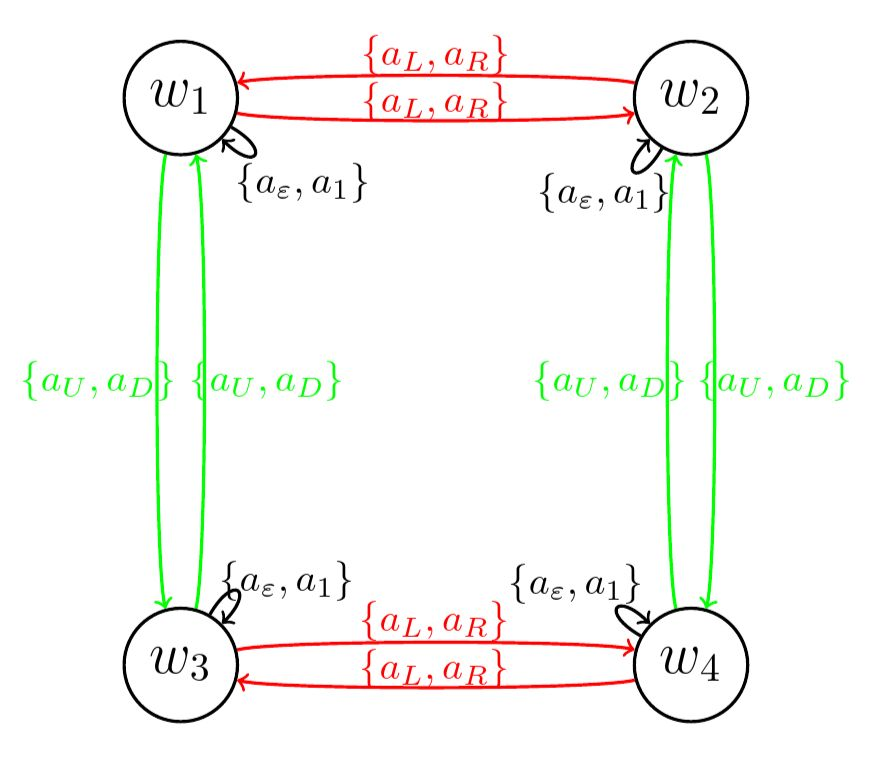
\includegraphics[width=0.75\linewidth]{2MathematicalFramework/Images/2x2_cyclical_equivalence_min_actions.jpeg}
    \caption{
    World diagram showing the equivalence classes under $\sim$ for the atomic actions and the empty action for the world-agent pair $\mathscr{W}_{\alpha}$-$\mathscr{A}$.
    \draftnote{purple}{PS}{
    Similar to \cref{fig:2x2_cyclical_labelling_with_min_actions}, put $\hat{A}^{*}$ diagram on the left with a $\pi_{\sim}$ labelled arrow pointing to the current figure on the right.
    }
    }
    \label{fig:2x2_cyclical_equivalence_min_actions}
\end{figure}

\draftnote{purple}{PS: Consider}{
\begin{enumerate}
    \item Diagram of map showing actions being sent to their equivalence classes under $\sim$: $D_{A}$ -($l$)-> $\hat{A}^{*}$ -($\pi_{A}$)-> $\hat{A}^{*}/\sim$.
\end{enumerate}
}

\whendraft{
\draftnote{red}{whendraft start}{}
%%%%%%%%%%%%%%%%%%%%%%%%%%%%%%%%%%%%%%%%
\section{
Equivalence on transformations
\draftnote{blue}{V0.5}{}
}

\draftnote{red}{Include}{
\begin{enumerate}
    \item (Put as footnote if there is no time) Equivalence relation $\sim$ for transformations and how it compares to equivalence relation $\sim$ for actions.
    \item Cannot apply the labelling map to $D/\sim$ to get $\hat{A}^{*}/\sim$.
    \item I think $\sim$ on $D$ matches the $\sim_{w}$'s.
\end{enumerate}
}

A natural analogue of our equivalence relation $\sim$ on actions is an equivalence relation, also denoted by $\sim$, on the transformations $D$ that equates two transforms is they both have the same sources and the same targets.
Formally, for $d, d' \in D$,
\begin{equation}
    d \sim d' \iff s(d) = s(d') \text{ and } t(d) = t(d')
\end{equation}
\draftnote{red}{whendraft end}{}
}

%%%%%%%%%%%%%%%%%%%%%%%%%%%%%%%%%%%%%%%%
\section{
Converting other equivalence relations
\texorpdfstring{to $\sim$}{}
\draftnote{blue}{V0.5}{}
}
\draftnote{red}{Include}{
\begin{enumerate}
    \item Formalism this section.
    \item Empirical example (using our algorithm).
    \item We can convert this into category theory quite easily I think (disjoint union).
\end{enumerate}
}

If we have another equivalence relation $\sim'$ on the actions in $\hat{A}^{*}$, we can transform the world $\mathscr{W}$ that $\sim'$ is being applied to and so harness what we have derived for the equivalence relation $\sim'$.

For example, let $\sim_{(t)}$ be defined as, for two actions $a, a' \in \hat{A}^{*}$,
\begin{align}
    & a \sim_{(t)} a' \iff a \ast w = a' \ast w \quad \text{ for all $w \in W$} \quad \text{and} \\
    & |a| \bmod t = |a'| \bmod t
\end{align}
We can transform any world $\mathscr{W}$, which we want to apply $\sim_{(t)}$ to, to a world $\mathscr{W}'$ when applying $\sim$ will produce the same algebraic structures as we would produce from applying $\sim_{(t=2)}$ to $\mathscr{W}$.
We do this by indexing each world state with the time\footnote{
Here we're taking time to be the number of atomic actions that have been performed from a given start time.
} $t \bmod 2$ that that world state can be visited at; then we split each world state with more than one index into that many new world states in $\mathscr{W}'$ connected with the relevant transformations with atomic action labels.

%%%%%%%%%%%%%%%%%%%%%%%%%%%%%%%%%%%%%%%%%%%%%%%%%%%%%%%%%
